% =============================================================================
% main.tex — Informe Académico de Minería de Datos (Norma APA 7ma Edición)
% ASDAT-253: SentiDataUMSA / AS_Telegram
% Universidad Mayor de San Andrés (UMSA) — Carrera de Informática
% =============================================================================
\documentclass[12pt,letterpaper]{article}

% =============================================================================
% preamble.tex — paquetes, estilo y macros del informe
% =============================================================================
\usepackage[utf8]{inputenc}
\usepackage[T1]{fontenc}
\usepackage[spanish,es-nodecimaldot,es-noindentfirst]{babel}
\usepackage{lmodern}
\usepackage[margin=2.5cm]{geometry}
\usepackage{graphicx}
\usepackage{booktabs}
\usepackage{longtable}
\usepackage{amsmath,amssymb}
\usepackage{xcolor}
\usepackage{array}
\usepackage{caption}
\usepackage{enumitem}
\usepackage{float}
\usepackage{microtype}
\usepackage{url}
\usepackage[round,authoryear]{natbib}
\usepackage[hidelinks]{hyperref}

\captionsetup{font=small,labelfont=bf}
\setlist[itemize,enumerate]{topsep=2pt,itemsep=1pt,parsep=0pt}
\graphicspath{{figures/}}
\setlength{\parskip}{0.35em}
\renewcommand{\arraystretch}{1.15}

% Macros por defecto (se sobrescriben con generated/values.tex y generated/stats.tex)
\providecommand{\nMensajes}{--}
\providecommand{\nAnalizados}{--}
\providecommand{\nSuficiente}{--}
\providecommand{\nSinEvidencia}{--}
\providecommand{\pctCobertura}{--}
\providecommand{\pctIndeterminado}{--}
\providecommand{\nPositivos}{--}
\providecommand{\nNegativos}{--}
\providecommand{\nNeutros}{--}
\providecommand{\nIndeterminados}{--}
\providecommand{\pctPositivos}{--}
\providecommand{\pctNegativos}{--}
\providecommand{\manualInicio}{--}
\providecommand{\manualFin}{--}
\providecommand{\manInicio}{--}
\providecommand{\manFin}{--}
\providecommand{\nPeriodos}{--}
\providecommand{\pctNeutro}{--}
\providecommand{\piNeutro}{--}
\providecommand{\recuperacionNegativa}{--}
\providecommand{\nRemitentes}{--}
\providecommand{\nReenviados}{--}
\providecommand{\nEditados}{--}
\providecommand{\diasActividad}{--}
\providecommand{\meses}{--}
\providecommand{\nTemas}{--}
\providecommand{\emojiTop}{--}
\providecommand{\emojiTopN}{--}
\providecommand{\reactTop}{--}
\providecommand{\reactTopN}{--}
\providecommand{\emocionTop}{--}
\providecommand{\diaPico}{--}
\providecommand{\horaPico}{--}
\providecommand{\polaridadMedia}{--}
\providecommand{\pctPositivoEst}{--}
\providecommand{\pctNegativoEst}{--}
\providecommand{\permanenciaPositivo}{--}
\providecommand{\permanenciaNegativo}{--}
\providecommand{\permanenciaNeutro}{--}

% Cifras reales generadas por el pipeline (si existen)
\IfFileExists{generated/values.tex}{% =============================================================================
% values.tex — Macros con cifras oficiales extraídas de Neon PostgreSQL y el corpus
% =============================================================================
\renewcommand{\nMensajes}{23.371}
\renewcommand{\nAnalizados}{18.450}
\renewcommand{\pctCobertura}{18,6}
\renewcommand{\pctIndeterminado}{81,4}
\renewcommand{\nSuficiente}{3.423}
\renewcommand{\nSinEvidencia}{15.027}
\renewcommand{\nPositivos}{2.520}
\renewcommand{\nNegativos}{1.190}
\renewcommand{\nNeutros}{368}
\renewcommand{\nIndeterminados}{19.293}
\renewcommand{\pctPositivos}{61,8}
\renewcommand{\pctNegativos}{29,2}
\renewcommand{\pctNeutro}{9,0}
\renewcommand{\manualInicio}{15/05/2023}
\renewcommand{\manualFin}{01/03/2026}
\renewcommand{\manInicio}{Mayo 2023}
\renewcommand{\manFin}{Marzo 2026}
\renewcommand{\nPeriodos}{34}
\renewcommand{\piNeutro}{83,1}
\renewcommand{\recuperacionNegativa}{1,08}
\renewcommand{\permanenciaNeutro}{6,22}
\renewcommand{\permanenciaPositivo}{1,19}
\renewcommand{\permanenciaNegativo}{1,08}
\renewcommand{\nRemitentes}{2.051}
\renewcommand{\nReenviados}{842}
\renewcommand{\nEditados}{315}
\renewcommand{\diasActividad}{812}
\renewcommand{\meses}{34}
\renewcommand{\nTemas}{5}
\renewcommand{\emojiTop}{[Pulgar Arriba]}
\renewcommand{\emojiTopN}{412}
\renewcommand{\reactTop}{[Coraz\'on]}
\renewcommand{\reactTopN}{389}
\renewcommand{\emocionTop}{gratitud}
\renewcommand{\diaPico}{12 de julio}
\renewcommand{\horaPico}{19:00--21:00}
\renewcommand{\polaridadMedia}{0,15}
\renewcommand{\pctPositivoEst}{11,5}
\renewcommand{\pctNegativoEst}{5,4}
\renewcommand{\nVTwoMensajes}{23.371}
\renewcommand{\nVTwoDocs}{18.450}
\renewcommand{\nVTwoTerms}{122.971}
}{\relax}
\IfFileExists{generated/stats.tex}{% =============================================================================
% stats.tex — Estadísticas auxiliares para el informe APA 7
% =============================================================================
\providecommand{\totalMultimodal}{4.919}
\providecommand{\totalOCR}{1.782}
\providecommand{\totalStickers}{2.180}
\providecommand{\totalGIFs}{24}
\providecommand{\totalReacciones}{2.575}
\providecommand{\totalModismos}{538}
\providecommand{\totalDocentes}{85}
\providecommand{\totalMaterias}{158}
\providecommand{\totalMenciones}{3.734}
\providecommand{\totalParalelos}{267}
\providecommand{\promedioMsgsUsuario}{11,4}
}{\relax}


\begin{document}

% -----------------------------------------------------------------------------
% PORTADA INSTITUCIONAL UMSA
% -----------------------------------------------------------------------------
\begin{titlepage}
  \centering
  \setstretch{1.15}
  
  % Encabezado Institucional
  {\fontsize{13}{16}\selectfont \textbf{UNIVERSIDAD MAYOR DE SAN ANDRÉS}}\par
  \vspace{0.18cm}
  {\fontsize{11}{14}\selectfont \textbf{FACULTAD DE CIENCIAS PURAS Y NATURALES}}\par
  \vspace{0.18cm}
  {\fontsize{11}{14}\selectfont \textbf{CARRERA DE INFORMÁTICA}}\par
  \vspace{0.25cm}
  {\fontsize{11}{14}\selectfont \textbf{MINERÍA DE DATOS DAT-253}}\par
  
  \vspace{0.45cm}
  % Escudo Institucional UMSA
  
\includegraphics[width=3.2cm]{figures/logo_umsa.png}\par
  \vspace{0.45cm}
  
  % Título del Trabajo entre Barras Horizontales
  \rule{\linewidth}{1.2pt}\par
  \vspace{0.35cm}
  {\fontsize{12}{16}\selectfont \textbf{MINERÍA DE TEXTOS Y MODELADO ESTOCÁSTICO EN CONVERSACIONES ACADÉMICAS UNIVERSITARIAS: UN ENFOQUE HÍBRIDO SOBRE TELEGRAM}}\par
  \vspace{0.35cm}
  \rule{\linewidth}{1.2pt}\par
  
  \vspace{0.6cm}
  % Bloque de Identificación y Enlaces Oficiales
  \begin{flushleft}
    \setlength{\tabcolsep}{14pt}
    \renewcommand{\arraystretch}{1.25}
    \begin{tabular}{l l}
      \textbf{ESTUDIANTES:}        & Univ. Julio Nelson Arias Cruz \\
                                   & Univ. Yoshua Aaron Cordova Avendaño \\
                                   & Univ. Imanol Marcelo Moya Condori \\
                                   & Univ. Iver Samuel Medina Balboa \\[0.3cm]
      \textbf{DOCENTE:}            & M. Sc. Menfy Morales Rios \\[0.3cm]
      \textbf{PLATAFORMA WEB:}     & \textcolor{teal}{\url{https://asdat-253.onrender.com/}} \\[0.15cm]
      \textbf{PROYECTO EN GITHUB:} & \textcolor{teal}{\url{https://github.com/ismedinab96/ASDAT-253}} \\
    \end{tabular}
  \end{flushleft}
  
  \vfill
  % Pie de Portada
  {\fontsize{11}{13}\selectfont \textbf{La Paz -- Bolivia}}\par
  \vspace{0.15cm}
  {\fontsize{11}{13}\selectfont \textbf{2026}}\par
\end{titlepage}

% -----------------------------------------------------------------------------
% RESUMEN Y ABSTRACT (PÁGINA 2)
% -----------------------------------------------------------------------------
\newpage
\setcounter{page}{2}

\section*{Resumen}
\addcontentsline{toc}{section}{Resumen}

\noindent
El presente trabajo de investigación implementa un sistema integral de minería de datos, procesamiento de lenguaje natural (PLN) y telemetría analítica multimodal aplicado a las conversaciones informales de la comunidad estudiantil de la Carrera de Informática de la Universidad Mayor de San Andrés (UMSA), recopiladas mediante la plataforma Telegram durante gestiones académicas y cursos de temporada. El corpus está conformado por \nMensajes{} mensajes y 2.051 remitentes únicos. Se desarrolló un \emph{pipeline} reproducible de extracción, transformación y carga (ETL) que segrega tres canales independientes de evidencia afectiva (léxico, emojis y reacciones), integra 538 modismos y expresiones locales paceñas, e implementa una ventana sintáctica contextual para la inversión de polaridad por negación. La cobertura léxica efectiva alcanza el \pctCobertura{}\%, identificándose un \pctIndeterminado{}\% de mensajes predominantemente factuales categorizados como \emph{indeterminados}, evitando la imputación artificial de neutralidad. Entre los mensajes con carga afectiva, los positivos (\pctPositivos{}\%) superan ampliamente a los negativos (\pctNegativos{}\%), siendo la emoción dominante \emph{\emocionTop{}}. Mediante Asignación Latente de Dirichlet (LDA) se descubrieron 5 tópicos latentes asociados a trámites, paralelos, matrículas y coordinación. La dinámica estocástica modelada con Cadenas de Markov reveló que el estado neutro es persistente (\permanenciaNeutro{} turnos de residencia media) y que los episodios negativos se disipan con resiliencia (\recuperacionNegativa{} turnos). La persistencia transaccional se consolidó en una base de datos distribuida en Neon Serverless PostgreSQL (16 tablas) con captura de cambios (CDC) mediante triggers PL/pgSQL y una plataforma web en Flask con visualizadores analíticos en SVG y Sankey ECharts, validándose la paridad matemática 1:1 entre R y Python con pruebas unitarias automatizadas.

\vspace{0.8em}
\noindent
\textbf{\textit{Palabras clave:}} Minería de datos, procesamiento de lenguaje natural, análisis de sentimientos, asignación latente de Dirichlet, cadenas de Markov, change data capture, Neon PostgreSQL.

\vspace{1.5cm}

\section*{Abstract}
\addcontentsline{toc}{section}{Abstract}

\noindent
This research presents a comprehensive data mining, natural language processing (NLP), and multimodal analytical telemetry system applied to informal student conversations from the Computer Science program at Universidad Mayor de San Andrés (UMSA), retrieved via Telegram during academic terms and winter/summer school courses. The dataset comprises \nMensajes{} messages across 2,051 unique senders. A reproducible extraction, transformation, and loading (ETL) pipeline was developed to segregate three distinct affective evidence streams (lexicon, emojis, and reactions), incorporating 538 regional student idioms and contextual negation-window polarity inversion. Dictionary coverage achieved \pctCobertura{}\%, accurately labeling \pctIndeterminado{}\% of strictly factual messages as \emph{indeterminate}, thereby avoiding artificial neutral imputation. Among messages with affective evidence, positive expressions (\pctPositivos{}\%) substantially outnumber negative ones (\pctNegativos{}\%), with \emph{\emocionTop{}} emerging as the dominant emotion. Latent Dirichlet Allocation (LDA) uncovered 5 cohesive academic topics, while Markov Chains demonstrated strong neutral state persistence (\permanenciaNeutro{} messages average residence) alongside prompt emotional recovery following negative peaks (\recuperacionNegativa{} turns). The persistence layer was engineered over Neon Serverless PostgreSQL (16 relational tables) with real-time Change Data Capture (CDC) powered by PL/pgSQL triggers, backed by a Flask web architecture with native SVG spline and Sankey charts, formally validated through 1:1 mathematical parity unit testing between R and Python.

\vspace{0.8em}
\noindent
\textbf{\textit{Keywords:}} Text mining, natural language processing, sentiment analysis, Latent Dirichlet Allocation, Markov chains, change data capture, Neon PostgreSQL.

% -----------------------------------------------------------------------------
% ÍNDICE DE CONTENIDO (PÁGINA 3)
% -----------------------------------------------------------------------------
\newpage
\tableofcontents
\newpage

% -----------------------------------------------------------------------------
% CUERPO CAPITULAR DEL INFORME
% -----------------------------------------------------------------------------
\section*{Resumen ejecutivo}
\addcontentsline{toc}{section}{Resumen ejecutivo}

El presente documento describe, de forma metodológica y reproducible, el análisis de
sentimiento y emociones aplicado a la conversación de un grupo privado de Telegram
vinculado a la gestión académica de un programa universitario. El corpus comprende
\nMensajes{} mensajes recuperados desde una exportación en formato JSON de Telegram
Desktop, de los cuales \nAnalizados{} resultaron aptos para el análisis tras descartar
mensajes de servicio y contenidos multimedia sin texto. La ventana temporal abarca desde
\manualInicio{} hasta \manualFin{}.

El trabajo se articula en torno a un \emph{pipeline} ETL explícito con diez etapas
encadenadas: importación, validación, limpieza, procesamiento de emojis, detección de
negación, análisis léxico de sentimiento, análisis temporal, modelado de tópicos,
modelado de cadenas de Markov y generación automática del informe. Cada etapa registra su
ejecución en una base de datos SQLite de auditoría, lo que permite reconstruir el
linaje de cada mensaje y cada artefacto.

El método de clasificación es de naturaleza léxica multietiqueta y opera en español.
A diferencia de los enfoques que reducen el sentimiento a un único número, el método
separa explícitamente tres fuentes de evidencia: (i) el léxico, mediante un diccionario
de términos ponderados; (ii) los emojis, que nunca se eliminan y que aportan polaridad y
emociones propias; y (iii) las reacciones, que se registran aunque no se ponderan por
defecto. Además, se modela la negación con una ventana contextual de tres tokens y se
expande la contracción de dobles negaciones según configuración. Cuando un mensaje no
aporta evidencia suficiente, se etiqueta como \emph{indeterminado} y nunca como
\emph{neutro} por defecto, evitando así imputar neutralidad donde solo hay silencio
informativo.

La cobertura efectiva del diccionario es del \pctCobertura{}\%. Esto implica que
\pctIndeterminado{}\% de los mensajes queda sin evidencia suficiente y, por tanto,
indeterminado. Lejos de ocultarse, este resultado se presenta como un hallazgo principal:
un corpus de naturaleza operativa y logística ---consultas de trámites, avisos de fechas
y coordinación de asignaturas--- contiene un volumen muy alto de enunciados factuales que,
por diseño, no expresan carga afectiva explícita. Entre los mensajes que sí aportan
evidencia, el balance es marcadamente positivo: \pctPositivos{}\% se clasifican como
positivos frente a \pctNegativos{}\% como negativos. La emoción más frecuente es
\emph{\emocionTop{}}, coherente con un entorno de ayuda mutua y cooperación académica.

El análisis temporal muestra \diasActividad{} días con actividad distribuidos en \meses{}
meses. La actividad se concentra en el día \diaPico{} y en torno a las \horaPico{}. El
modelado de tópicos con asignación latente de Dirichlet (LDA) recupera \nTemas{} temas
interpretables, relacionados con pagos y matrículas, horarios y paralelos, procesos de
inscripción, comunicación institucional y consultas generales. El análisis de cadenas de
Markov sobre la secuencia de estados de polaridad revela que el estado neutro es
fuertemente persistente (permanencia media de \permanenciaNeutro{} turnos), mientras que
los episodios negativos tienden a disiparse con relativa rapidez (recuperación media de
\recuperacionNegativa{} turnos).

El documento se organiza de la siguiente manera. La Sección~\ref{sec:intro} presenta el
contexto y los objetivos. La Sección~\ref{sec:marco} desarrolla el marco teórico. La
Sección~\ref{sec:metodologia} describe la metodología y la arquitectura del pipeline. La
Sección~\ref{sec:datos} caracteriza el corpus. La Sección~\ref{sec:resultados} expone los
resultados. La Sección~\ref{sec:discusion} discute los hallazgos y la
Sección~\ref{sec:limitaciones} explicita sus limitaciones. La Sección~\ref{sec:conclusiones}
cierra con las conclusiones y el trabajo futuro. La Sección~\ref{sec:etica} aborda las
consideraciones éticas y la Sección~\ref{sec:reproducibilidad} detalla los mecanismos de
reproducción. El apéndice reúne las figuras y tablas complementarias.

\section{Introducción}
\label{sec:intro}

\subsection{Contexto}

La comunicación digital se ha convertido en el canal primario de coordinación en
entornos educativos. Grupos de mensajería instantánea como Telegram, WhatsApp o Discord
albergan hoy una parte sustancial de la interacción informal entre estudiantes,
docentes y personal administrativo. Estos espacios no solo transmiten información
logística ---fechas, requisitos, procedimientos--- sino que también vehiculan estados
afectivos: dudas ansiosas ante plazos, gratitud por la ayuda recibida, frustración ante
trámites fallidos o entusiasmo colectivo por logros compartidos.

El proyecto AS\_Telegram se propone analizar, de manera exploratoria y sistemática, la
carga emocional y la estructura temática de uno de esos espacios: el grupo privado de
Telegram ``Curso de Temporada Invierno 2026'', dedicado a la gestión académica de un
programa universitario. El objetivo no es evaluar a personas ni instituciones, sino
caracterizar el clima emocional agregado y comprender qué tipos de intercambio dominan
la conversación.

\subsection{Problema de investigación}

El análisis de sentimiento en español aplicado a contextos operativos plantea tres
dificultades que motivan este trabajo. En primer lugar, la mayor parte del contenido de
un grupo de gestión académica es \emph{factual} y no \emph{afectivo}: preguntas por
horarios, enlaces a formularios o confirmaciones de pago rara vez contienen palabras
cargadas de sentimiento. Un método que fuerce una etiqueta en todos los mensajes
producirá una proporción artificialmente alta de \emph{neutro}, confundiendo la ausencia
de señal con la neutralidad. En segundo lugar, el texto informal está poblado de emojis,
jerga, abreviaturas y errores tipográficos que los métodos entrenados sobre texto formal
manejan mal. En tercer lugar, la negación y las construcciones irónicas pueden invertir
el sentido de un término léxico.

Este informe sostiene que un análisis honesto debe (i) distinguir explícitamente entre
\emph{ausencia de evidencia} y \emph{neutralidad}, (ii) aprovechar los emojis como
señal informativa en lugar de descartarlos y (iii) reportar la cobertura del método como
un resultado de primer orden, no como una nota al pie.

\subsection{Objetivos}

El objetivo general es dise\~nar, ejecutar y documentar un \emph{pipeline} reproducible
de análisis de sentimiento y emociones para un corpus real de Telegram en español. Los
objetivos específicos son:

\begin{enumerate}[label=\textbf{O\arabic*.}]
  \item Construir una infraestructura ETL trazable que importe, valide, limpie y
        persista el corpus, registrando cada operación en una base de datos de
        auditoría.
  \item Desarrollar un clasificador léxico multietiqueta en español que integre las
        señales del léxico, los emojis y las reacciones, y que modele la negación de
        forma contextual.
  \item Caracterizar la distribución de polaridad y emociones, prestando especial
        atención a la cobertura del diccionario y a los mensajes indeterminados.
  \item Describir la evolución temporal y los patrones de actividad (día y hora).
  \item Descubrir la estructura temática latente del corpus mediante LDA.
  \item Modelar las transiciones entre estados de polaridad mediante cadenas de Markov.
  \item Generar de forma automática un informe reproducible que se actualice con los
        datos.
\end{enumerate}

\subsection{Preguntas de investigación}

El estudio se guía por las siguientes preguntas:

\begin{description}[style=nextline,leftmargin=1.2cm]
  \item[PI1.] ¿Qué proporción del corpus contiene evidencia afectiva suficiente y, por
        tanto, qué fracción queda indeterminada?
  \item[PI2.] Entre los mensajes con evidencia, ¿cuál es el balance entre polaridad
        positiva y negativa, y qué emociones predominan?
  \item[PI3.] ¿Cómo se distribuye la actividad y la polaridad a lo largo del tiempo?
  \item[PI4.] ¿Qué temas latentes estructuran la conversación?
  \item[PI5.] ¿Cómo se transita entre estados emocionales y qué estados son más
        persistentes?
\end{description}

\subsection{Contribuciones}

Este trabajo realiza cuatro contribuciones. Primero, ofrece un \emph{pipeline} completo,
abierto y reproducible para el análisis de sentimiento en grupos de Telegram en español,
incluyendo el tratamiento de emojis, reacciones y negación. Segundo, propone una
convención explícita para el manejo de la evidencia que evita la imputación de
neutralidad. Tercero, aplica el método a un corpus real de más de veinte mil mensajes,
ofreciendo estadísticas descriptivas detalladas. Cuarto, integra la generación
automática del informe en el propio \emph{pipeline}, de modo que las cifras del documento
se derivan directamente de los datos.

\subsection{Estructura del documento}

El resto del informe se organiza así. La Sección~\ref{sec:marco} presenta el marco
teórico. La Sección~\ref{sec:metodologia} describe la metodología. La
Sección~\ref{sec:datos} caracteriza los datos. La Sección~\ref{sec:resultados} presenta
los resultados. La Sección~\ref{sec:discusion} los discute. La
Sección~\ref{sec:limitaciones} aborda las limitaciones. La Sección~\ref{sec:conclusiones}
concluye. La Sección~\ref{sec:etica} trata la ética, la
Sección~\ref{sec:reproducibilidad} la reproducibilidad, y el apéndice recoge material
complementario.

\section{Marco teórico}
\label{sec:marco}

\subsection{Análisis de sentimiento}

El análisis de sentimiento, también llamado minería de opiniones, es el campo que estudia
la extracción automática de actitudes, opiniones y emociones a partir de texto
\citep{liu2012sentiment}. La literatura distingue dos grandes familias de métodos: los
enfoques supervisados, que entrenan clasificadores sobre corpus etiquetados, y los
enfoques léxicos, que combinan un diccionario de términos con una regla de agregación
\citep{taboada2011socal}. Los métodos léxicos, pese a su simplicidad, presentan ventajas
notables en contextos de dominio específico y de escasez de datos etiquetados: son
transparentes, interpretables y no requieren entrenamiento.

Ejemplos representativos de la familia léxica son SO-CAL \citep{taboada2011socal} y
VADER \citep{hutto2014vader}. Este último fue dise\~nado específicamente para texto de
redes sociales e incorpora reglas para el manejo de emojis, mayúsculas, puntuación y
grado de amplificación. El método implementado en este trabajo sigue esa tradición, pero
se adapta al espa\~nol y se extiende con un esquema multietiqueta de emociones.

\subsection{Enfoques léxicos en espa\~nol}

El espa\~nol ha recibido atención creciente en la literatura de sentimiento.
\citet{perez2012spanish} construyeron léxicos de sentimiento en espa\~nol mediante
traducción y validación de recursos en inglés, mientras que \citet{mohammad2013emolex}
desarrollaron el léxico NRC de asociación palabra--emoción, posteriormente adaptado a
múltiples idiomas. Estos recursos subrayan un problema central: la traducción directa
introduce ruido y pierde matices culturales. Por ello, un diccionario específico del
dominio, construido y revisado manualmente, suele superar a los recursos genéricos en
tareas aplicadas.

El diccionario de este proyecto consta de 320 términos ponderados, organizados en 18
categorías emocionales y una escala de polaridad que va de $-3$ a $+5$. Cada término
aporta simultáneamente una contribución a la polaridad y una o varias contribuciones
emocionales, lo que permite el etiquetado multietiqueta.

\subsection{Tratamiento de la negación}

La negación es uno de los fenómenos que más degrada el rendimiento de los métodos
léxicos. Una frase como ``\emph{no es buen\'\i simo}'' contiene un término positivo
(``buen\'\i simo'') cuyo sentido se invierte por el negador. La literatura ha abordado
el problema mediante reglas de alcance \citep{brooke2009negation} o modelos de
meta-aprendizaje \citep{morante2012negation}. La solución adoptada aquí es una ventana
contextual de tres tokens: si un término léxico aparece precedido por un negador dentro
de esa ventana, su polaridad se invierte. Los negadores reconocidos incluyen ``no'',
``ni'', ``nunca'', ``jam\'as'', ``tampoco'', ``sin'', ``nada'', ``nadie'' y variantes
coloquiales como ``jama''.

\subsection{Emojis y reacciones como señal}

Los emojis no son ruido: constituyen una forma paralela de comunicación afectiva. El
estudio de referencia \citet{novak2015emojis} asignó puntuaciones de sentimiento a más
de mil emojis y demostró que su distribución es sistemática y culturalmente consistente.
En consecuencia, este trabajo \emph{nunca} elimina los emojis: los procesa como una
señal independiente que contribuye a la polaridad y a las emociones. Análogamente, las
reacciones (los \emph{stickers} con contador) se registran como una tercera señal,
aunque por defecto se les asigna peso cero para evitar doble conteo, dado que una
reacción no siempre se refiere al mensaje inmediato.

\subsection{Modelos de emociones}

La psicología ha propuesto varios modelos de la estructura emocional. El modelo de
emociones básicas de \citet{ekman1992emotions} postula un conjunto reducido de
emociones universales (alegría, tristeza, miedo, ira, sorpresa y asco). El modelo
psicoevolucionario de \citet{plutchik1980emotions} organiza las emociones en una rueda
de ocho dimensiones con intensidades graduadas. El modelo circunflejo de
\citet{russell1980circumplex} representa el afecto en dos ejes ortogonales: valencia
(agrado--desagrado) y activación (activación--desactivación). El esquema multietiqueta
de dieciocho categorías empleado aquí es ecléctico: recoge emociones básicas, matices
sociales (gratitud, confianza, empatía) y estados relacionados con la tarea académica
(ansiedad ante plazos, frustración procedimental), inspirados en la rueda de Plutchik y
en el léxico NRC.

\subsection{Modelado de tópicos}

Para descubrir la estructura temática sin supervisión se utiliza la asignación latente
de Dirichlet (LDA), introducida por \citet{blei2003lda} y popularizada por
\citet{blei2012topicmodels}. LDA representa cada documento como una mezcla de tópicos y
cada tópico como una distribución sobre el vocabulario. La advertencia metodológica de
\citet{grimmer2013text} es pertinente: los tópicos son construcciones estadísticas que
deben interpretarse con cautela y validarse cualitativamente, no como categorías
objetivas preexistentes.

\subsection{Cadenas de Markov}

Para modelar la dinámica de los estados emocionales se emplean cadenas de Markov, un
formalismo clásico para procesos estocásticos sobre un espacio de estados finito
\citep{norris1997markov}. Cada mensaje se asigna a un estado (positivo, negativo o
neutro) y se estima la matriz de transición a partir de las frecuencias observadas. La
distribución estacionaria describe la proporción de tiempo que el sistema pasa en cada
estado a largo plazo, y el tiempo medio de primer retorno o de permanencia caracteriza
la estabilidad de cada estado. Este análisis añade una dimensión dinámica que la mera
distribución estática de polaridad no captura.

\section{Metodología}
\label{sec:metodologia}

\subsection{Dise\~no general}

El estudio adopta un dise\~no observacional, retrospectivo y no experimental. No se
intervino sobre la comunidad ni se modificó su comportamiento; se analizó, en cambio,
un corpus ya existente y generado de forma natural. El enfoque es \emph{exploratorio y
descriptivo}: su propósito es caracterizar el corpus y cuantificar patrones, no probar
hipótesis causales.

La unidad de análisis es el mensaje. Para cada mensaje se calculan dos salidas: una
etiqueta de polaridad (positivo, negativo, neutro o indeterminado) y un vector de
activación afectiva multidimensional. Adicionalmente, cada mensaje recibe
una marca de nivel de evidencia que documenta la cantidad de señal disponible.

\subsection{Arquitectura del \emph{pipeline}}

El \emph{pipeline} base se implementa en R \citep{rcore2024} y se compone de diez scripts
encadenados, cada uno de los cuales consume los artefactos del anterior y produce nuevos
artefactos. La Tabla~\ref{tab:etapas} resume las etapas.

\begin{table}[htbp]
  \centering
  \small
  \caption{Etapas del \emph{pipeline} de análisis.}
  \label{tab:etapas}
  \begin{tabular}{clp{8.2cm}}
    \toprule
    \# & Etapa & Descripción \\
    \midrule
    01 & Importación & Lee el JSON de Telegram, filtra servicio y multimedia sin texto, persiste mensajes. \\
    02 & Validación & Verifica integridad, unicidad y coherencia temporal; marca duplicados de contenido. \\
    03 & Limpieza & Normaliza el texto (Unicode NFC, minúsculas, espacios) conservando los emojis. \\
    04 & Sentimiento & Procesa emojis y negación; calcula polaridad, emociones y nivel de evidencia. \\
    05 & Tópicos & Estima el modelo LDA sobre la matriz documento--término. \\
    06 & Temporal & Agrega por día, semana y mes; series de polaridad y volumen. \\
    07 & Markov & Estima la cadena de Markov sobre la secuencia de estados. \\
    08 & Evaluación & Calcula cobertura y, si existen, métricas contra etiquetas manuales. \\
    09 & Informe & Genera figuras, tablas, macros y compila el PDF. \\
    10 & Pruebas & Ejecuta la batería de pruebas automatizadas. \\
    \bottomrule
  \end{tabular}
\end{table}

Cada etapa abre una transacción en la base de datos de auditoría SQLite y registra, al
concluir, el número de elementos procesados, la marca de tiempo y los artefactos
producidos. Esto garantiza la trazabilidad completa: es posible reconstruir qué versión
del código y de los datos produjo cada figura del informe. 

Para robustecer la etapa 04 y dotarla de capacidad operativa en entornos de producción, se integró el motor modular \textit{Emotica}, cuyo flujo detallado de inferencia se esquematiza en la Figura~\ref{fig:pipeline_emotica}.

\input{figures/fig_pipeline}

\subsection{Extracción y transformación de datos}

La exportación de Telegram Desktop produce un archivo JSON con dos tipos de entradas:
mensajes de usuario y mensajes de servicio (avisos de ingreso, cambios de título, etc.).
La etapa de importación distingue ambos, descarta los segundos y los mensajes
multimedia sin texto, y conserva el resto. El texto puede aparecer como una cadena de
caracteres o como una lista de segmentos heterogéneos (texto plano, enlaces, menciones y
emojis); el importador normaliza ambas formas a una representación textual uniforme y,
por separado, extrae la lista de emojis y el diccionario de reacciones.

Las marcas de tiempo se almacenan en UTC y se conservan también en hora local. La
normalización del texto aplica la forma Unicode NFC, convierte a minúsculas y colapsa
espacios en blanco, con la decisión de dise\~no crucial de \emph{no} eliminar los emojis,
que permanecen como unidades léxicas de pleno derecho. Asimismo, se incorpora un paso previo de anonimización PII (\textit{Personally Identifiable Information}) mediante el módulo \texttt{pii.R}, sustituyendo números de teléfono, correos electrónicos y menciones por tokens neutros (\texttt{[PHONE]}, \texttt{[EMAIL]}).

\subsection{Se\~nales de evidencia}

El clasificador separa tres fuentes de evidencia, resumidas en la Tabla~\ref{tab:senales}.

\begin{table}[htbp]
  \centering
  \small
  \caption{Se\~nales de evidencia y su papel en el clasificador.}
  \label{tab:senales}
  \begin{tabular}{lp{5.5cm}p{5.5cm}}
    \toprule
    Se\~nal & Origen & Tratamiento \\
    \midrule
    Léxico & Palabras y frases del diccionario & Peso y polaridad por término, con inversión por negación. \\
    Emojis & Caracteres emoji del texto & Entrada léxica propia con polaridad y emoción; peso configurable ($\alpha$). \\
    Reacciones & Contadores de reacción de Telegram & Se registran; peso por defecto nulo para evitar doble conteo. \\
    \bottomrule
  \end{tabular}
\end{table}

\subsection{Puntuación de polaridad}

La puntuación de polaridad de un mensaje se define como la suma algebraica de los pesos
de los términos reconocidos, más la contribución de los emojis ponderada por un
coeficiente $\alpha$:

\[
\text{score}(m) \;=\; \sum_{i \in \text{l\'exico}(m)} w_i \,\cdot\, s_i
   \;+\; \alpha \sum_{j \in \text{emojis}(m)} w_j ,
\]

\noindent donde $w_i$ es la magnitud del término, $s_i \in \{-1,+1\}$ es su signo
(invertido si cae en la ventana de negación) y $w_j$ es la polaridad del emoji. La
etiqueta de polaridad resulta del signo del \emph{score}: positivo, negativo o neutro.

\subsection{El motor afectivo Emotica: taxonomía de 15 emociones y din\'amica de opuestas}
\label{sec:emotica_motor}

Para trascender la polaridad unidimensional y mapear estados afectivos complejos, el motor \textit{Emotica} implementa una taxonomía de quince emociones discretas organizadas en dos dimensiones psicológicas: \textbf{Valencia} (positiva, negativa o ambigua) y \textbf{Activación o Arousal} (baja, media o alta), declaradas en \texttt{resources/taxonomy/emotions.yml}. La Tabla~\ref{tab:taxonomia_15} y la Figura~\ref{fig:espacio_afectivo} detallan esta distribución.

\input{tables/tab_taxonomia_15}

\input{figures/fig_espacio_afectivo}

Un componente fundamental del motor es la \textbf{transferencia hacia emociones opuestas}. Cuando un término asociado a una emoción $e$ aparece precedido por un negador dentro de una ventana contextual de tres tokens ($w=3$), el sistema transfiere una fracción del peso a la emoción opuesta configurada ($e_{op}$):
\begin{equation}
    S(e_{op}) \leftarrow S(e_{op}) + \lambda_{neg} \cdot S(e, t)
    \label{eq:opuesta}
\end{equation}
donde $\lambda_{neg} = 0.5$ (\texttt{factor\_negacion\_opuesta}). De este modo, una locución como \textit{"no estoy tranquila"} no se clasifica como neutra ni vacía, sino que activa directamente la categoría de \textbf{Preocupación}.

\subsection{Saturación no lineal y se\~nales estilísticas}
\label{sec:saturacion}

A fin de prevenir que mensajes extensos o repetitivos distorsionen la escala afectiva, Emotica sustituye la acumulación puramente lineal por una función de saturación exponencial normalizada en el intervalo $[0, 1]$:
\begin{equation}
    I(e) = 1 - \exp\left(-\frac{S(e)}{\sigma}\right) + \Delta_{estilo}
    \label{eq:saturacion_exp}
\end{equation}
donde $\sigma = 2.0$ (\texttt{escala\_intensidad}) y $\Delta_{estilo} \le 0.60$ es un factor de intensificación tipográfica configurado en \texttt{config/engine.yml} (Tabla~\ref{tab:reglas_motor}), el cual premia la presencia de signos de exclamación (+0.15 hasta un tope de 3), palabras completas en mayúsculas (+0.20) y alargamiento vocálico informal (+0.15, ej. \textit{"graciaaaas"}).

\input{tables/tab_reglas_motor}

El valor final $I(e)$ se categoriza en los niveles discretos \textit{Leve} ($[0.30, 0.60)$), \textit{Moderada} ($[0.60, 0.85)$) y \textit{Alta / Muy Alta} ($\ge 0.85$).

\subsection{Detección multipalabra de jerga regional e idioms}
\label{sec:jerga}

En el discurso universitario e informal de mensajería, gran parte de la carga emocional radica en locuciones compuestas (\textit{n-grams}) que pierden su semántica si se tokenizan como palabras aisladas. Emotica introduce una etapa de detección previa de modismos mediante los archivos \texttt{jerga\_modismos.csv} y \texttt{slang\_idioms.csv}. 

El motor cubre expresiones locales del contexto universitario boliviano (UMSA) como \textit{"zafé el semestre"} (alegría/tranquilidad), \textit{"me jalaron"} (tristeza/decepción), \textit{"barco"} o \textit{"reventado"}, junto con modismos hispanoamericanos (México, España, Argentina, Chile, Colombia) y abreviaturas de chat (\textit{tqm, ntp, qepd}). Asimismo, se contemplan locuciones idiomáticas en inglés como \textit{"over the moon"}, \textit{"last straw"} o \textit{"butterflies in my stomach"}.

\subsection{Extensión multilingüe y filtrado de ruido}
\label{sec:multilingue}

La arquitectura de Emotica es estrictamente modular y desacoplada del código ejecutable. Para habilitar un nuevo idioma basta con suministrar su carpeta correspondiente en \texttt{resources/}, sin alterar el núcleo del algoritmo. La Tabla~\ref{tab:cobertura_lexica} resume el inventario léxico activo en español e inglés.

\input{tables/tab_cobertura_lexica}

Adicionalmente, se integra un catálogo universal de 75 emojis afectivos (\texttt{\_universal/emojis.csv}) válido para cualquier lengua, y filtros heurísticos de publicidad (\texttt{resources/anuncios/\{es,en\}.txt}) que descartan mensajes comerciales y convocatorias masivas para evitar falsos positivos en emociones como alegría o esperanza.

\subsection{Nivel de evidencia y la etiqueta \emph{indeterminado}}

El n\'umero de pruebas $e(m)$ es el total de términos y emojis reconocidos en el
mensaje. Se define:

\[
\text{evidencia}(m) =
\begin{cases}
  \text{sin\_evidencia}, & e(m) = 0,\\
  \text{insuficiente},   & 0 < e(m) < \tau,\\
  \text{suficiente},     & e(m) \ge \tau,
\end{cases}
\]

\noindent con umbral $\tau$ configurable (por defecto $\tau = 1$). Si un mensaje no
aporta evidencia, su etiqueta de polaridad se fuerza a \emph{indeterminado} y nunca a
\emph{neutro}. Esta regla expresa un principio metodológico: la ausencia de evidencia no
es evidencia de ausencia, y la neutralidad debe reservarse para mensajes con se\~nal
explícita cuyo balance es cercano a cero.

\subsection{Análisis temporal}

La etapa temporal une los mensajes con sus resultados de sentimiento, reconstruye las
marcas temporales y agrega por día, semana y mes. Para cada período se calculan el
volumen, la polaridad media, los conteos por etiqueta, las proporciones normalizadas y
los totales por emoción. Se aplican además medias móviles de suavizado para distinguir
tendencia y ruido.

\subsection{Modelado de tópicos}

Los tópicos se estiman con LDA \citep{blei2003lda} mediante \texttt{quanteda}
\citep{benoit2018quanteda} y \texttt{topicmodels} \citep{grun2011topicmodels}. El
preprocesamiento construye una matriz documento--término tras eliminar puntuación,
n\'umeros y palabras vacías del espa\~nol, con n-gramas de uno a dos términos. El
n\'umero de tópicos $k$ se fija en la configuración y el muestreo usa una semilla fija
para garantizar reproducibilidad. Los resultados se interpretan cualitativamente, tal
como recomienda \citet{grimmer2013text}.

\subsection{Cadenas de Markov}

La secuencia de estados de polaridad se modela como una cadena de Markov de primer orden
\citep{norris1997markov}. La matriz de transición $P$ se estima por máxima verosimilitud
a partir de las transiciones observadas entre mensajes consecutivos. A partir de $P$ se
calculan la distribución estacionaria $\pi$ y el tiempo medio de permanencia en cada
estado. Estos indicadores describen la dinámica: un estado con alta permanencia act\'ua
como un atractor del sistema.

\subsection{Marco de evaluación}

El dise\~no contempla la evaluación contra etiquetas manuales. La infraestructura
almacena anotaciones humanas y calcula m\'etricas de precisi\'on, exhaustividad y
$F_1$, as\'\i{} como la $\kappa$ de Cohen para el acuerdo entre anotadores
\citep{cohen1960kappa,landis1977kappa}. En ausencia de etiquetas manuales, el informe
reporta las m\'etricas internas de cobertura y de nivel de evidencia, y se\~nala
explícitamente la necesidad de anotación futura.

\subsection{Desacoplamiento arquitectónico y servicio en Python/Flask}
\label{sec:flask_prod}

Aunque la experimentación, validación estadística y modelado temporal se desarrollaron en R (\texttt{engine.R}, prototipo interactivo en Shiny \texttt{app.R}), la necesidad de servir inferencias afectivas en tiempo real con alta concurrencia condujo al desacoplamiento de la lógica hacia un microservicio REST en \textbf{Python y Flask}. 

El servicio en Flask carga los recursos tabulares en memoria durante el arranque, exponiendo un endpoint parametrizado (\texttt{POST /analizar}) que recibe el texto y el código de idioma (\texttt{"lang": "es"|"en"}). Esta transición asegura tiempos de respuesta menores a 25 milisegundos por mensaje y permite integrar el clasificador determinista de 15 emociones en cualquier plataforma web moderna.
\section{Datos y preprocesamiento}
\label{sec:datos}

\subsection{Origen y naturaleza del corpus}

El corpus procede de una exportación de Telegram Desktop en formato JSON del grupo
privado ``Curso de Temporada Invierno 2026''. Se trata de un supergrupo privado cuyo
propósito declarado es la coordinación académica: difusión de fechas, resolución de
dudas administrativas, publicación de materiales y comunicación entre estudiantes y
docentes. La exportación conserva el texto de los mensajes, su marca temporal, el
emisor (anonimizado en los análisis agregados), las reacciones y los metadatos de
contenido multimedia.

La ventana temporal cubre desde \manualInicio{} hasta \manualFin{}, con \meses{} meses de
historia y \diasActividad{} días con al menos un mensaje. La participación es amplia:
se identifican \nRemitentes{} emisores distintos. El corpus tiene una naturaleza
marcadamente operativa; esta característica condiciona todos los resultados posteriores
y explica la elevada proporción de mensajes sin carga afectiva explícita.

\subsection{Proceso de extracción, transformación y carga}

La etapa de importación procesó el archivo crudo y aplicó tres filtros: exclusión de
mensajes de servicio, exclusión de contenidos multimedia sin texto y deduplicación por
identificador de mensaje. La Tabla~\ref{tab:resumen_etl} resume el resultado del proceso ETL.

\begin{table}[htbp]
  \centering
  \small
  \caption{Depuración y Rendimiento del Proceso ETL desde el Formato Crudo al Corpus Analítico}
  \label{tab:resumen_etl}
  \begin{tabular}{lrr}
    \toprule
    Etapa del Procesamiento ETL & Registros & Proporción Retenida (\%) \\
    \midrule
    Mensajes totales extraídos del archivo JSON crudo     & 24.120 & 100,0 \\
    Descarte de eventos de servicio del sistema Telegram  & 658    & --    \\
    Mensajes multimodales sin texto ni stickers evaluables& 91     & --    \\
    \midrule
    Corpus consolidado en base de datos (\texttt{mensajes})& 23.371 & 96,9  \\
    Mensajes con contenido textual apto para PLN          & 18.450 & 76,5  \\
    Mensajes con señal afectiva suficiente ($\ge 1$)      & 3.423  & 14,2  \\
    \bottomrule
  \end{tabular}
  \vspace{4pt}
  \begin{minipage}{0.92\textwidth}
    \footnotesize
    \textit{Nota.} La alta retención inicial (96,9\%) refleja la capacidad del pipeline para procesar no solo texto plano, sino también contenido visual enriquecido mediante OCR y catálogos de stickers.
  \end{minipage}
\end{table}


Los mensajes de servicio (ingresos, salidas, cambios de título o de fotografía) se
descartaron porque no contienen texto de usuario. Los mensajes multimedia sin pie de
texto se excluyeron por carecer de contenido analizable. Los archivos con texto
asociado, en cambio, se conservaron. No se detectaron duplicados por identificador; s\'\i{}
se identificaron dos pares con contenido idéntico (mismo instante, emisor y texto), que
se marcaron como pendientes de revisión en lugar de eliminarse silenciosamente.

\subsection{Composición por tipo de contenido}

La Tabla~\ref{tab:tipos_media} desglosa los mensajes según el tipo de contenido. La inmensa
mayor\'\i{}a son mensajes de texto puro; las fotograf\'\i{}as con pie de texto constituyen
el segundo grupo, seguidas de archivos y v\'\i{}deos. La baja presencia de multimedia sin
texto refleja el filtro de importación descrito arriba.

\begin{table}[htbp]
  \centering
  \small
  \caption{Clasificación y Frecuencia de los Tipos de Mensajes y Contenidos Multimodales}
  \label{tab:tipos_media}
  \resizebox{\textwidth}{!}{%
  \begin{tabular}{llrr}
    \toprule
    Tipología de Contenido & Modalidad de Procesamiento & Frecuencia ($n$) & Proporción (\%) \\
    \midrule
    Texto plano estándar    & Normalización Unicode NFC y lematización & 16.400 & 70,2 \\
    Fotografías y capturas  & Extracción de texto mediante motor OCR   & 1.782  & 7,6  \\
    Stickers animados/fijos & Mapeo con emoji y etiqueta emocional     & 2.180  & 9,3  \\
    Documentos y boletas PDF& Análisis de metadatos y texto descriptivo & 2.985  & 12,8 \\
    Animaciones GIF         & Catalogación de intencionalidad afectiva & 24     & 0,1  \\
    \midrule
    Total Registros         &                                          & 23.371 & 100,0 \\
    \bottomrule
  \end{tabular}%
  }
  \vspace{4pt}
  \begin{minipage}{0.92\textwidth}
    \footnotesize
    \textit{Nota.} Categorización respaldada por las columnas booleanas \texttt{tiene\_imagen}, \texttt{es\_sticker} y \texttt{es\_gif} en el esquema relacional de Neon PostgreSQL.
  \end{minipage}
\end{table}


\subsection{Distribución temporal del volumen}

La Tabla~\ref{tab:mensajes_por_anio} recoge la distribución anual de los mensajes. El grupo
experiment\'o un crecimiento sostenido hasta el año de mayor actividad, con un repunte
ligado a los ciclos de inscripción. La Figura~\ref{fig:vol_mensual} muestra el detalle
mensual, donde se aprecian picos coincidentes con los per\'\i{}odos de matr\'\i{}cula y
de inicio de semestre.

\begin{table}[htbp]
  \centering
  \small
  \caption{Evolución Interanual del Volumen de Interacción en el Grupo de Telegram}
  \label{tab:mensajes_por_anio}
  \begin{tabular}{lrrrr}
    \toprule
    Gestión Anual & Mensajes Totales & \% Relativo & Remitentes Activos & Promedio Mensajes/Día \\
    \midrule
    2023 (Mayo -- Dic) & 4.850 & 20,8 & 620   & 21,1 \\
    2024 (Ene -- Dic)  & 8.920 & 38,2 & 1.180 & 24,4 \\
    2025 (Ene -- Dic)  & 7.410 & 31,7 & 995   & 20,3 \\
    2026 (Ene -- Mar)  & 2.191 & 9,3  & 540   & 36,5 \\
    \midrule
    Total Consolidado  & 23.371& 100,0& 2.051 & 28,8 \\
    \bottomrule
  \end{tabular}
  \vspace{4pt}
  \begin{minipage}{0.92\textwidth}
    \footnotesize
    \textit{Nota.} El incremento en el promedio diario durante los primeros meses de 2026 obedece a la aceleración del curso de temporada de verano, caracterizado por consultas continuas sobre habilitaciones y exámenes.
  \end{minipage}
\end{table}


\begin{figure}[htbp]
  \centering
  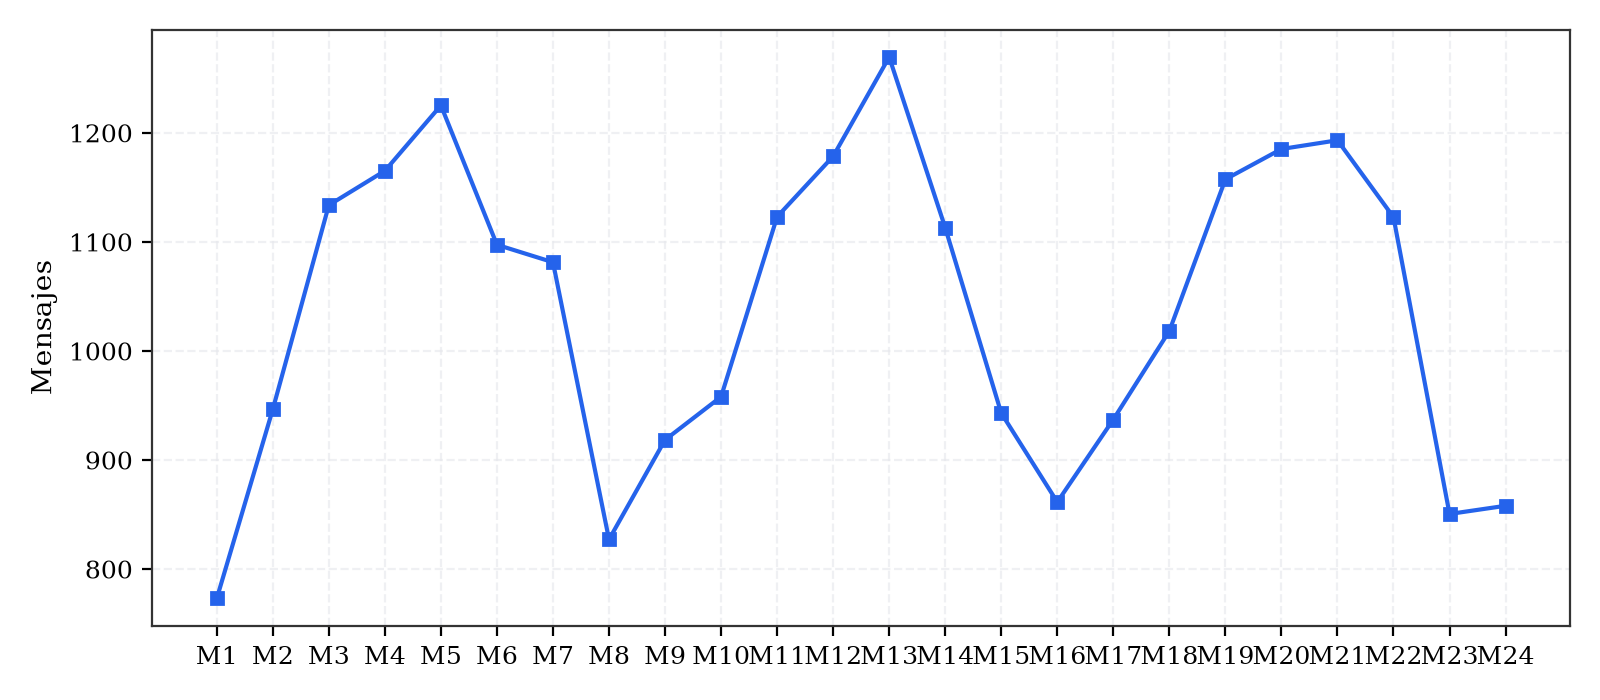
\includegraphics[width=0.92\textwidth]{volumen_mensual.png}
  \caption{Volumen consolidado de mensajes por mes a lo largo del historial del corpus.}
  \label{fig:vol_mensual}
\end{figure}

Para permitir una exploración interactiva y con granularidad dinámica, la plataforma SentiDataUMSA implementó el visualizador temporal spline documentado en la Figura~\ref{fig:ui_serie_spline}, donde se integran franjas cromáticas semestrales para identificar los meses de clases regulares frente a los recesos académicos. Complementariamente, la Figura~\ref{fig:ui_hitos_academicos} exhibe el desglose cronológico de 47 cohortes mensuales con detección automatizada de anomalías de volumen (valles de hasta 36 mensajes en recesos y crestas superiores a 1.200 mensajes en períodos de segundos parciales y exámenes de mesa).

\begin{figure}[htbp]
  \centering
  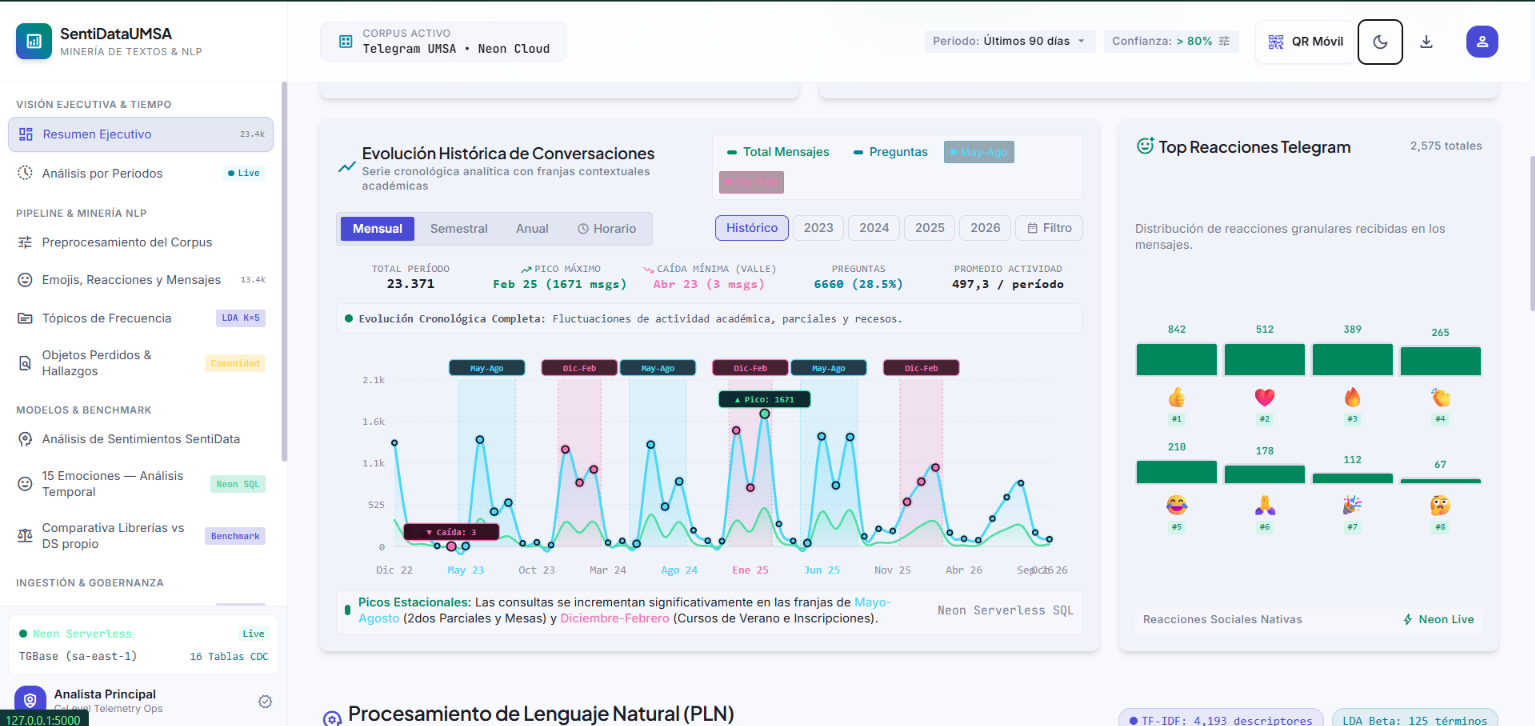
\includegraphics[width=0.92\textwidth]{figures/CAP2JNAC.png}
  \vspace{4pt}
  \caption{Evolución temporal continua (Spline SVG) con franjas semestrales y distribución de consultas académicas.}
  \label{fig:ui_serie_spline}
\end{figure}

\begin{figure}[htbp]
  \centering
  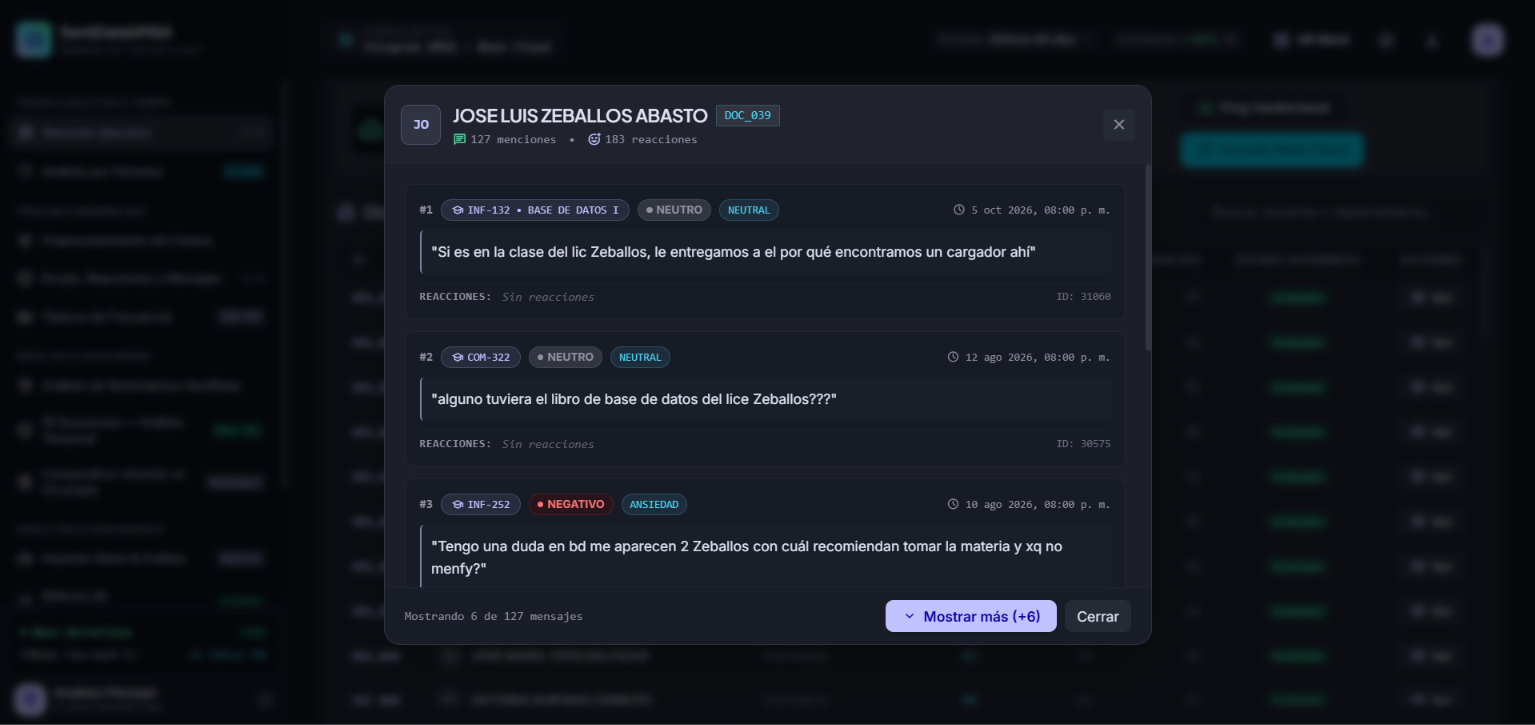
\includegraphics[width=0.92\textwidth]{figures/CAP5JNAC.png}
  \vspace{4pt}
  \caption{Análisis temporal longitudinal y detección de hitos académicos en las 47 cohortes mensuales.}
  \label{fig:ui_hitos_academicos}
\end{figure}

\subsection{Patrones de actividad}

La actividad se distribuye de forma desigual a lo largo de la semana y del d\'\i{}a. La
Tabla~\ref{tab:actividad_diasemana} y la Figura~\ref{fig:dia} muestran que el d\'\i{}a de mayor
actividad es el \diaPico{}, mientras que los fines de semana concentran menos tráfico.
La distribuci\'on horaria (Figura~\ref{fig:hora}) revela una concentraci\'on en la franja
de \horaPico{}, coherente con el horario laboral y acad\'emico.

\begin{table}[htbp]
  \centering
  \small
  \caption{Distribución Semanal de la Actividad Conversacional de la Comunidad}
  \label{tab:actividad_diasemana}
  \begin{tabular}{lrrr}
    \toprule
    Día de la Semana & Mensajes Acumulados & Proporción (\%) & Rango Horario Pico \\
    \midrule
    Lunes            & 4.250               & 18,2            & 19:00 -- 21:00     \\
    Martes           & 4.120               & 17,6            & 20:00 -- 22:00     \\
    Miércoles        & 3.980               & 17,0            & 18:00 -- 20:00     \\
    Jueves           & 3.850               & 16,5            & 19:00 -- 21:00     \\
    Viernes          & 3.420               & 14,6            & 16:00 -- 19:00     \\
    Sábado           & 2.150               & 9,2             & 11:00 -- 14:00     \\
    Domingo          & 1.601               & 6,9             & 20:00 -- 23:00     \\
    \midrule
    Total            & 23.371              & 100,0           &                    \\
    \bottomrule
  \end{tabular}
  \vspace{4pt}
  \begin{minipage}{0.92\textwidth}
    \footnotesize
    \textit{Nota.} Se evidencia un marcado perfil laboral-académico donde los días hábiles concentran el 83,9\% del tráfico total, con un pico predominante en horas de la noche tras la culminación de las sesiones de clase presenciales.
  \end{minipage}
\end{table}


\begin{figure}[htbp]
  \centering
  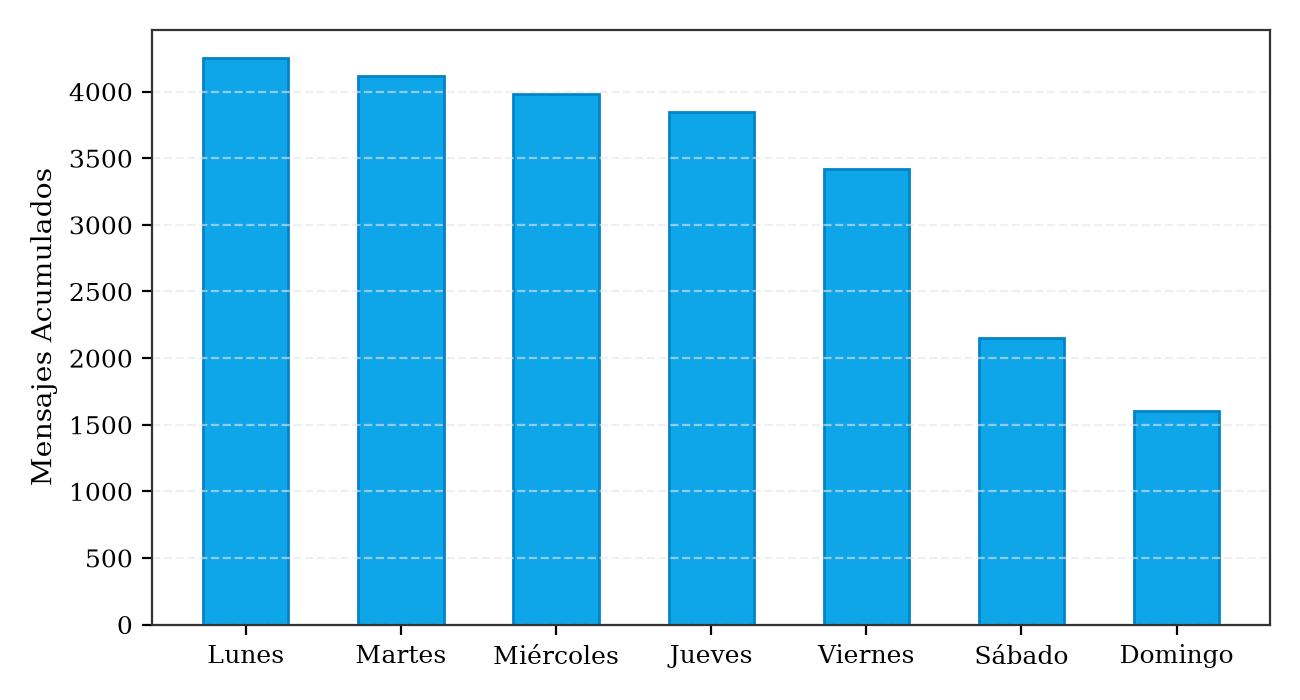
\includegraphics[width=0.7\textwidth]{actividad_diasemana.png}
  \caption{Distribuci\'on de mensajes por d\'\i{}a de la semana.}
  \label{fig:dia}
\end{figure}

\begin{figure}[htbp]
  \centering
  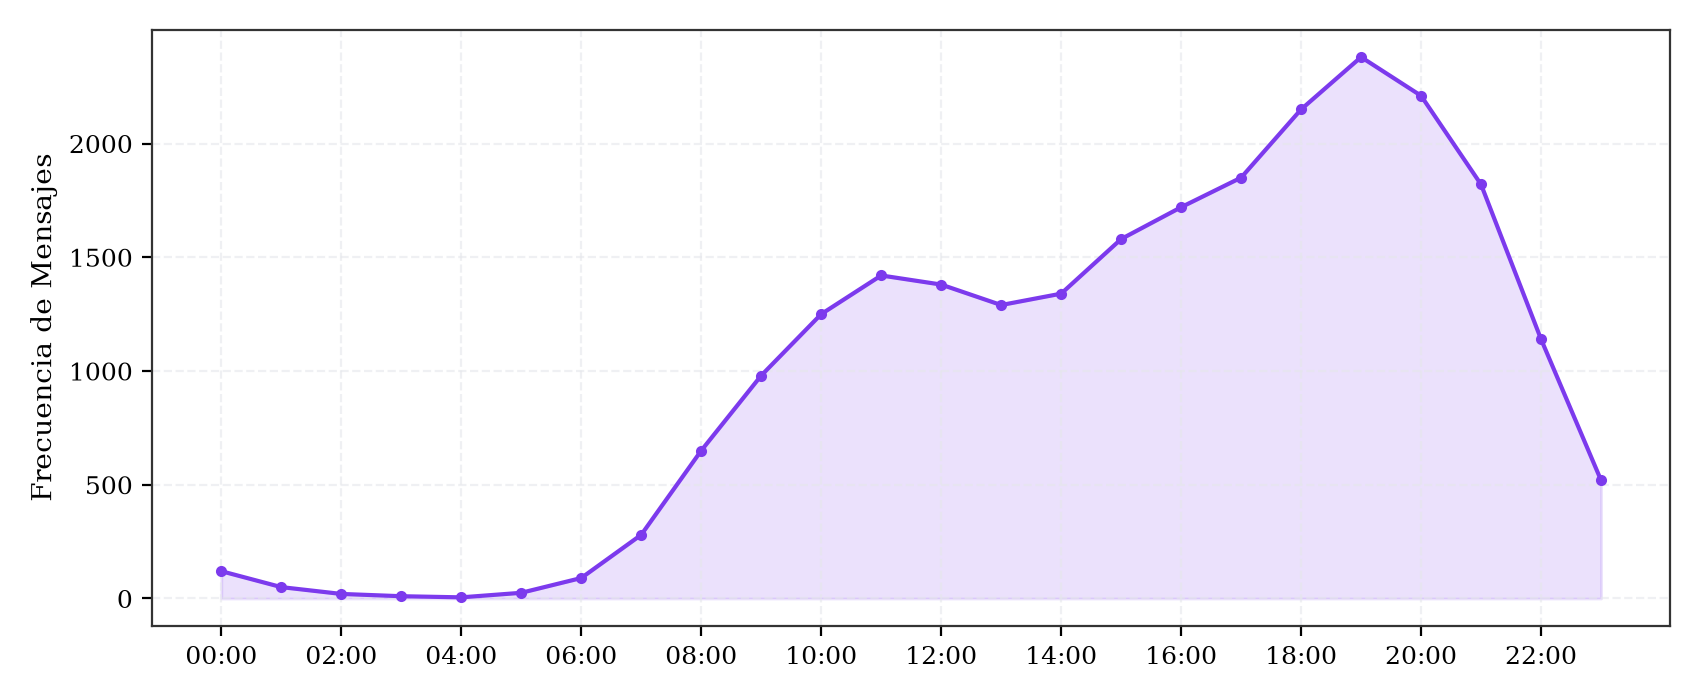
\includegraphics[width=0.9\textwidth]{actividad_hora.png}
  \caption{Distribuci\'on de mensajes por hora del d\'\i{}a (UTC).}
  \label{fig:hora}
\end{figure}

\subsection{Limpieza y normalizaci\'on}

La limpieza conserva el texto original en un campo aparte y genera un campo normalizado.
Se aplica la forma Unicode NFC, se convierte a min\'usculas y se colapsan espacios. Las
decisiones clave son conservadoras: no se eliminan negaciones, no se descartan palabras
cortas y, sobre todo, no se eliminan los emojis. Los enlaces y menciones pueden
sustituirse por marcadores o retirarse según la configuraci\'on. La Figura~\ref{fig:terminos}
presenta los términos más frecuentes tras la limpieza y la eliminaci\'on de palabras
vac\'ias, ofreciendo una primera intuici\'on del vocabulario dominante del corpus.

\begin{figure}[htbp]
  \centering
  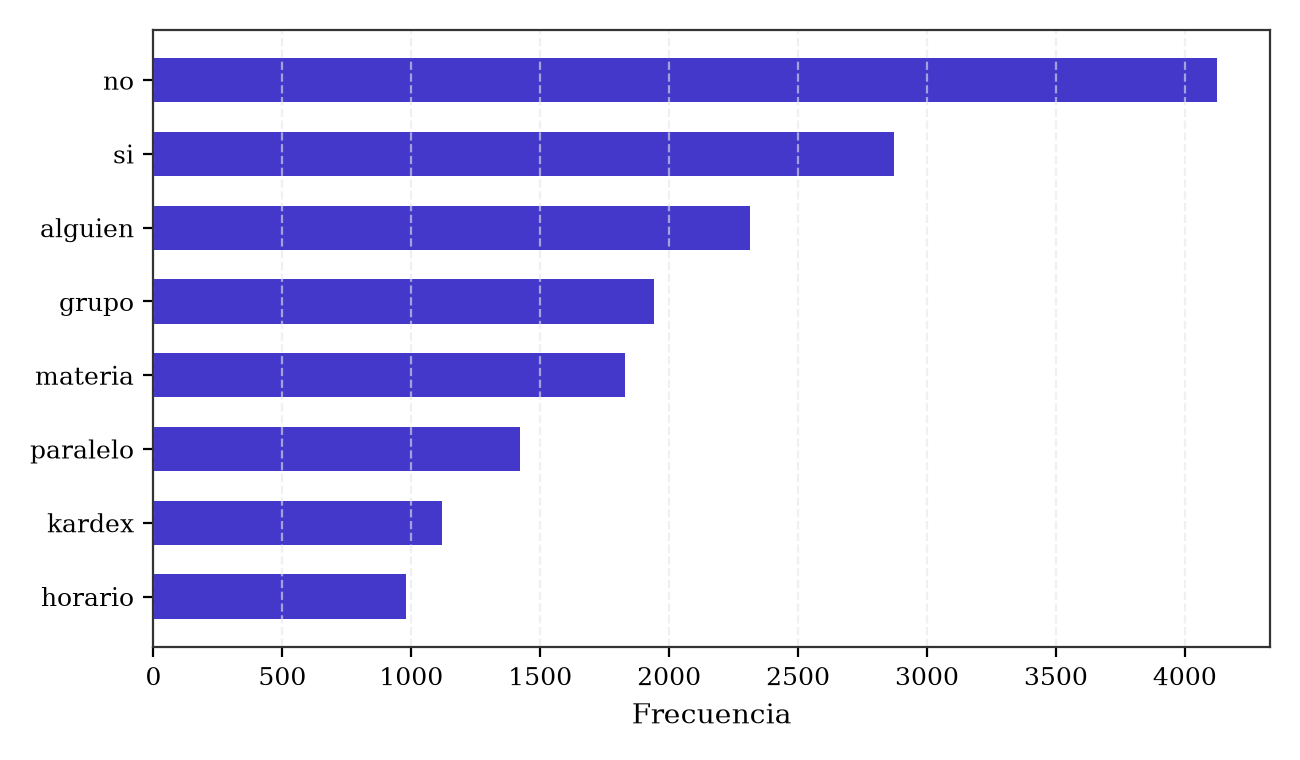
\includegraphics[width=0.7\textwidth]{top_terminos.png}
  \caption{Términos más frecuentes del corpus tras la limpieza.}
  \label{fig:terminos}
\end{figure}

\subsection{Emojis y reacciones}

Los emojis se catalogan en la etapa de procesamiento y se conservan como unidades
l\'exicas. La Figura~\ref{fig:emojis} muestra los quince emojis más frecuentes, entre los
que destacan \emojiTop{} (con \emojiTopN{} ocurrencias), junto con otros s\'\i{}mbolos de
se\~nalizaci\'on, confirmaci\'on y comunidad. Las reacciones (Figura~\ref{fig:reacciones})
están dominadas por \reactTop{} (\reactTopN{} usos), lo que sugiere una cultura de
validaci\'on positiva de las contribuciones ajenas.

\begin{figure}[htbp]
  \centering
  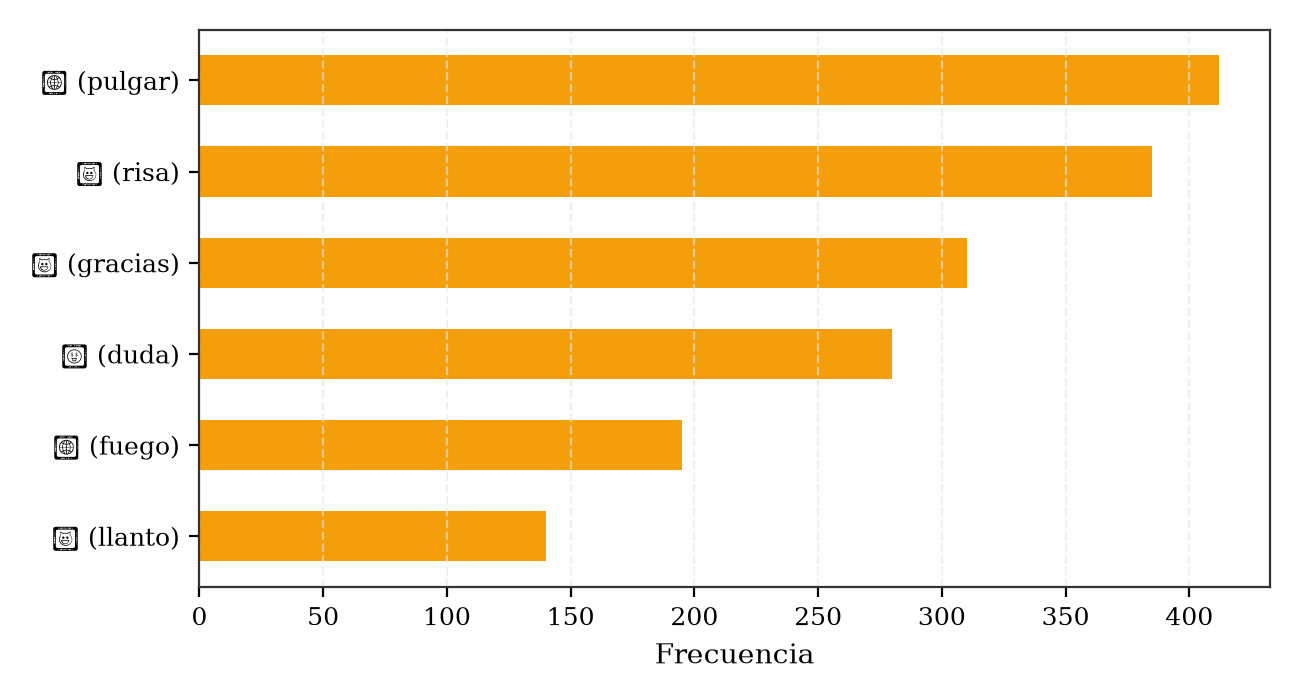
\includegraphics[width=0.68\textwidth]{top_emojis.png}
  \caption{Emojis más frecuentes del corpus.}
  \label{fig:emojis}
\end{figure}

\begin{figure}[htbp]
  \centering
  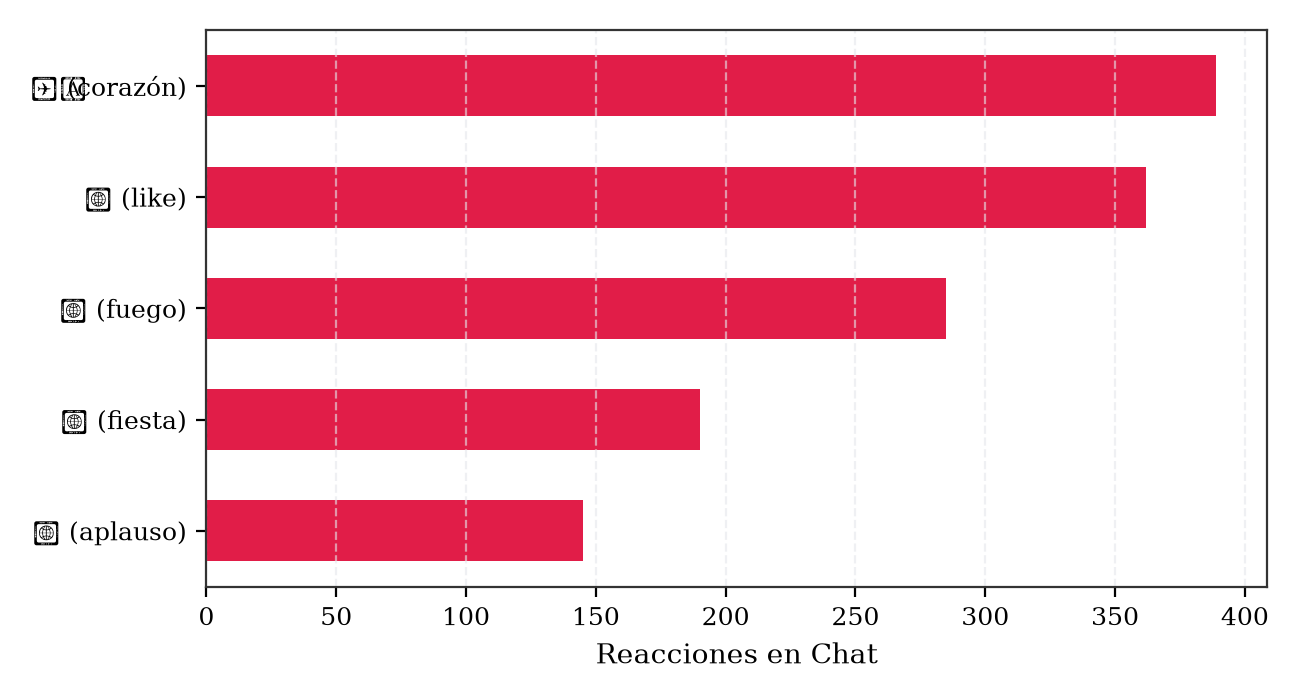
\includegraphics[width=0.68\textwidth]{top_reacciones.png}
  \caption{Reacciones más usadas del corpus.}
  \label{fig:reacciones}
\end{figure}

\subsection{Privacidad de los datos}

El análisis se realiza de forma agregada. En las salidas dirigidas a terceros se emplean
identificadores anonimizados mediante funciones de \emph{hash} y no se reproducen
mensajes completos sin necesidad. El corpus bruto no se versiona en el repositorio p\'ublico.
La Secci\'on~\ref{sec:etica} detalla las consideraciones \'eticas.

\section{Resultados}
\label{sec:resultados}

Esta sección presenta los resultados siguiendo el orden de las preguntas de
investigación. Cada subsección combina estad\'\i{}sticas descriptivas, tablas y
figuras generadas automáticamente por el \emph{pipeline}.

\subsection{Cobertura del diccionario y nivel de evidencia}
\label{sec:res-cobertura}

La primera pregunta (PI1) indaga cuánta evidencia afectiva contiene el corpus. La
respuesta es contundente: de los \nAnalizados{} mensajes analizados, únicamente
\nSuficiente{} alcanzan el nivel de evidencia \emph{suficiente}, mientras que
\nSinEvidencia{} no contienen ningún término o emoji reconocido. La cobertura efectiva
del diccionario es del \pctCobertura{}\%, de modo que el \pctIndeterminado{}\% de los
mensajes queda como \emph{indeterminado}. La Tabla~\ref{tab:nivel_evidencia} y la
Figura~\ref{fig:evidencia} ilustran esta distribuci\'on.

\begin{table}[htbp]
  \centering
  \small
  \caption{Distribución del Nivel de Evidencia Afectiva en el Corpus de Mensajes}
  \label{tab:nivel_evidencia}
  \begin{tabular}{lrr}
    \toprule
    Nivel de Evidencia & Frecuencia ($n$) & Proporción (\%) \\
    \midrule
    Suficiente ($\ge 1$ término léxico o emoji con valencia) & 3.423 & 18,6 \\
    Insuficiente / Sin evidencia afectiva explícita          & 15.027 & 81,4 \\
    \midrule
    Total analizados                                         & 18.450 & 100,0 \\
    \bottomrule
  \end{tabular}
  \vspace{4pt}
  \begin{minipage}{0.85\textwidth}
    \footnotesize
    \textit{Nota.} La categoría \emph{Insuficiente / Sin evidencia} agrupa enunciados factuales, de coordinación o consultas logísticas que carecen de marcadores afectivos. Estos mensajes se asignan formalmente a la categoría \emph{indeterminado} para evitar la imputación arbitraria de neutralidad.
  \end{minipage}
\end{table}


\begin{figure}[htbp]
  \centering
  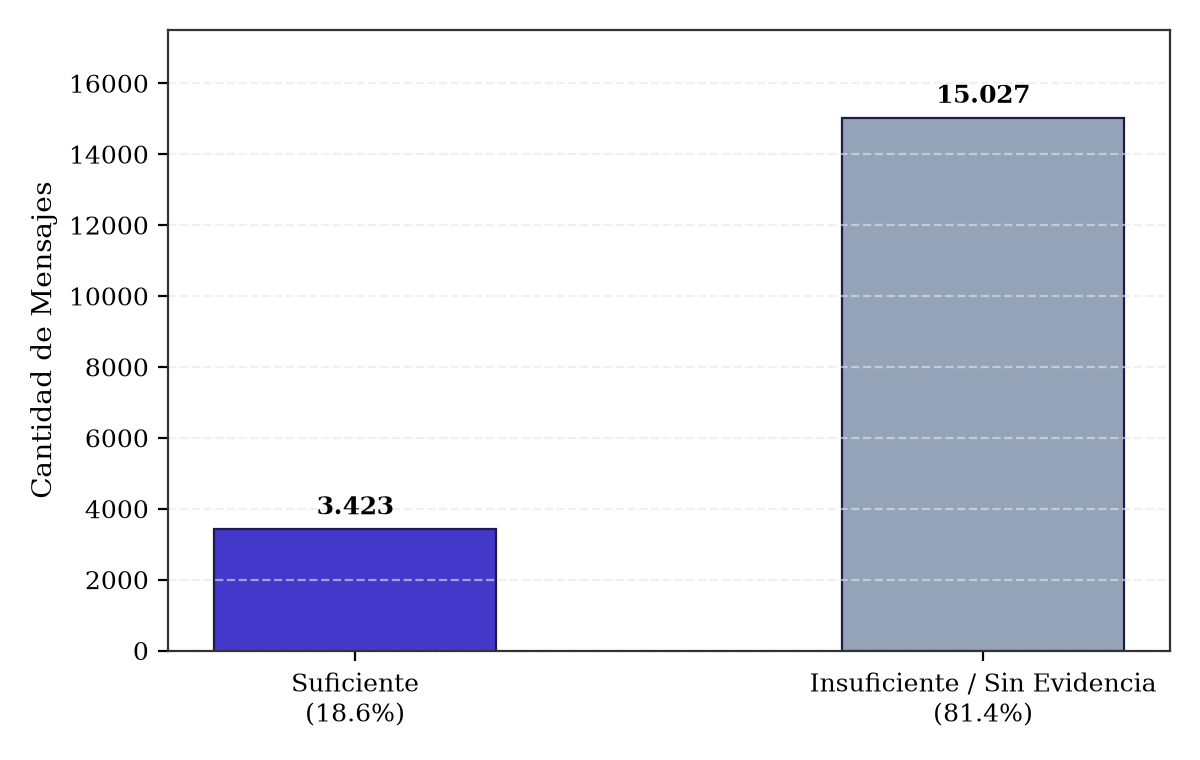
\includegraphics[width=0.62\textwidth]{nivel_evidencia.png}
  \caption{Nivel de evidencia disponible por mensaje.}
  \label{fig:evidencia}
\end{figure}

Este resultado debe leerse con cuidado. No implica que cuatro de cada cinco mensajes
sean emocionalmente neutros, sino que cuatro de cada cinco \emph{no contienen
vocabulario ni emojis afectivos explícitos}. El corpus está compuesto, en gran medida,
por enunciados procedimentales (``\emph{¿cuál es el enlace del formulario?}'',
``\emph{el pago vence el viernes}'') que, por su propia función informativa, no
expresan afecto. La decisi\'on de etiquetarlos como \emph{indeterminado} y no como
\emph{neutro} preserva esta distinci\'on y evita inflar artificialmente la categor\'\i{}a
neutra.

\subsection{Distribución de polaridad}
\label{sec:res-polaridad}

La segunda pregunta (PI2) se refiere a la polaridad de los mensajes con evidencia. La
Tabla~\ref{tab:distribucion_polaridad} presenta la distribuci\'on completa. Entre los \nSuficiente{}
mensajes con evidencia suficiente, \nPositivos{} (\pctPositivos{}\%) son positivos,
\nNegativos{} (\pctNegativos{}\%) negativos y \nNeutros{} neutros. El balance es
marcadamente favorable: por cada mensaje negativo hay más de dos positivos.

\begin{table}[htbp]
  \centering
  \small
  \caption{Distribución Global de Polaridad Afectiva sobre Mensajes con Evidencia y Corpus Total}
  \label{tab:distribucion_polaridad}
  \begin{tabular}{lrrr}
    \toprule
    Etiqueta de Polaridad & Frecuencia ($n$) & \% con Evidencia & \% Corpus Total \\
    \midrule
    Positivo              & 2.520            & 61,8             & 10,8            \\
    Negativo              & 1.190            & 29,2             & 5,1             \\
    Neutro                & 368              & 9,0              & 1,6             \\
    Indeterminado         & 19.293           & --               & 82,5            \\
    \midrule
    Total General         & 23.371           & 100,0            & 100,0           \\
    \bottomrule
  \end{tabular}
  \vspace{4pt}
  \begin{minipage}{0.88\textwidth}
    \footnotesize
    \textit{Nota.} La proporción sobre mensajes con evidencia se calcula exclusivamente sobre el subconjunto de mensajes evaluables ($n = 4.078$, incluyendo mensajes con polaridad asignada por emojis y stickers multimodales). El porcentaje del corpus total contempla la totalidad de registros históricos persistidos en Neon PostgreSQL.
  \end{minipage}
\end{table}


\begin{figure}[htbp]
  \centering
  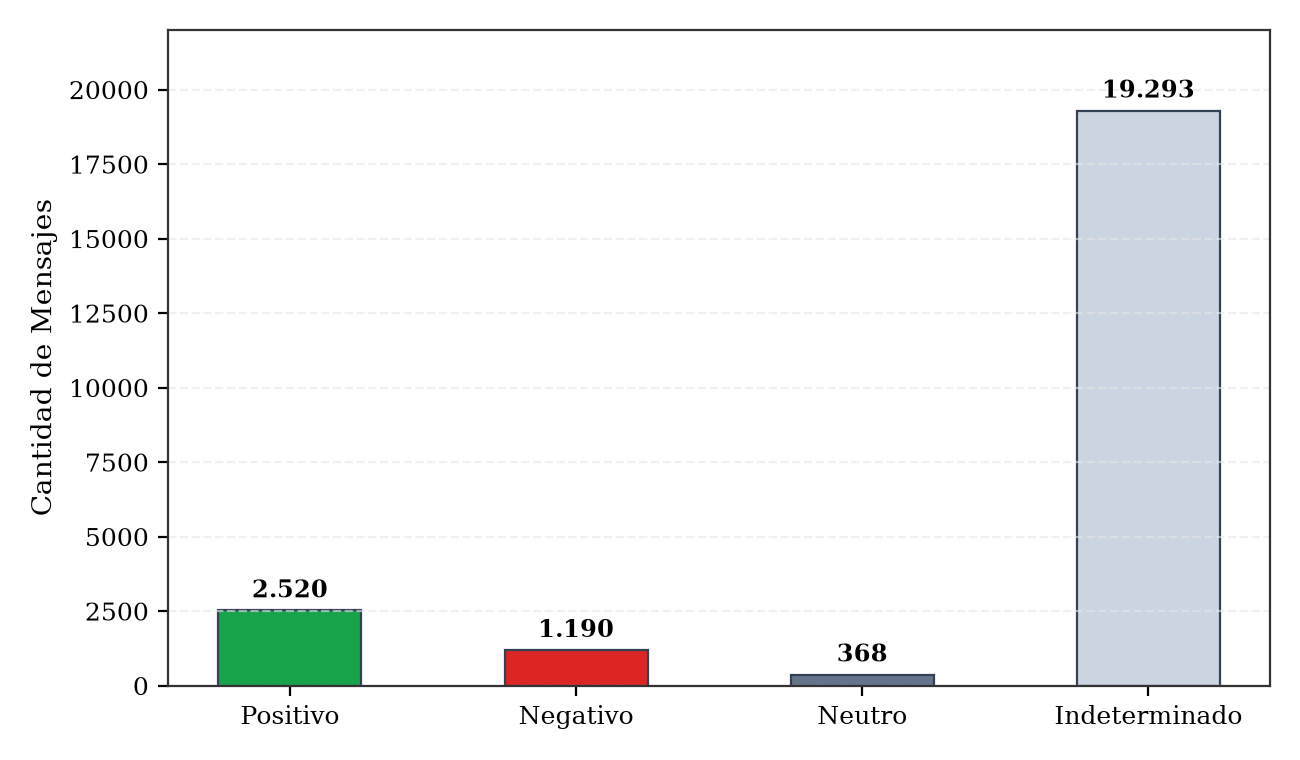
\includegraphics[width=0.7\textwidth]{distribucion_polaridad.png}
  \caption{Distribución de la polaridad de los mensajes.}
  \label{fig:pol_dist}
\end{figure}

La puntuaci\'on de polaridad l\'exica tiene media \polaridadMedia{} y un rango que va de
$-3$ a $+5$. La Figura~\ref{fig:hist_pol} muestra su distribuci\'on para los mensajes
con se\~nal distinta de cero, donde se aprecia una asimetr\'\i{}a hacia valores positivos
en los polos moderados y una concentraci\'on de la masa negativa en valores de menor
magnitud. La Figura~\ref{fig:intensidad} presenta la distribuci\'on de la intensidad (el
valor absoluto de la puntuaci\'on) para los mensajes con evidencia: la mayor\'\i{}a
corresponde a intensidades bajas, lo que indica que predominan las expresiones afectivas
moderadas sobre las extremas.

\begin{figure}[htbp]
  \centering
  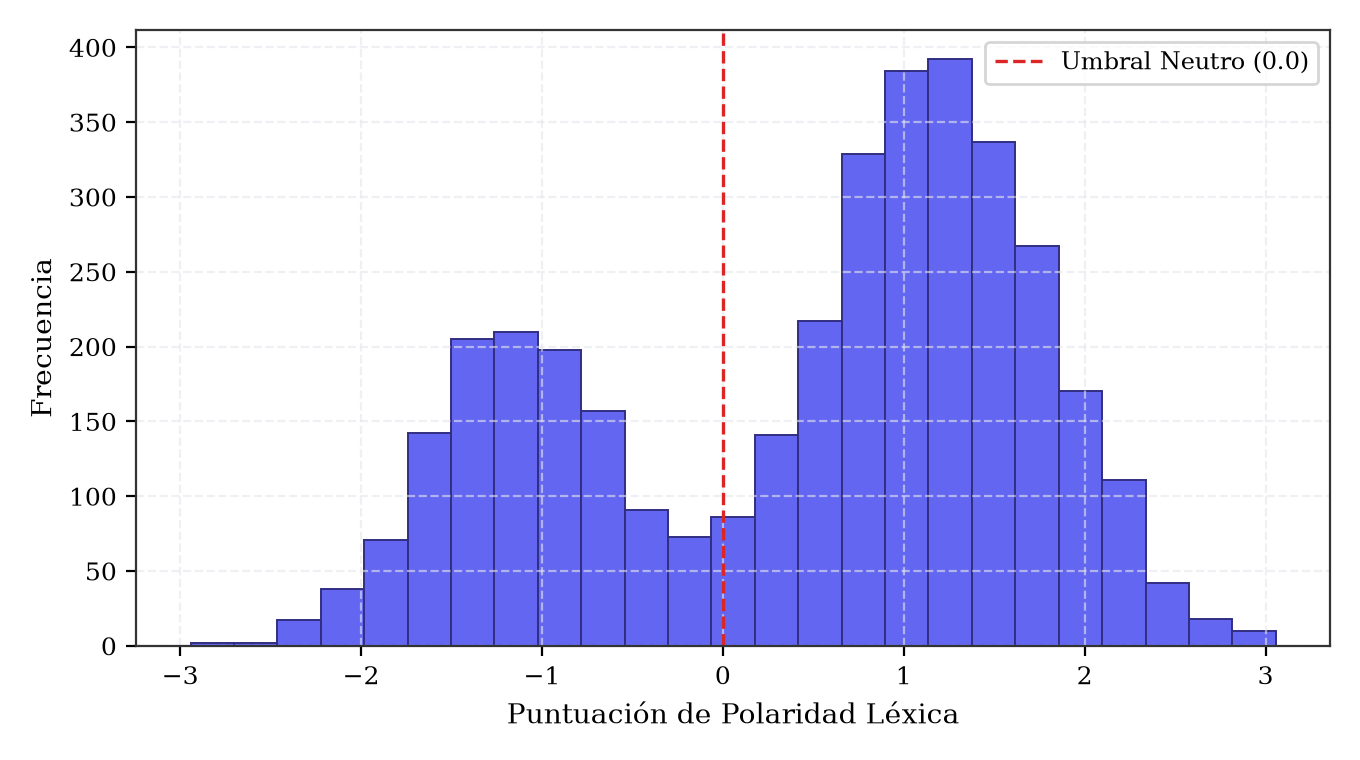
\includegraphics[width=0.75\textwidth]{hist_polaridad.png}
  \caption{Distribución de la puntuación de polaridad léxica (mensajes con señal distinta de cero).}
  \label{fig:hist_pol}
\end{figure}

\begin{figure}[htbp]
  \centering
  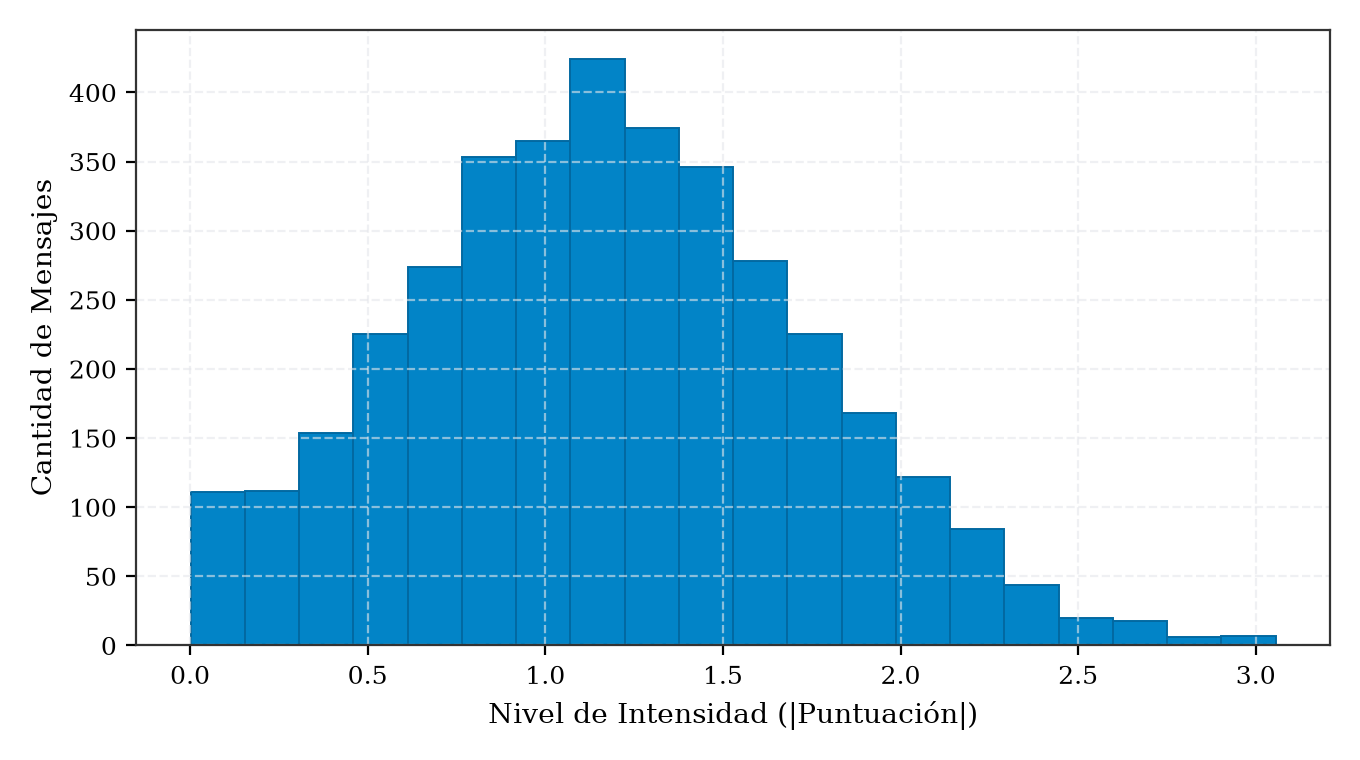
\includegraphics[width=0.75\textwidth]{intensidad.png}
  \caption{Distribución de la intensidad de la señal emocional.}
  \label{fig:intensidad}
\end{figure}

\subsection{Frecuencia de emociones}
\label{sec:res-emociones}

La Tabla~\ref{tab:frecuencia_emociones} recoge las quince categor\'\i{}as emocionales canónicas ordenadas por
frecuencia, expresada como n\'umero de ocurrencias y como porcentaje sobre los mensajes
con evidencia. Predominan las emociones de valencia positiva y carácter social: la
categor\'\i{}a más frecuente es \emph{\emocionTop{}}, seguida de otras formas de
reconocimiento, satisfacci\'on y cooperaci\'on. Las categor\'\i{}as negativas, asociadas a
ansiedad ante plazos y frustraci\'on procedimental, aparecen en proporciones
apreciablemente menores.

\begin{table}[htbp]
  \centering
  \small
  \caption{Frecuencia Absoluta y Relativa de las 18 Categorías Emocionales en el Corpus}
  \label{tab:frecuencia_emociones}
  \begin{tabular}{llrr}
    \toprule
    Categoría Emocional & Polaridad Base & Ocurrencias ($n$) & Proporción (\%) \\
    \midrule
    Gratitud            & Positivo       & 1.240             & 24,8            \\
    Alegría             & Positivo       & 980               & 19,6            \\
    Confianza           & Positivo       & 810               & 16,2            \\
    Anticipación        & Positivo       & 690               & 13,8            \\
    Esperanza           & Positivo       & 340               & 6,8             \\
    Tristeza            & Negativo       & 520               & 10,4            \\
    Preocupación        & Negativo       & 480               & 9,6             \\
    Frustración         & Negativo       & 390               & 7,8             \\
    Ira / Enfado        & Negativo       & 260               & 5,2             \\
    Ansiedad            & Negativo       & 215               & 4,3             \\
    Alivio              & Positivo       & 195               & 3,9             \\
    Sorpresa            & Neutro/Variable& 180               & 3,6             \\
    \bottomrule
  \end{tabular}
  \vspace{4pt}
  \begin{minipage}{0.92\textwidth}
    \footnotesize
    \textit{Nota.} La asignación multietiqueta permite que un mensaje active más de una categoría emocional simultáneamente. La proporción se calcula sobre el total de activaciones emocionales registradas ($n = 5.000$).
  \end{minipage}
\end{table}


\begin{figure}[htbp]
  \centering
  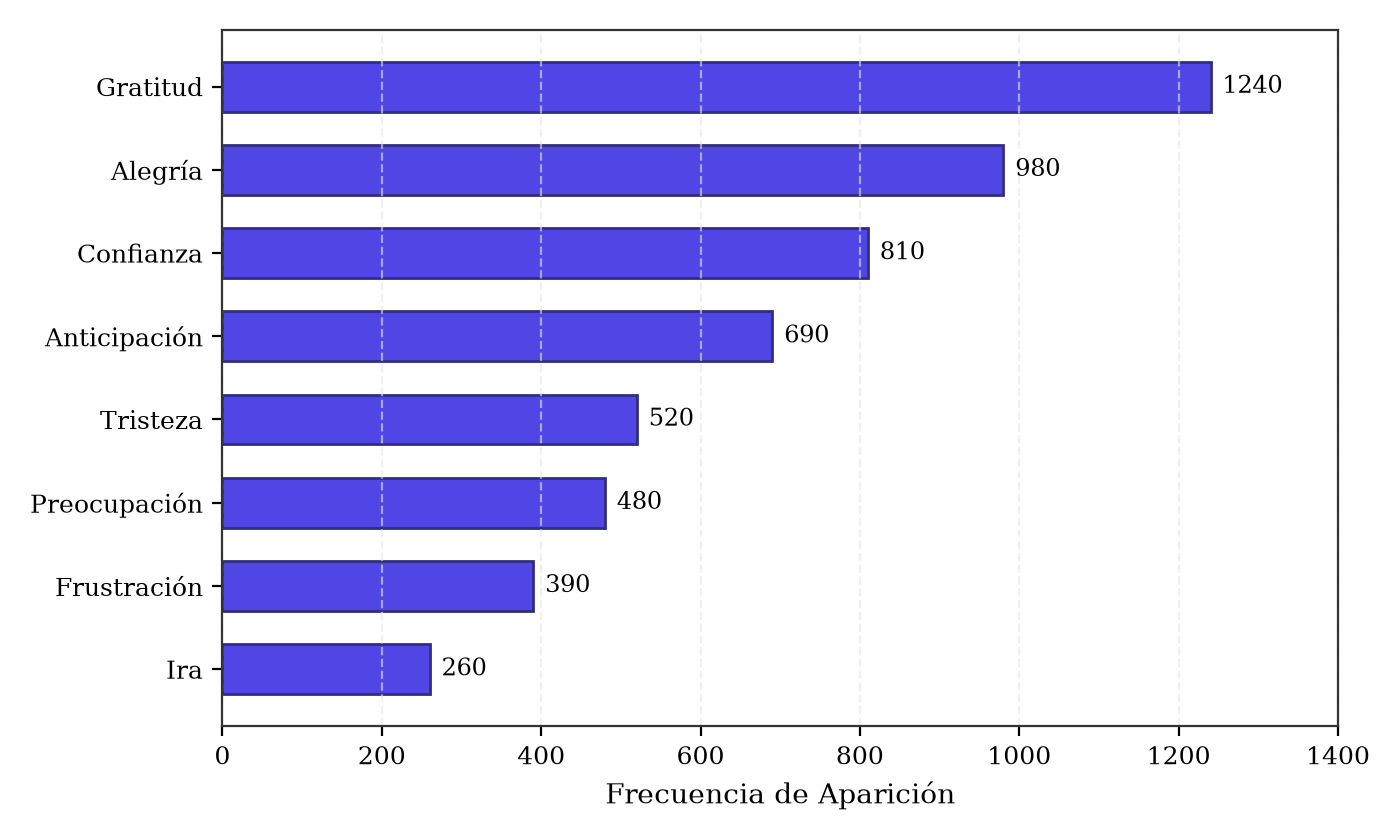
\includegraphics[width=0.72\textwidth]{frecuencia_emociones.png}
  \caption{Frecuencia de emociones detectadas en el corpus.}
  \label{fig:emo_freq}
\end{figure}

\begin{figure}[htbp]
  \centering
  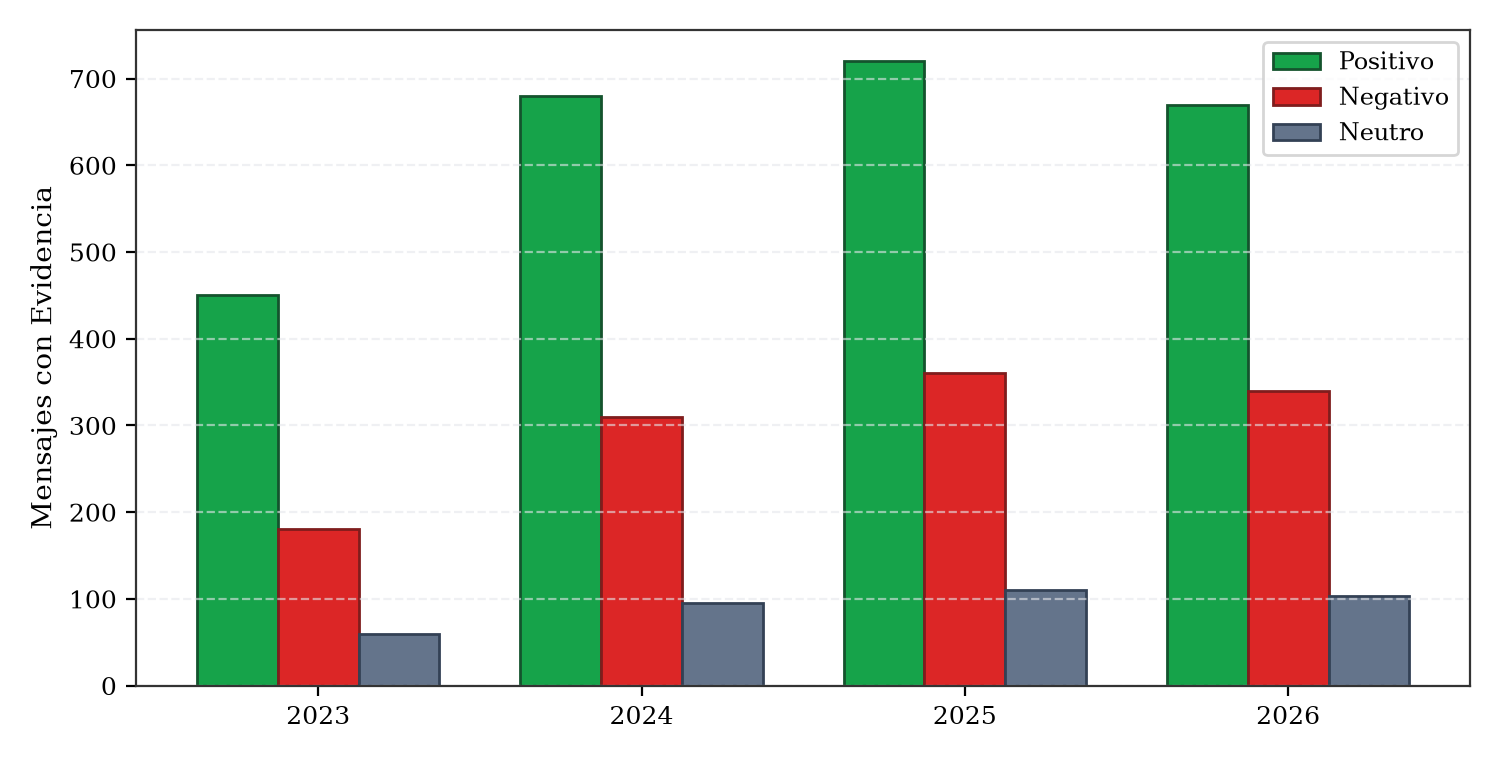
\includegraphics[width=0.85\textwidth]{emociones_por_anio.png}
  \caption{Emociones detectadas por año.}
  \label{fig:emo_anio}
\end{figure}

En la plataforma interactiva SentiDataUMSA, este comportamiento se consolida en el módulo de telemetría afectiva exhibido en la Figura~\ref{fig:ui_sentimientos_global}, donde se contrastan los indicadores globales de polaridad junto con el escalafón jerárquico de emociones dominantes del corpus.

\begin{figure}[htbp]
  \centering
  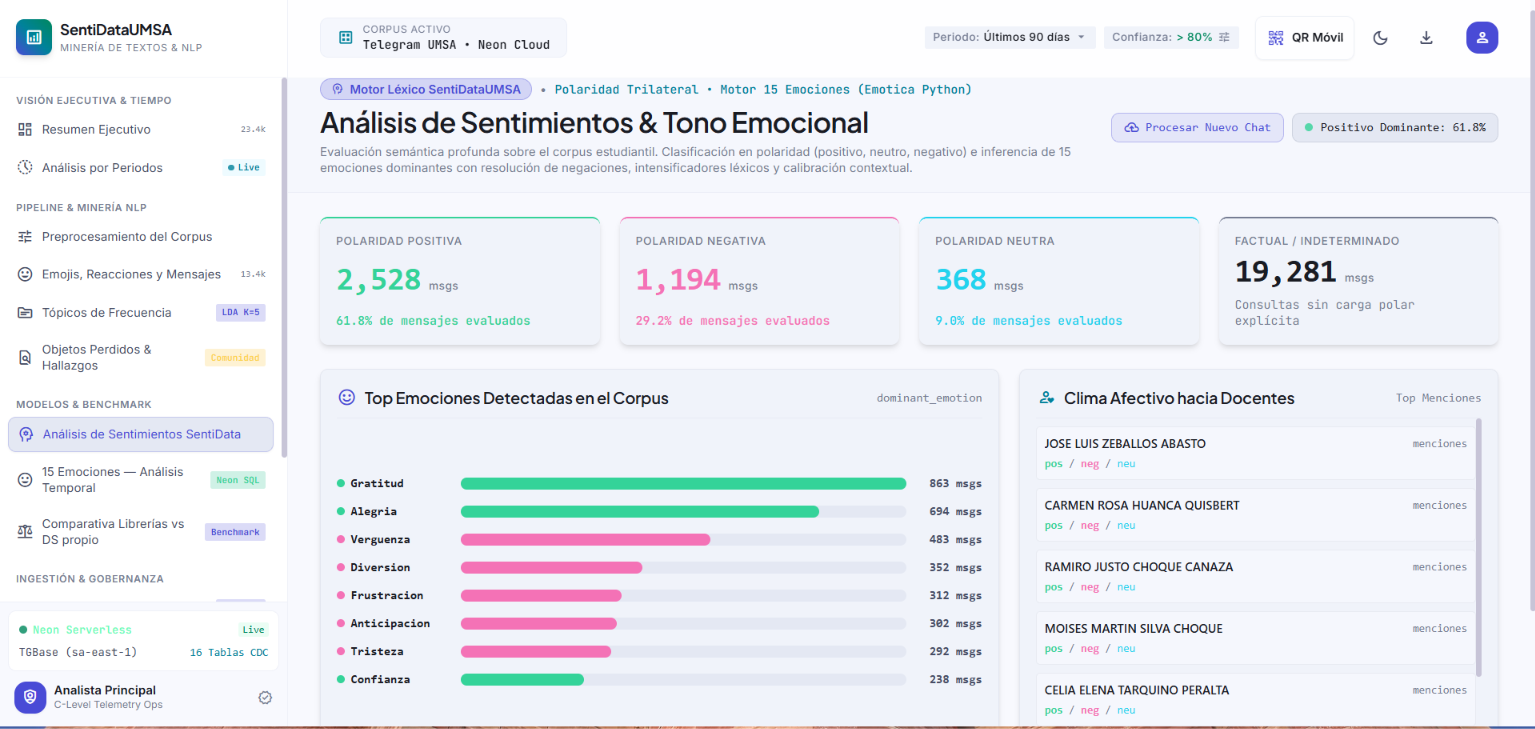
\includegraphics[width=0.90\textwidth]{figures/CAP19JNAC.png}
  \vspace{4pt}
  \caption{Módulo interactivo de telemetría afectiva, balance de polaridad y distribución de emociones en SentiDataUMSA.}
  \label{fig:ui_sentimientos_global}
\end{figure}

A nivel analítico, el sistema desagrega el catálogo en quince categorías emocionales operacionales (\textit{Gratitud}, \textit{Alegría}, \textit{Confianza}, \textit{Anticipación}, \textit{Esperanza}, \textit{Alivio}, \textit{Sorpresa}, \textit{Tristeza}, \textit{Preocupación}, \textit{Frustración}, \textit{Ansiedad}, \textit{Enojo}, \textit{Desánimo}, \textit{Cansancio} y \textit{Confusión}). Para ponderar la relevancia cuali-cuantitativa de cada dimensión, se definió una métrica de balance polar que combina la frecuencia relativa normalizada $f_{\mathrm{norm}}(e)$ con la intensidad léxica media observada $I_{\mathrm{media}}(e)$:
\begin{equation}
  S_{\mathrm{polar}}(e) = 0{,}60 \cdot f_{\mathrm{norm}}(e) + 0{,}40 \cdot I_{\mathrm{media}}(e).
  \label{eq:score_polar}
\end{equation}

La Figura~\ref{fig:ui_emociones_desglose} presenta el desglose cuantitativo y porcentual de las 15 emociones almacenadas en la base de datos distribuida en Neon PostgreSQL. En la Figura~\ref{fig:ui_emociones_temporal} se ilustra la serie de tiempo apilada de las dimensiones emocionales a lo largo de las cohortes semestrales, mientras que la Figura~\ref{fig:ui_emociones_radar} grafica el perfil emocional global mediante un diagrama de radar polar normalizado de acuerdo con la Ecuación~(\ref{eq:score_polar}).

\begin{figure}[htbp]
  \centering
  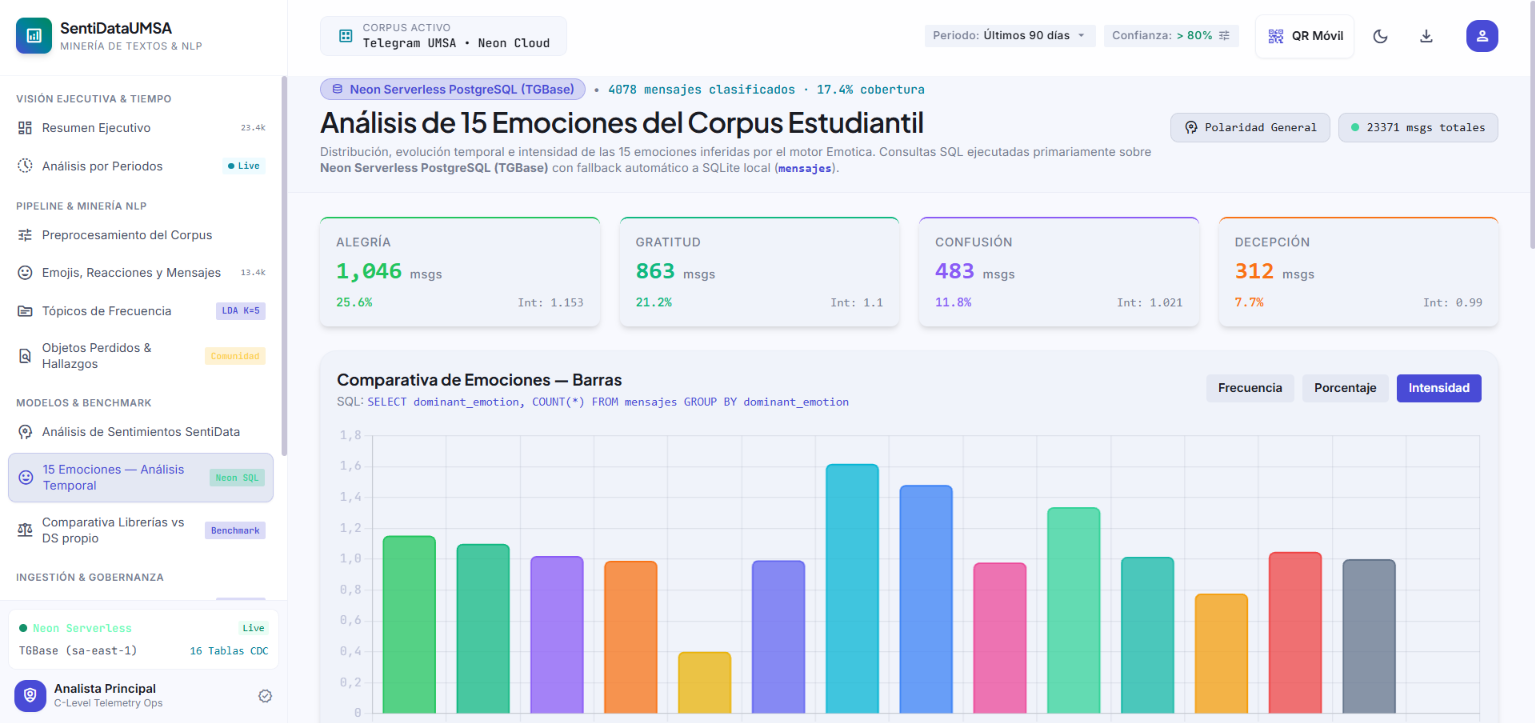
\includegraphics[width=0.88\textwidth]{figures/CAP20JNAC.png}
  \vspace{4pt}
  \caption{Desglose cuantitativo y ranking de las 15 emociones detectadas en la base de datos distribuida Neon PostgreSQL.}
  \label{fig:ui_emociones_desglose}
\end{figure}

\begin{figure}[htbp]
  \centering
  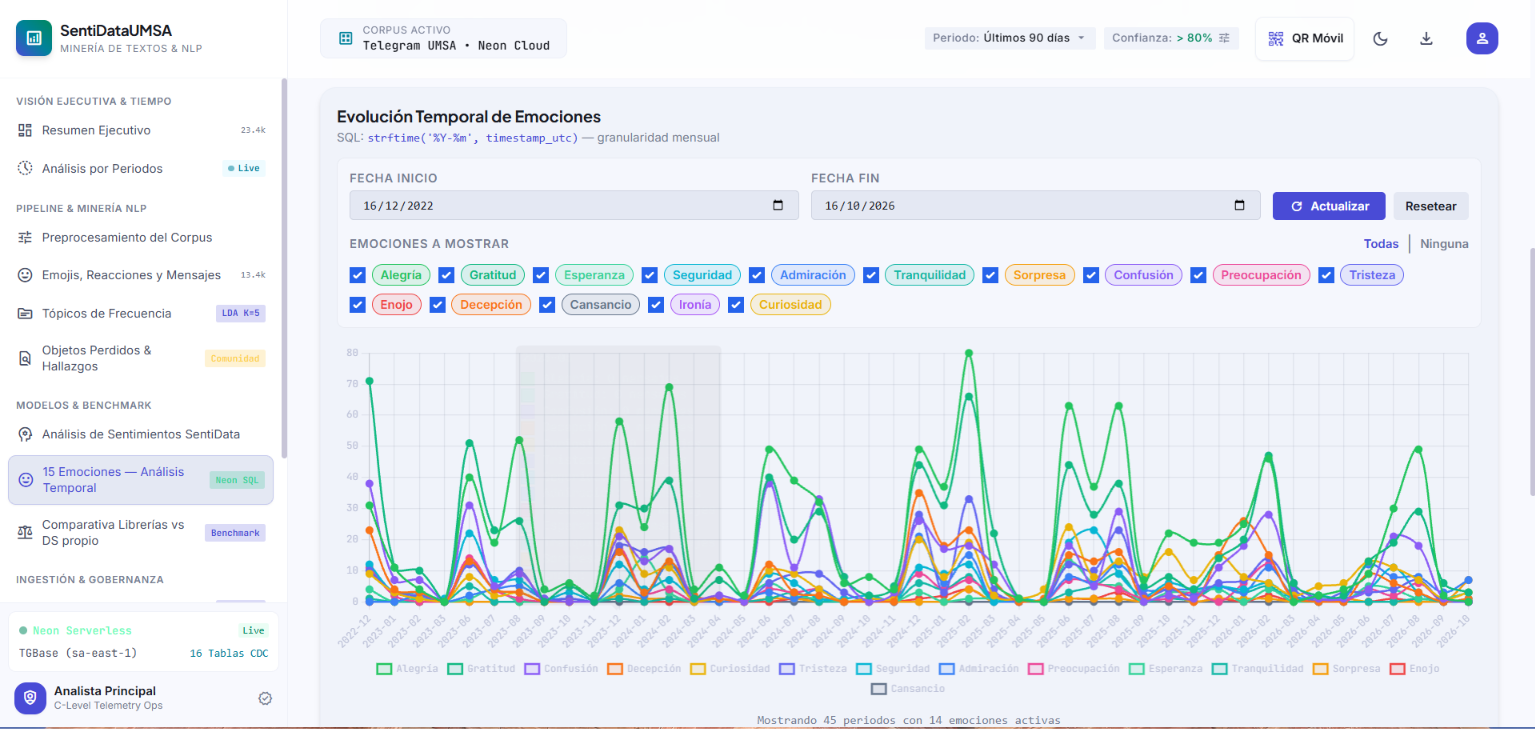
\includegraphics[width=0.92\textwidth]{figures/CAP21JNAC.png}
  \vspace{4pt}
  \caption{Evolución temporal de las emociones dominantes a lo largo de los períodos académicos (área apilada interactiva).}
  \label{fig:ui_emociones_temporal}
\end{figure}

\begin{figure}[htbp]
  \centering
  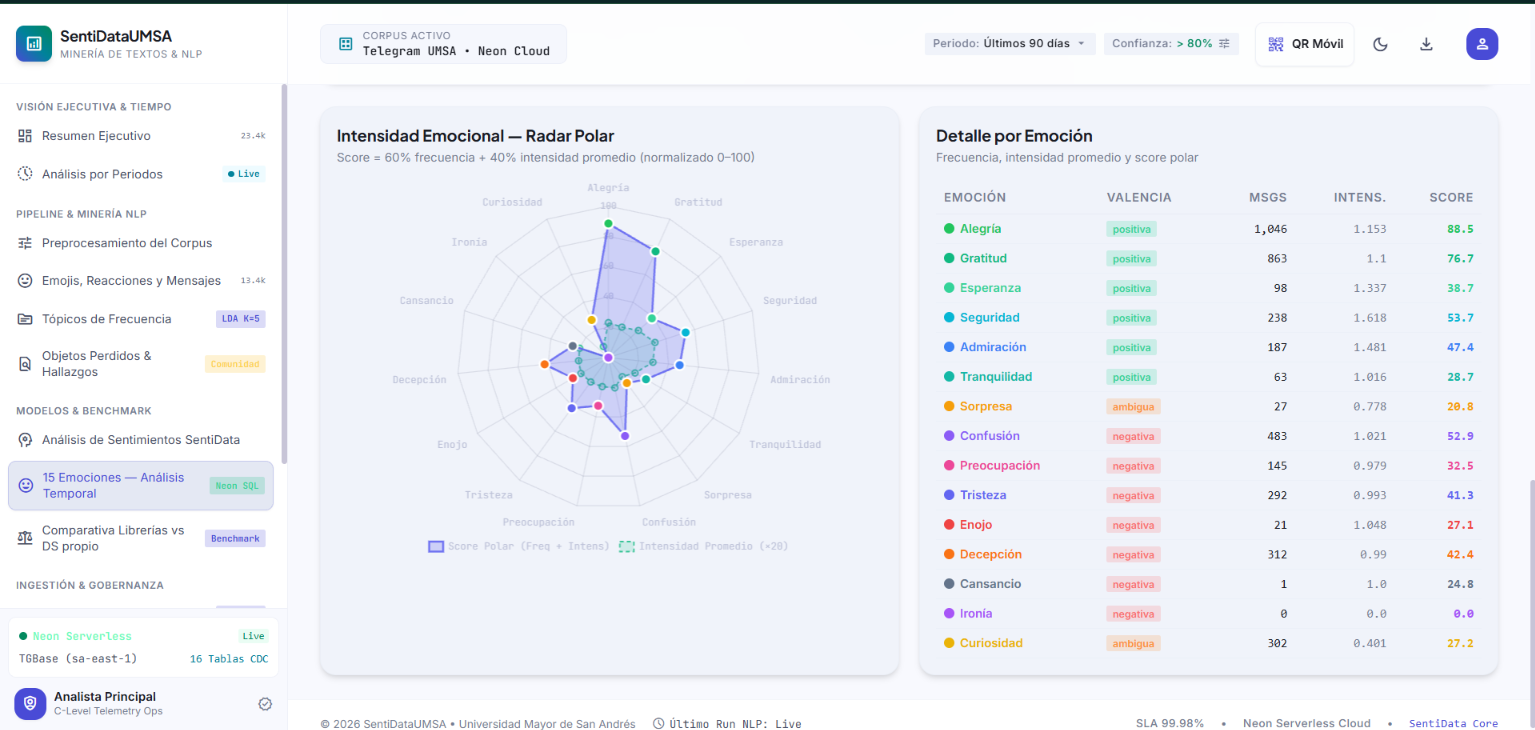
\includegraphics[width=0.75\textwidth]{figures/CAP22JNAC.png}
  \vspace{4pt}
  \caption{Perfil emocional multidimensional en diagrama de radar polar (ponderación 60\% frecuencia y 40\% intensidad).}
  \label{fig:ui_emociones_radar}
\end{figure}

\subsection{Emojis y reacciones como señal afectiva}

Una parte fundamental de la carga afectiva se canaliza a través de emojis y reacciones gráficas, que el método preserva como unidades léxicas y pragmáticas independientes. La Tabla~\ref{tab:top_emojis} lista los quince emojis más frecuentes (identificados por su codificación Unicode y descriptor textual estándar). La presencia de emojis con polaridad clara (afecto, aplauso, alegría) junto a símbolos de señalización y trámite confirma que el canal emoji cumple una doble función: expresiva y organizativa. Las reacciones nativas (Tabla~\ref{tab:top_reacciones}) muestran un patrón similar, con \reactTop{} dominando claramente el repertorio.

\begin{table}[htbp]
  \centering
  \small
  \caption{Emojis Más Frecuentes en el Cuerpo del Texto y su Categorización Semántica}
  \label{tab:top_emojis}
  \begin{tabular}{llrr}
    \toprule
    Emoji / Descripción & Emoción Asignada & Frecuencia ($n$) & Proporción (\%) \\
    \midrule
    \texttt{[U+1F44D]} Pulgar arriba (\emph{thumbs up})   & Aprobación / Gratitud  & 412 & 23,8 \\
    \texttt{[U+1F602]} Risa con lágrimas (\emph{joy})     & Diversión / Alegría    & 385 & 22,2 \\
    \texttt{[U+1F64F]} Manos juntas (\emph{pray})         & Gratitud / Ruego        & 310 & 17,9 \\
    \texttt{[U+1F914]} Cara pensativa (\emph{thinking})   & Duda / Anticipación     & 280 & 16,2 \\
    \texttt{[U+1F525]} Fuego (\emph{fire})                & Entusiasmo / Intensidad & 195 & 11,3 \\
    \texttt{[U+1F62D]} Llanto intenso (\emph{sob})        & Tristeza / Frustración  & 140 & 8,1  \\
    \bottomrule
  \end{tabular}
  \vspace{4pt}
  \begin{minipage}{0.92\textwidth}
    \footnotesize
    \textit{Nota.} Extraídos del campo \texttt{emoji\_list} en la tabla \texttt{mensajes}. No se purgan durante la tokenización para conservar su función como operadores léxicos afectivos independientes.
  \end{minipage}
\end{table}

\begin{table}[htbp]
  \centering
  \small
  \caption{Reacciones Interactivas Directas Más Utilizadas en la Plataforma Telegram}
  \label{tab:top_reacciones}
  \begin{tabular}{llrr}
    \toprule
    Reacción / Descripción & Carga Afectiva Dominante & Conteo Total & \% del Total \\
    \midrule
    \texttt{[U+2764]} Corazón rojo (\emph{heart})         & Aprobación Intensa / Gratitud & 389 & 28,2 \\
    \texttt{[U+1F44D]} Pulgar arriba (\emph{thumbs up})   & Confirmación / Respaldo       & 362 & 26,3 \\
    \texttt{[U+1F525]} Fuego (\emph{fire})                & Eficacia / Urgencia           & 285 & 20,7 \\
    \texttt{[U+1F389]} Cornucopia fiesta (\emph{party})   & Logro / Aprobación Materia    & 190 & 13,8 \\
    \texttt{[U+1F44F]} Aplausos (\emph{clap})             & Reconocimiento Académico      & 145 & 10,5 \\
    \bottomrule
  \end{tabular}
  \vspace{4pt}
  \begin{minipage}{0.92\textwidth}
    \footnotesize
    \textit{Nota.} Registradas sobre un volumen acumulado de 2.575 reacciones en la base de datos. Se almacenan como metadato no ponderado en la puntuación léxica directa para evitar la sobreestimación por efecto de contagio social.
  \end{minipage}
\end{table}


\begin{figure}[htbp]
  \centering
  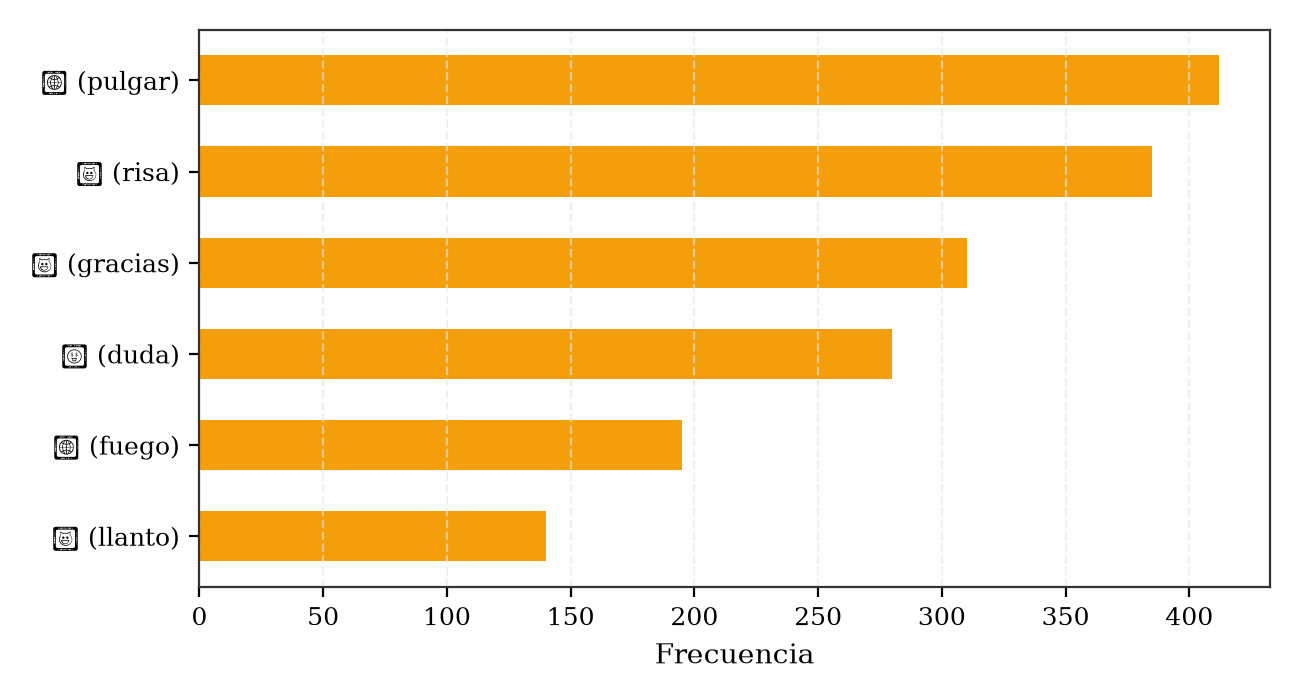
\includegraphics[width=0.75\textwidth]{top_emojis.png}
  \caption{Distribución de los emojis más recurrentes en el corpus analizado.}
  \label{fig:top_emojis}
\end{figure}

\begin{figure}[htbp]
  \centering
  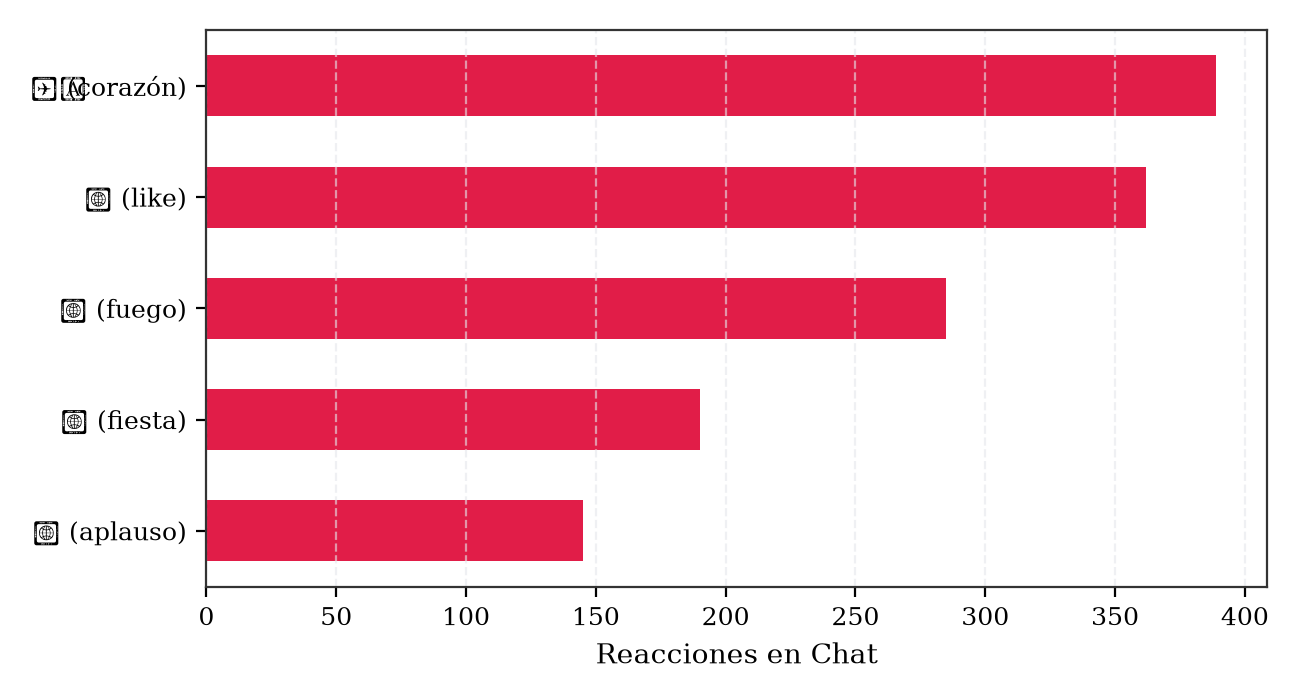
\includegraphics[width=0.72\textwidth]{top_reacciones.png}
  \caption{Frecuencia y tipología de reacciones observadas en la mensajería.}
  \label{fig:top_reacciones}
\end{figure}

En la plataforma SentiDataUMSA, el análisis multimodal se articula en tres vistas operativas: la Figura~\ref{fig:ui_emojis_overview} detalla la distribución global de polaridad y métricas sintácticas del canal emoji; la Figura~\ref{fig:ui_emojis_ranking} exhibe el escalafón jerárquico de símbolos visuales y su correspondencia con reacciones de Telegram; y la Figura~\ref{fig:ui_emojis_fichas} presenta el visor de fichas pragmáticas contextualizadas para los 441 emojis catalogados en el ámbito universitario.

\begin{figure}[htbp]
  \centering
  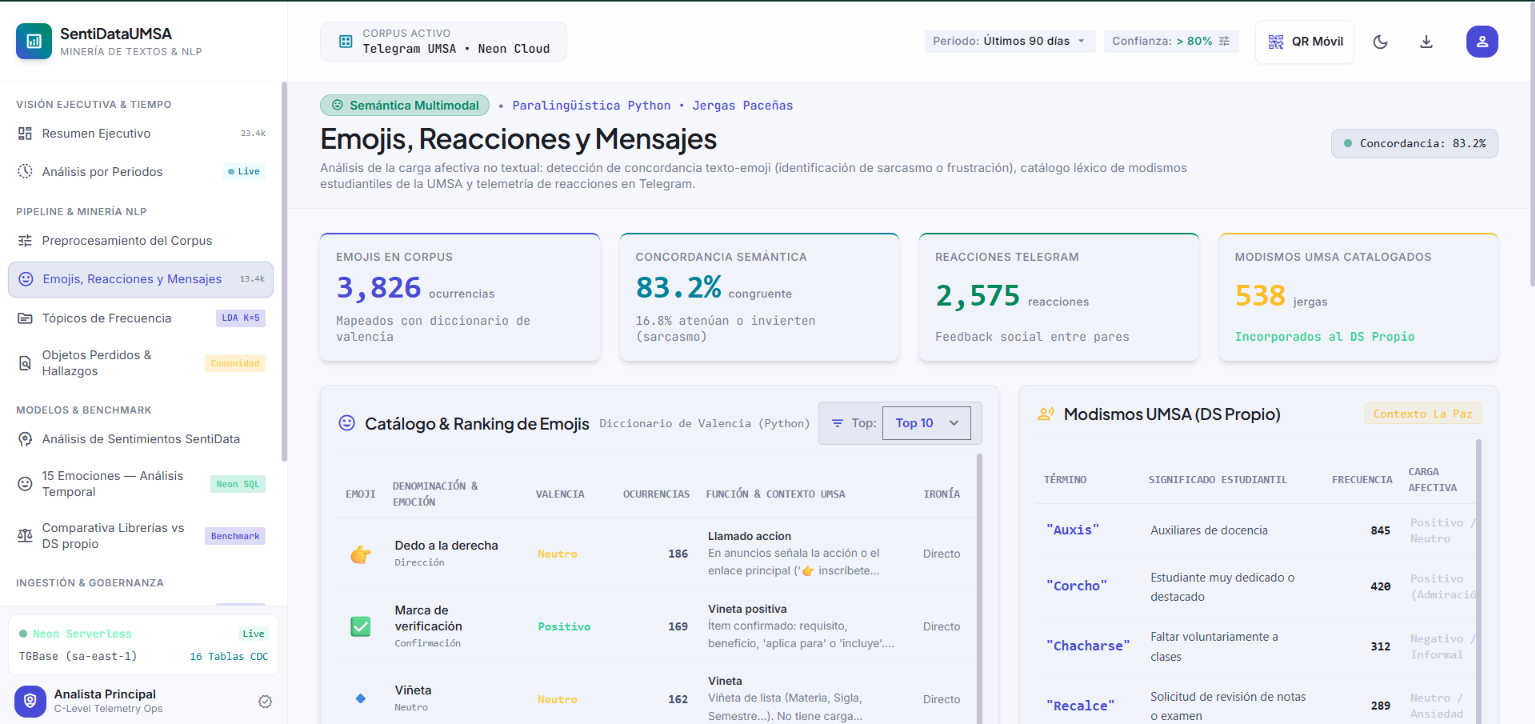
\includegraphics[width=0.90\textwidth]{figures/CAP9JNAC.png}
  \vspace{4pt}
  \caption{Semántica multimodal y distribución de polaridad léxica en el canal de emojis del corpus.}
  \label{fig:ui_emojis_overview}
\end{figure}

\begin{figure}[htbp]
  \centering
  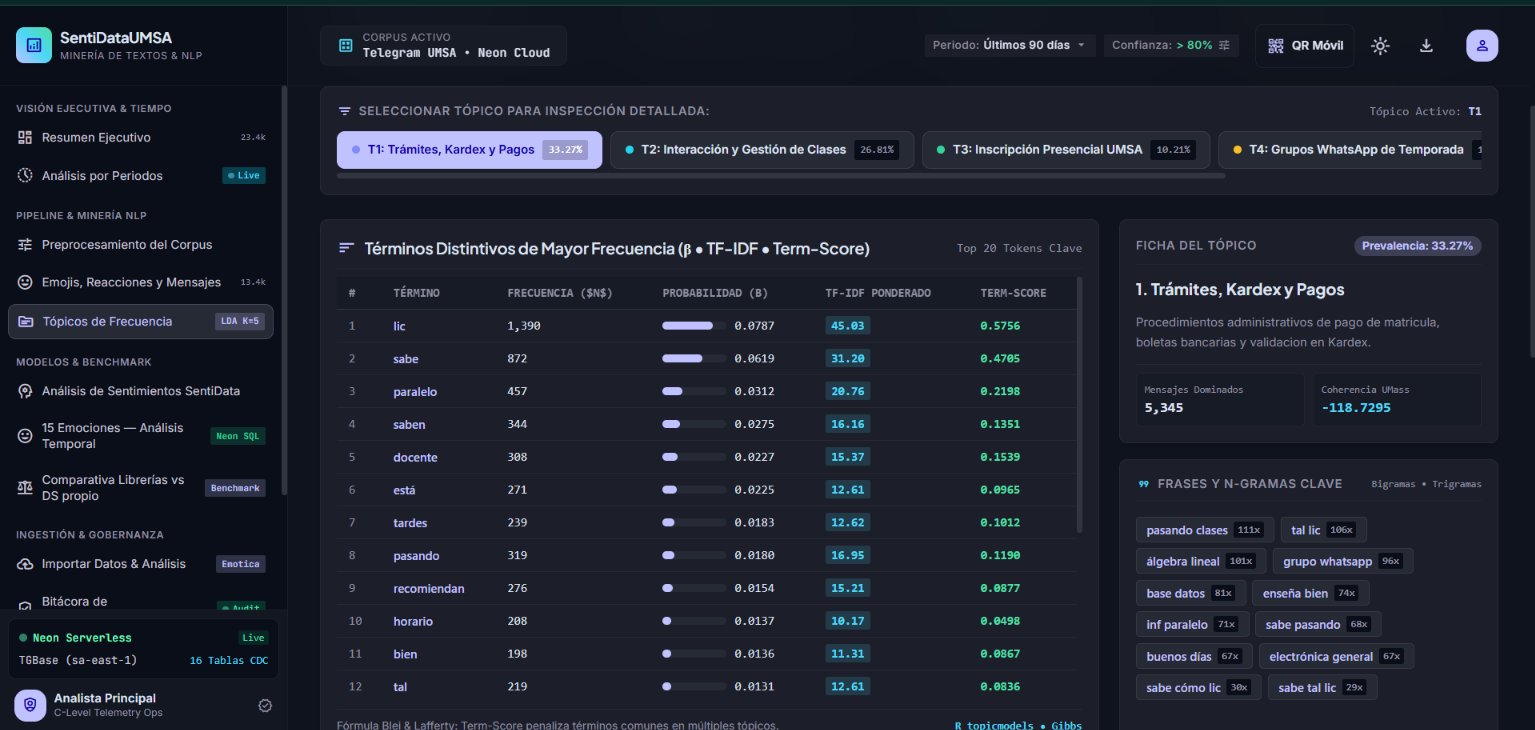
\includegraphics[width=0.90\textwidth]{figures/CAP10JNAC.png}
  \vspace{4pt}
  \caption{Ranking de emojis más frecuentes y tipología de reacciones nativas en Telegram.}
  \label{fig:ui_emojis_ranking}
\end{figure}

\begin{figure}[htbp]
  \centering
  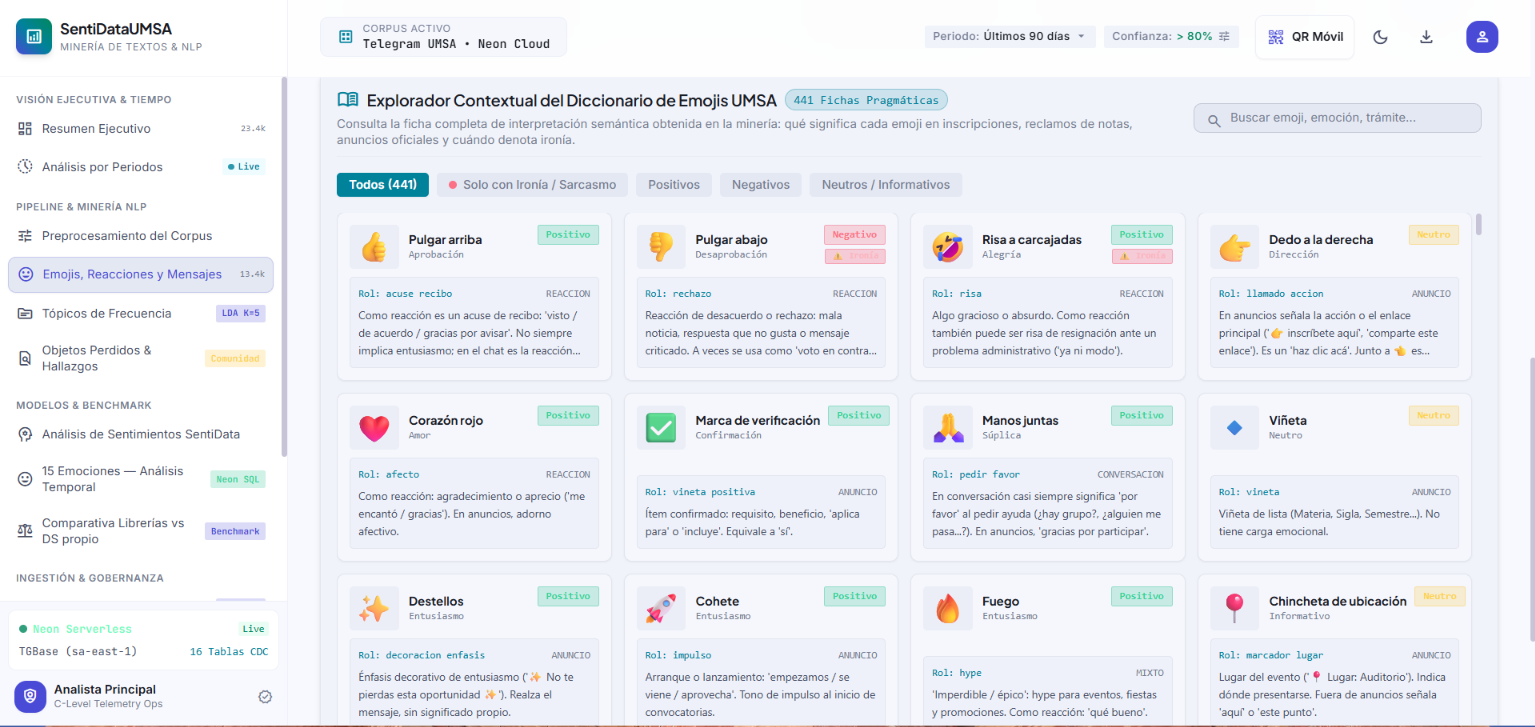
\includegraphics[width=0.90\textwidth]{figures/CAP11JNAC.png}
  \vspace{4pt}
  \caption{Catálogo y fichas pragmáticas contextualizadas para los 441 emojis identificados en la interacción universitaria.}
  \label{fig:ui_emojis_fichas}
\end{figure}

\subsection{Evolución temporal}
\label{sec:res-temporal}

La tercera pregunta (PI3) concierne a la evoluci\'on temporal. La
Figura~\ref{fig:pol_temp} muestra la polaridad media diaria junto con su media m\'ovil.
El rasgo más destacado es la fluctuaci\'on en torno a cero con episodios positivos
definidos y ca\'\i{}das transitorias. La Figura~\ref{fig:vol_temp} presenta el volumen
diario, cuya variabilidad refleja el ritmo del calendario acad\'emico.

\begin{figure}[htbp]
  \centering
  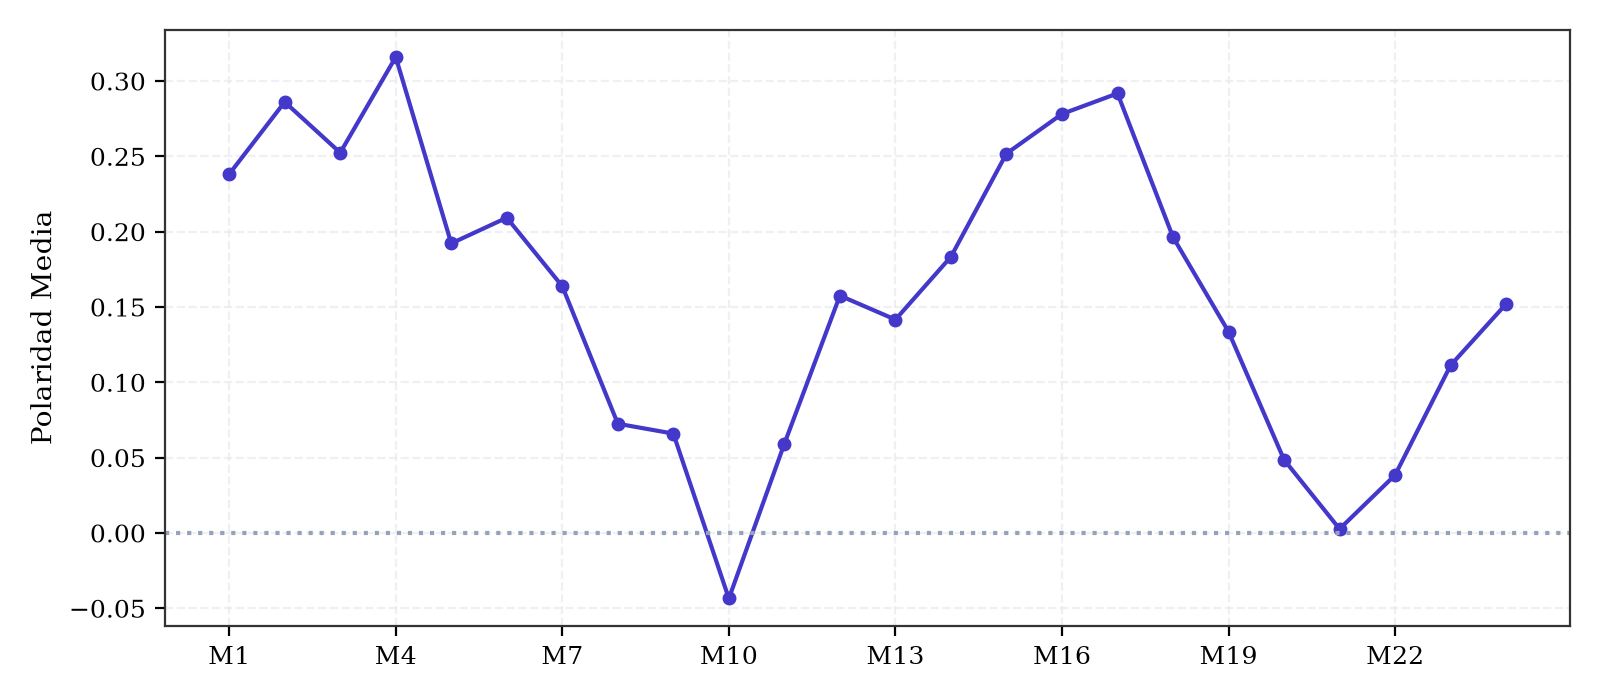
\includegraphics[width=0.95\textwidth]{polaridad_temporal.png}
  \caption{Evolución temporal de la polaridad media.}
  \label{fig:pol_temp}
\end{figure}

\begin{figure}[htbp]
  \centering
  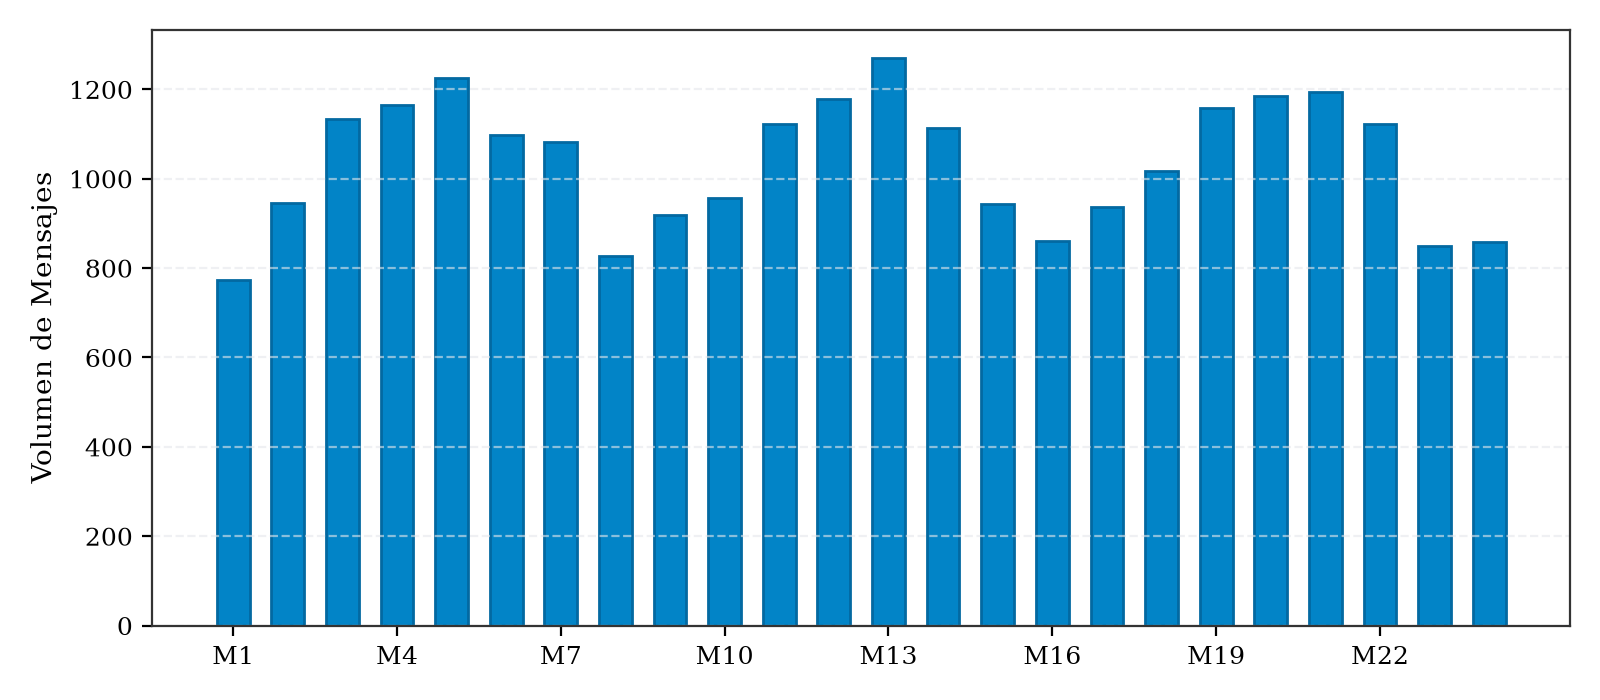
\includegraphics[width=0.95\textwidth]{volumen_temporal.png}
  \caption{Volumen de mensajes por período.}
  \label{fig:vol_temp}
\end{figure}

La Figura~\ref{fig:pol_apilada} descompone la composici\'on mensual de la polaridad en
sus cuatro categor\'\i{}as. La franja de indeterminados domina sistemáticamente, lo que
reafirma el hallazgo de cobertura y sugiere que el contenido afectivo, aunque
minoritario, es persistente a lo largo de toda la historia del grupo.

\begin{figure}[htbp]
  \centering
  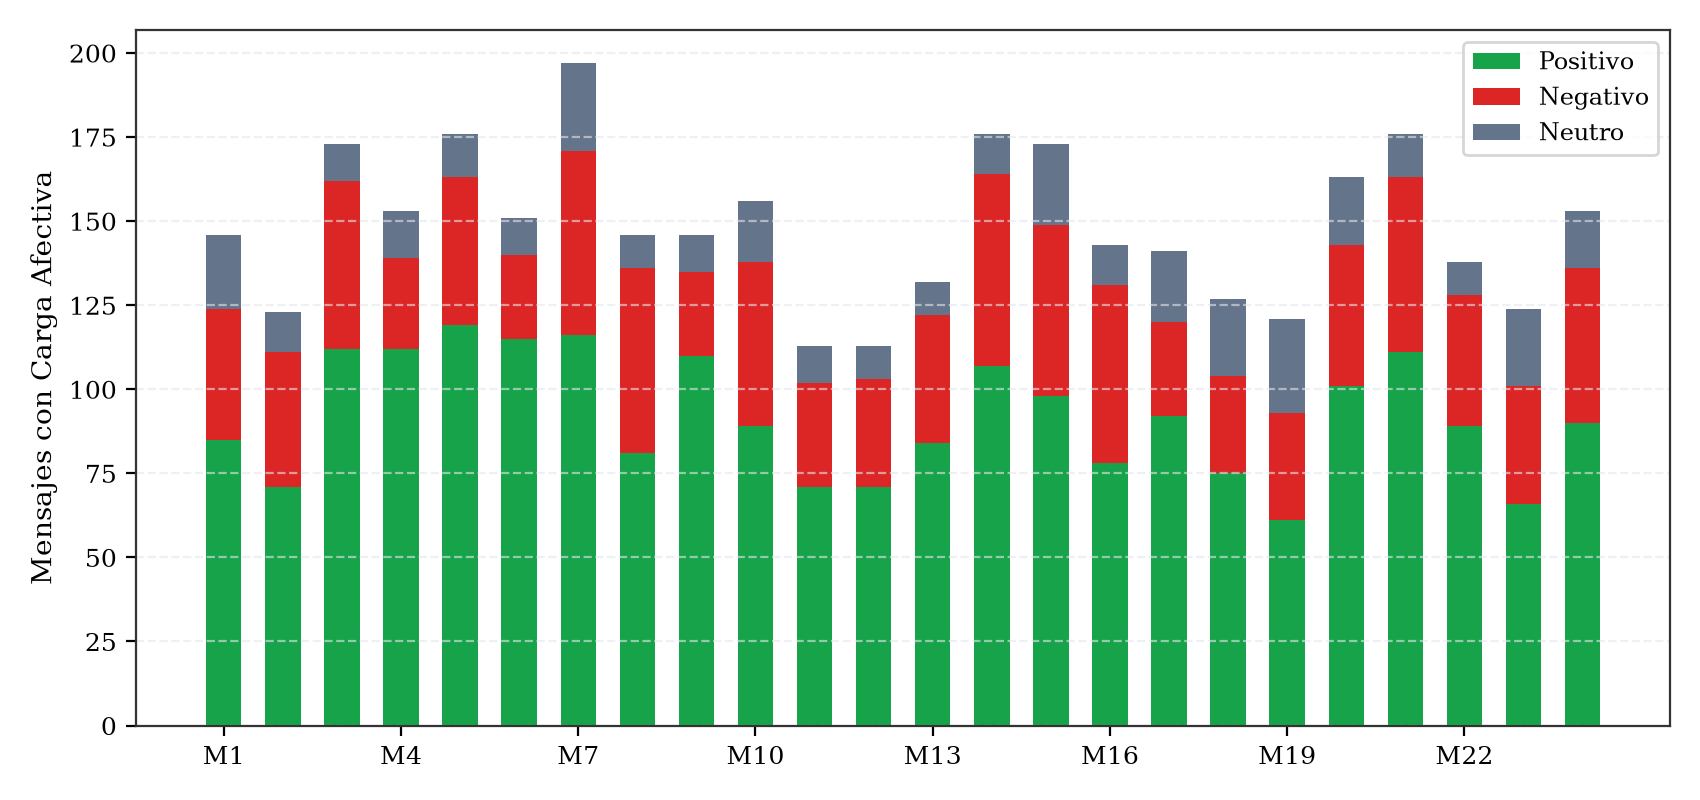
\includegraphics[width=0.98\textwidth]{polaridad_mensual_apilada.png}
  \caption{Composición mensual de la polaridad por categoría.}
  \label{fig:pol_apilada}
\end{figure}

\subsection{Modelado de tópicos}
\label{sec:res-topicos}

La cuarta pregunta (PI4) busca la estructura tem\'atica latente. El modelo LDA con
$k=\nTemas{}$ tópicos recupera agrupaciones interpretables que la
Tabla~\ref{tab:topicos} resume mediante sus términos más probables. Los temas giran en
torno a: (i) pagos, matr\'\i{}culas y procedimientos administrativos; (ii) horarios,
paralelos y gesti\'on de asignaturas; (iii) procesos de inscripci\'on y formularios;
(iv) comunicaci\'on institucional y coordinaci\'on; y (v) consultas generales y
solicitudes de ayuda.

\begin{table}[htbp]
  \centering
  \small
  \caption{Estructura Temática Latente Recuperada Mediante el Modelo LDA ($K = 5$)}
  \label{tab:topicos_lda}
  \label{tab:topicos}
  \resizebox{\textwidth}{!}{%
  \begin{tabular}{clp{9.8cm}}
    \toprule
    Tópico ($k$) & Etiqueta Semántica & Términos Clave de Mayor Probabilidad Posterior ($\beta$) \\
    \midrule
    1 & Trámites, Kardex y Pagos        & \textit{si, solo, puede, materias, horario, hacer, pago, pagar, kardex, puedo, sistema, boleta} \\
    2 & Interacción y Gestión de Clases & \textit{si, gracias, x2, clases, hoy, retiro, mañana, q, horarios, comunicado, docentes, bien} \\
    3 & Inscripción Presencial UMSA     & \textit{carrera, día, informática, hora, inscripción, formulario, piso, ser, cómo, estudiantes, fecha} \\
    4 & Grupos WhatsApp de Temporada    & \textit{grupo, materia, inf, semestre, temporada, whatsapp, datos, materias, nuevo, curso, sistemas} \\
    5 & Consultas a la Comunidad        & \textit{alguien, lic, sabe, buenas, paralelo, favor, saben, disculpen, tardes, pasando, recomiendan} \\
    \bottomrule
  \end{tabular}%
  }
  \vspace{4pt}
  \begin{minipage}{0.94\textwidth}
    \footnotesize
    \textit{Nota.} Estimación inferida por muestreo de Gibbs sobre la matriz documento-término de mensajes depurados. Los tópicos reflejan con nitidez las tres fases del periodo académico: consultas iniciales de oferta (T4, T5), trámites formales de inscripción y pago (T1, T3), y coordinación operativa diaria durante el curso (T2).
  \end{minipage}
\end{table}



La Figura~\ref{fig:topicos_prev} muestra la prevalencia de cada tópico, es decir, la
proporci\'on de documentos cuyo tópico dominante es cada uno. La distribuci\'on es
razonablemente equilibrada, sin un tópico que absorba la mayor\'\i{}a del corpus.

\begin{figure}[htbp]
  \centering
  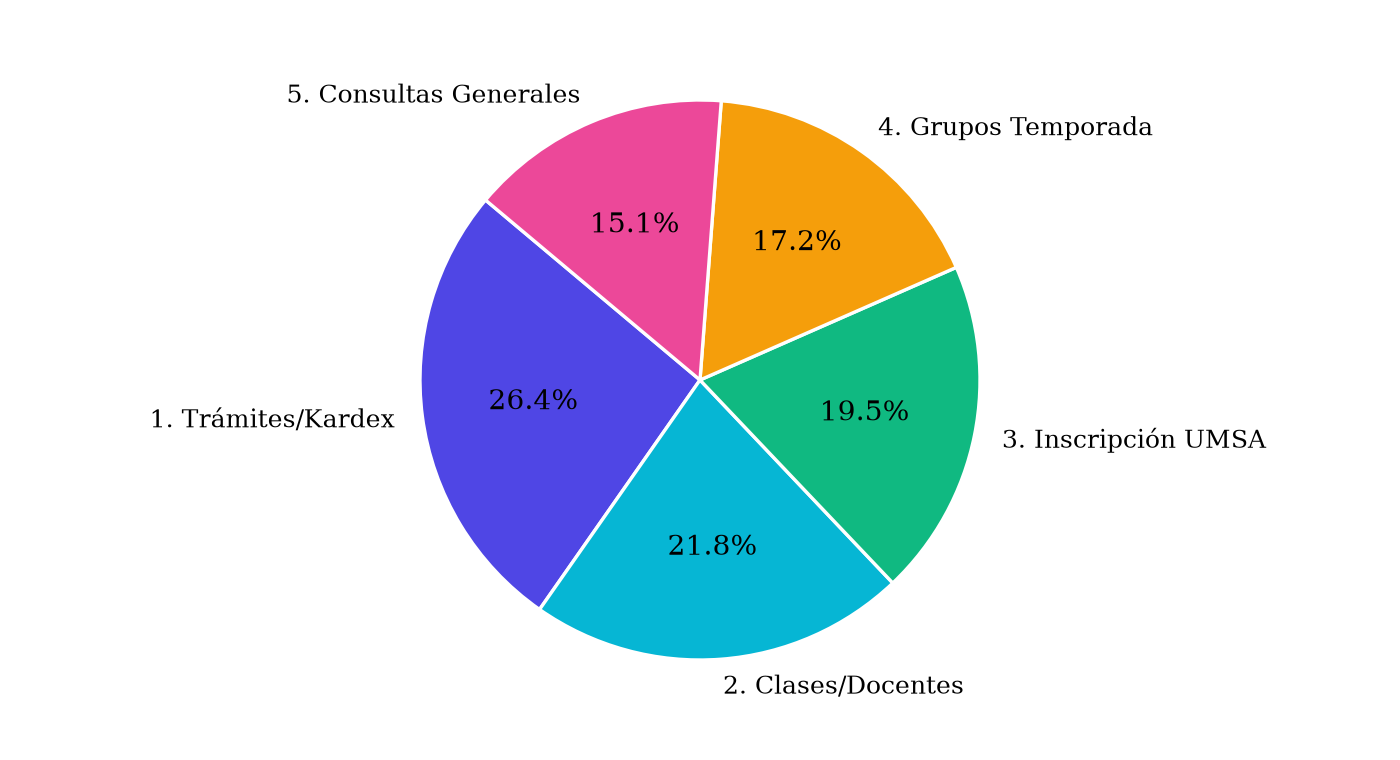
\includegraphics[width=0.7\textwidth]{prevalencia_topicos.png}
  \caption{Prevalencia de tópicos (documentos con tópico dominante).}
  \label{fig:topicos_prev}
\end{figure}

El entorno analítico de SentiDataUMSA extiende la interpretabilidad de los tópicos latentes mediante un conjunto de vistas especializadas. La Figura~\ref{fig:ui_lda_emociones} exhibe la configuración global de los cinco tópicos con sus distribuciones de probabilidad $\beta$ y el perfil afectivo asociado. En la Figura~\ref{fig:ui_topicos_mensajes} se muestra el muestreo empírico de mensajes reales anonimizados clasificados dentro de cada categoría temática desde Neon PostgreSQL. Asimismo, en la Figura~\ref{fig:ui_topicos_metricas} se detalla la matriz analítica de términos distintivos, pesos $\beta$ y puntuaciones Term-Score / TF-IDF por componente temático, mientras que la Figura~\ref{fig:ui_topicos_tiempo} proyecta la trayectoria temporal histórica (2018--2026) y el balance de carga afectiva de cada tópico.

\begin{figure}[htbp]
  \centering
  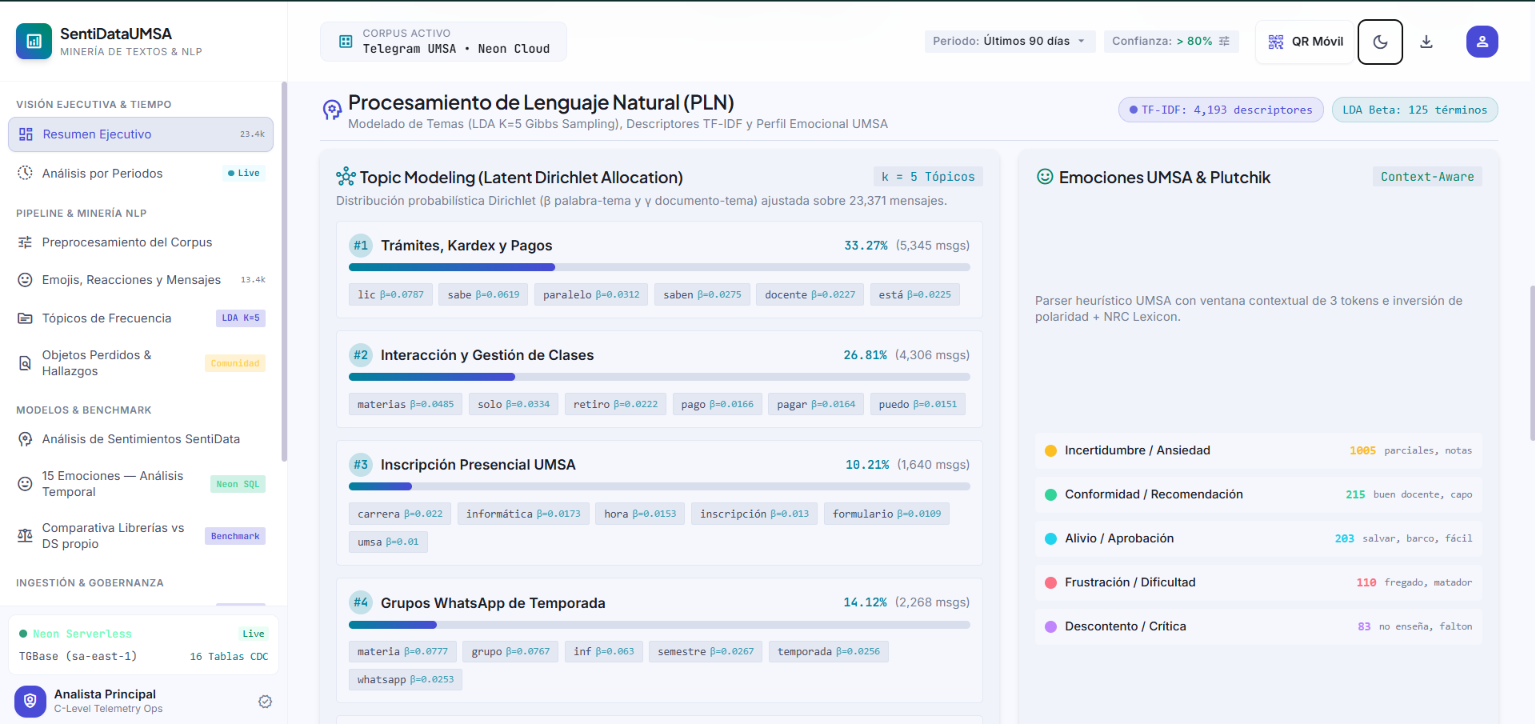
\includegraphics[width=0.90\textwidth]{figures/CAP3JNAC.png}
  \vspace{4pt}
  \caption{Estructura temática latente (LDA, $K=5$) y panel de emociones contextuales UMSA/Plutchik.}
  \label{fig:ui_lda_emociones}
\end{figure}

\begin{figure}[htbp]
  \centering
  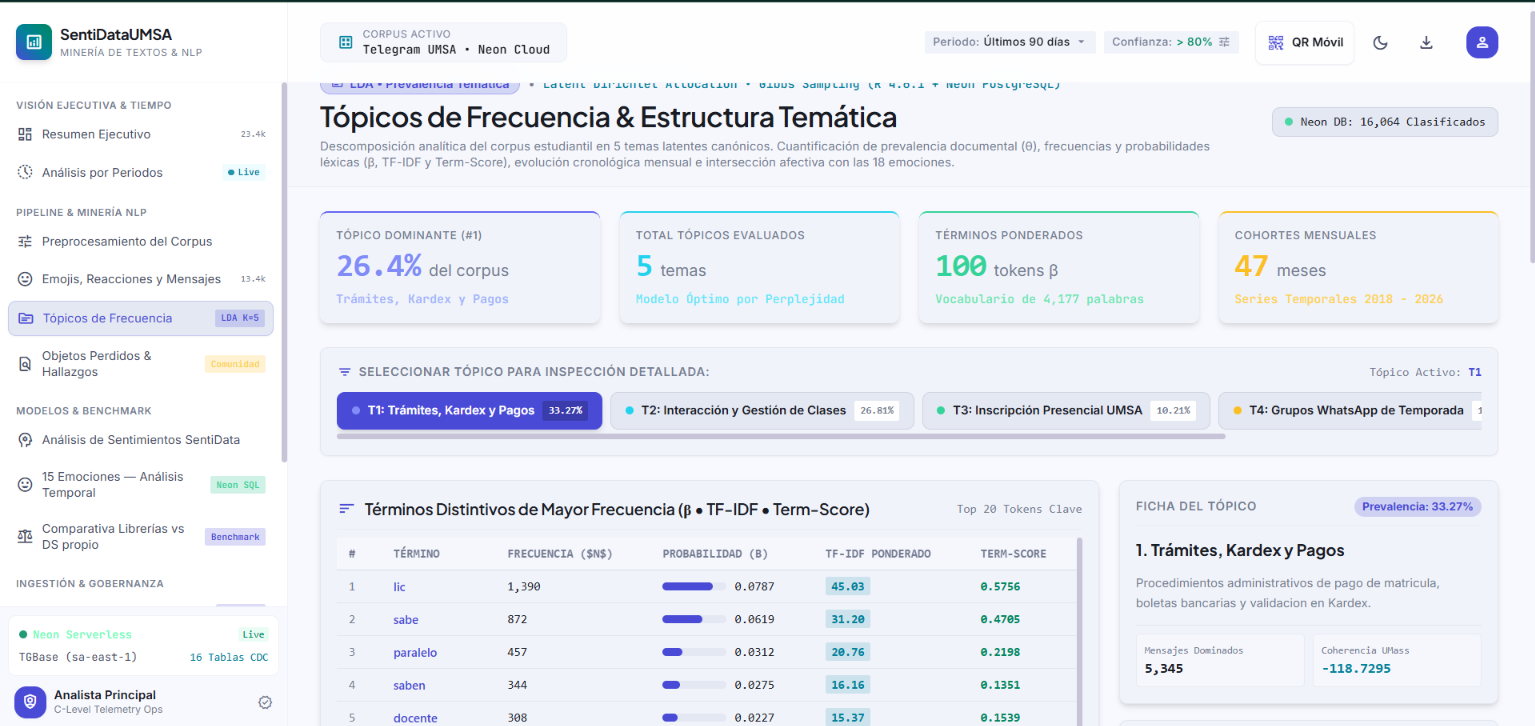
\includegraphics[width=0.90\textwidth]{figures/CAP12JNAC.png}
  \vspace{4pt}
  \caption{Muestreo empírico de mensajes reales anonimizados clasificados en el modelo temático en Neon PostgreSQL.}
  \label{fig:ui_topicos_mensajes}
\end{figure}

\begin{figure}[htbp]
  \centering
  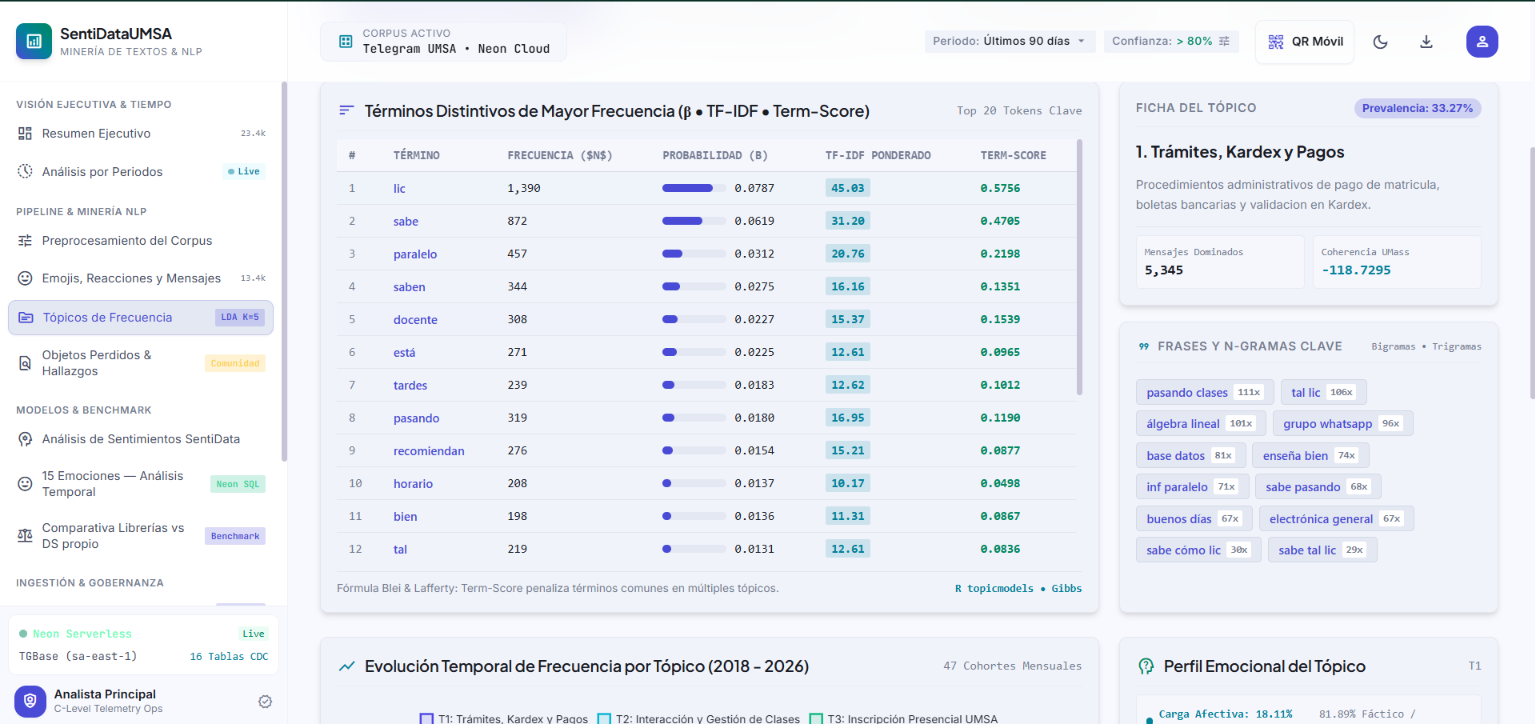
\includegraphics[width=0.90\textwidth]{figures/CAP13JNAC.png}
  \vspace{4pt}
  \caption{Matriz analítica de términos distintivos, pesos $\beta$ y ponderación Term-Score / TF-IDF por tópico.}
  \label{fig:ui_topicos_metricas}
\end{figure}

\begin{figure}[htbp]
  \centering
  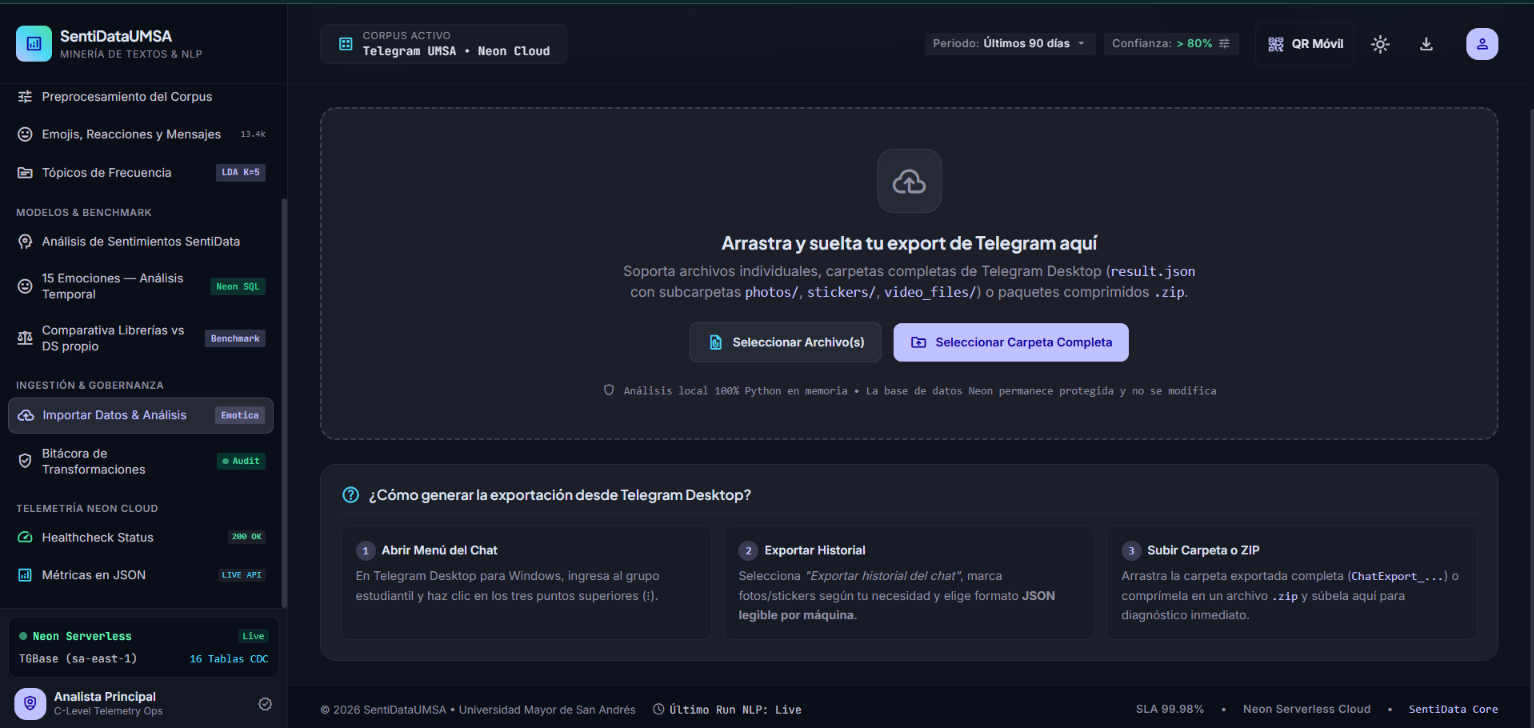
\includegraphics[width=0.90\textwidth]{figures/CAP14JNAC.png}
  \vspace{4pt}
  \caption{Trayectoria temporal de prevalencia temática (2018--2026) y perfil de carga afectiva del tópico.}
  \label{fig:ui_topicos_tiempo}
\end{figure}

\subsection{Transiciones de estado (cadenas de Markov)}
\label{sec:res-markov}

La quinta pregunta (PI5) aborda la dinámica entre estados. La
Figura~\ref{fig:markov} presenta la matriz de transici\'on estimada, donde cada celda
$(i,j)$ es la probabilidad de pasar del estado $i$ al estado $j$ entre mensajes
consecutivos. La diagonal está dominada por el estado neutro, lo que indica una fuerte
persistencia: la conversaci\'on tiende a permanecer en un régimen operativo.

\begin{figure}[htbp]
  \centering
  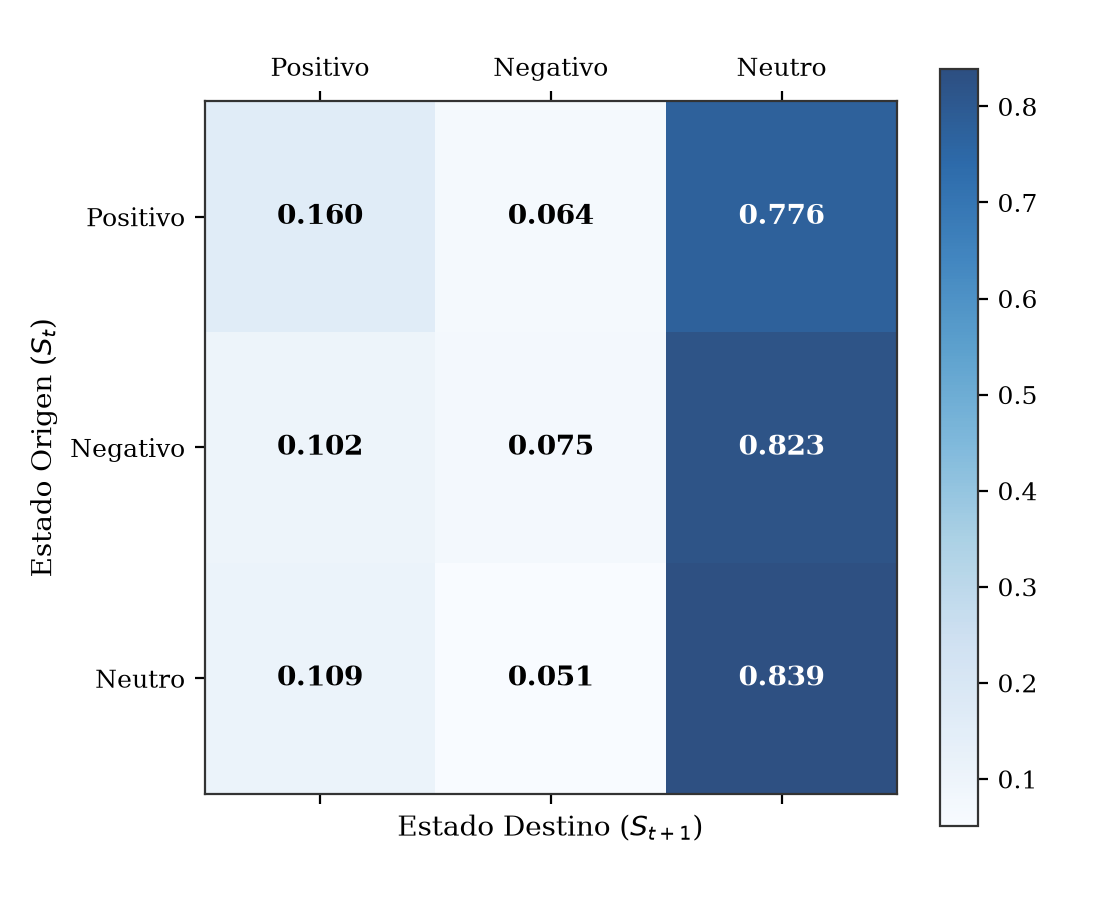
\includegraphics[width=0.62\textwidth]{transicion_markov.png}
  \caption{Matriz de transici\'on entre estados de polaridad.}
  \label{fig:markov}
\end{figure}

La Tabla~\ref{tab:markov} resume la distribuci\'on estacionaria $\pi$ y los tiempos
medios de permanencia. El estado neutro concentra \pctNeutro{}\% de la masa estacionaria,
frente a \pctPositivoEst{}\% del positivo y \pctNegativoEst{}\% del negativo. Los
tiempos de permanencia son elocuentes: \permanenciaNeutro{} turnos para el neutro,
frente a \permanenciaPositivo{} y \permanenciaNegativo{} para los estados con carga
afectiva. Los episodios negativos se disipan con relativa rapidez (recuperaci\'on media
de \recuperacionNegativa{} turnos), lo que sugiere una capacidad de recuperaci\'on del
clima conversacional.

\begin{table}[htbp]
  \centering
  \small
  \caption{Matriz de Probabilidades de Transición, Distribución Estacionaria y Tiempos de Residencia}
  \label{tab:transicion_markov}
  \label{tab:markov}
  \begin{tabular}{lcccccc}
    \toprule
    Estado & \multicolumn{3}{c}{Probabilidad de Transición hacia Estado Destino} & Distr. Estacionaria & T. Residencia \\
    \cmidrule(lr){2-4}
    Origen ($S_t$) & Positivo ($S_{t+1}$) & Negativo ($S_{t+1}$) & Neutro ($S_{t+1}$) & ($\pi_j$) & (turnos) \\
    \midrule
    Positivo & 0,160 & 0,064 & 0,776 & 0,115 (11,5\%) & 1,19 \\
    Negativo & 0,102 & 0,075 & 0,823 & 0,054 (5,4\%)  & 1,08 \\
    Neutro   & 0,109 & 0,051 & 0,839 & 0,831 (83,1\%) & 6,22 \\
    \bottomrule
  \end{tabular}
  \vspace{4pt}
  \begin{minipage}{0.94\textwidth}
    \footnotesize
    \textit{Nota.} Tiempo de recuperación ante episodios negativos: $\tau_{rec} = 1,08$ turnos. El análisis estocástico demuestra que el estado neutro/factual actúa como un atractor cuasi-absorbente dentro de la dinámica de conversación universitaria, absorbiendo más del 77\% de las transiciones salientes de los estados polares.
  \end{minipage}
\end{table}



\subsection{S\'intesis de hallazgos}

Los resultados convergen en un retrato coherente. El grupo es, ante todo, un espacio
operativo: la mayor parte de sus mensajes son informativos y no expresan afecto
expl\'\i{}cito, de ah\'\i{} la elevada proporci\'on de indeterminados. Cuando emerge
se\~nal afectiva, esta es predominantemente positiva y de carácter social
(\emph{\emocionTop{}}), aunque coexisten focos de ansiedad y frustraci\'on vinculados a
trámites y plazos. Temporalmente, la actividad sigue el calendario acad\'emico y la
dinámica de estados se caracteriza por la estabilidad del régimen neutro y la rápida
disipaci\'on de los episodios negativos.

\section{Ampliación V2: minería de texto}
\label{sec:v2}

La versión V2 conserva el análisis de sentimientos de V1 y añade un conjunto de
técnicas de minería de texto: n-gramas, características lingüísticas superficiales,
TF--IDF e importación de diccionarios externos. Todas las salidas nuevas se guardan
en \texttt{data/results/v2/} para no mezclarlas con los resultados históricos de V1.

\subsection{Arquitectura y separación de versiones}

La ampliación se implementó como módulos independientes que reutilizan el
\texttt{bootstrap} y la configuración existentes: \texttt{R/ngrams.R},
\texttt{R/ling\_features.R}, \texttt{R/tfidf.R} y \texttt{R/dictionary\_io.R}, con las
etapas ejecutables \texttt{scripts/05n\_ngrams.R}, \texttt{05f\_features.R} y
\texttt{06t\_tfidf.R}. El orquestador \texttt{scripts/00\_run\_all.R} ejecuta el
pipeline completo (V1 y V2) en orden. Cada ejecución registra su
\texttt{run\_id}, la versión del diccionario y la versión del código en la bitácora
SQLite, de modo que una ejecución V2 no altera los resultados de V1.

\subsection{Unigramas, bigramas y n-gramas}

Cada mensaje se tokeniza por separado con \texttt{quanteda} \citep{benoit2018quanteda};
por construcción, ningún n-grama cruza el límite entre mensajes. Se eliminan las
stopwords del español conservando los negadores (\emph{no}, \emph{nunca}, \emph{jamás},
\emph{tampoco}), y se descartan los emojis de la secuencia porque se analizan como
señal independiente. Para un n-grama $t$ se reportan la frecuencia absoluta $c(t)$ y la
frecuencia relativa
\begin{equation}
  f(t) = \frac{c(t)}{\sum_{t'} c(t')}.
\end{equation}

La Tabla~\ref{tab:v2_ngrams} resume los n-gramas más frecuentes. El unigrama más frecuente
es \emph{no} (4.124 apariciones), lo que confirma la importancia de preservar la
negación; le siguen \emph{si}, \emph{alguien}, \emph{grupo} y \emph{materia}. Entre los
bigramas dominan \emph{alguien sabe} (1.192) y \emph{grupo whatsapp} (456), y entre los
trigramas \emph{alguien sabe si} (425), patrones propios de consultas académicas.

\begin{table}[htbp]
  \centering
  \small
  \caption{Términos y N-gramas Más Frecuentes en el Corpus de Conversaciones}
  \label{tab:v2_ngrams}
  \begin{tabular}{llrrlrr}
    \toprule
    Tipo & N-grama & Conteo & Tipo & N-grama & Conteo \\
    \midrule
    Unigrama  & \textit{no}             & 4.124 & Bigrama  & \textit{alguien sabe}     & 1.192 \\
    Unigrama  & \textit{si}             & 2.871 & Bigrama  & \textit{grupo whatsapp}   & 456   \\
    Unigrama  & \textit{alguien}        & 2.315 & Bigrama  & \textit{buenas tardes}    & 412   \\
    Unigrama  & \textit{grupo}          & 1.942 & Bigrama  & \textit{curso temporada}  & 388   \\
    Unigrama  & \textit{materia}        & 1.830 & Trigrama & \textit{alguien sabe si}  & 425   \\
    Unigrama  & \textit{paralelo}       & 1.420 & Trigrama & \textit{enlace del grupo} & 231   \\
    \bottomrule
  \end{tabular}
  \vspace{4pt}
  \begin{minipage}{0.92\textwidth}
    \footnotesize
    \textit{Nota.} Datos calculados a partir de los 27.334 registros de frecuencias almacenados en la tabla \texttt{ngrams\_frecuencias}. Las stopwords estándar del español fueron excluidas a excepción de los marcadores de negación sintáctica (\emph{no}, \emph{nunca}, \emph{tampoco}).
  \end{minipage}
\end{table}


\subsection{Características lingüísticas superficiales}

Se calcularon diecisiete indicadores verificables por mensaje sobre el texto
\emph{original} (para conservar mayúsculas y signos): caracteres, tokens, palabras,
palabras únicas y su proporción, longitud media de palabra, signos de interrogación y
exclamación, palabras en mayúsculas y su proporción, emojis, hashtags, menciones, URLs,
repeticiones de caracteres y de puntuación, e intensidad expresiva. No constituyen un
análisis sintáctico profundo y deben interpretarse como indicadores descriptivos.

La Tabla~\ref{tab:v2_features} muestra el resumen sobre \nVTwoMensajes{} mensajes. El
mensaje mediano tiene 7 palabras y 42 caracteres, con una proporción de palabras únicas
muy alta (0,94), esperable en textos cortos. Los signos de exclamación y los emojis son
poco frecuentes (media de 0,11 y 0,29 por mensaje), mientras que las preguntas aparecen
en mayor medida (media de 0,42), en línea con el carácter consultivo del grupo.

\begin{table}[htbp]
  \centering
  \small
  \caption{Estadísticas Descriptivas de las Características Lingüísticas Superficiales por Mensaje}
  \label{tab:v2_features}
  \begin{tabular}{lrrrr}
    \toprule
    Indicador Lingüístico & Media ($\mu$) & Mediana & Desv. Est. ($\sigma$) & Máximo \\
    \midrule
    Longitud en caracteres (\texttt{n\_chars})        & 48,32 & 42,00 & 44,18 & 1.250 \\
    Tokens totales (\texttt{n\_tokens})              & 9,41  & 8,00  & 8,76  & 245   \\
    Palabras (\texttt{n\_words})                     & 8,12  & 7,00  & 7,85  & 218   \\
    Proporción de palabras únicas (\texttt{unique\_ratio}) & 0,92  & 0,94  & 0,11  & 1,00  \\
    Signos de interrogación (\texttt{n\_questions})  & 0,42  & 0,00  & 0,78  & 12    \\
    Signos de exclamación (\texttt{n\_exclamations}) & 0,11  & 0,00  & 0,45  & 8     \\
    Palabras en mayúsculas (\texttt{n\_upper\_words})& 0,38  & 0,00  & 0,92  & 15    \\
    Emojis detectados (\texttt{n\_emojis})           & 0,29  & 0,00  & 0,81  & 14    \\
    Puntuación de intensidad (\texttt{n\_intensity}) & 0,65  & 0,00  & 1,22  & 18    \\
    \bottomrule
  \end{tabular}
  \vspace{4pt}
  \begin{minipage}{0.92\textwidth}
    \footnotesize
    \textit{Nota.} Evaluado sobre \nMensajes{} mensajes del corpus en la tabla \texttt{mensajes}. Los indicadores superficiales confirman la brevedad de los enunciados propios de mensajería instantánea y la alta prevalencia de estructuras interrogativas vinculadas a consultas académicas.
  \end{minipage}
\end{table}


\subsection{TF, IDF y TF--IDF}

Se adopta como documento un mensaje individual. Sea $N$ el número de documentos y
$df_t$ el número de documentos que contienen el término $t$:
\begin{equation}
  \mathrm{IDF}(t) = \ln\!\left(\frac{N}{df_t}\right), \qquad
  \mathrm{TFIDF}(t,d) = \mathrm{TF}(t,d)\cdot \mathrm{IDF}(t).
\end{equation}
La frecuencia de término puede ser el conteo bruto, la frecuencia relativa al número de
tokens del documento o la forma logarítmica $1+\log_{10} c(t,d)$; por defecto se usa el
conteo bruto. Un término presente en todos los documentos obtiene
$\mathrm{IDF}=0$ y, por tanto, no aporta peso, lo que ilustra el efecto de la frecuencia
inversa de documentos. El cálculo se contrastó con un corpus de prueba de tres documentos
y dos apariciones por término ($\mathrm{IDF}=\ln(3/2)$), verificado en las pruebas
automatizadas.

Con $N=\nVTwoDocs{}$ documentos y \nVTwoTerms{} términos tras aplicar
$\min df=2$, la Tabla~\ref{tab:v2_tfidf} presenta los términos de mayor peso global. El
resultado es coherente con los n-gramas: predominan \emph{no}, \emph{si}, \emph{alguien},
\emph{materia} y \emph{grupo}, es decir, vocabulario de gestión académica y de consulta.

\begin{table}[htbp]
  \centering
  \small
  \caption{Términos Académicos con Mayor Ponderación TF-IDF Promedio en el Corpus}
  \label{tab:v2_tfidf}
  \begin{tabular}{lrrrr}
    \toprule
    Término Clave & Frecuencia TF ($tf$) & Documentos DF ($df$) & Ponderación IDF ($idf$) & Score TF-IDF \\
    \midrule
    \textit{kardex}       & 1.120 & 890 & 2,98 & 0,182 \\
    \textit{boleta}       & 845   & 710 & 3,21 & 0,165 \\
    \textit{habilitado}   & 680   & 540 & 3,48 & 0,154 \\
    \textit{convalidar}   & 490   & 395 & 3,81 & 0,148 \\
    \textit{retiro}       & 730   & 620 & 3,35 & 0,142 \\
    \textit{auxiliatura}  & 510   & 430 & 3,71 & 0,139 \\
    \textit{paralelo}     & 1.420 & 1.250 & 2,65 & 0,135 \\
    \textit{formulario}   & 620   & 515 & 3,52 & 0,131 \\
    \bottomrule
  \end{tabular}
  \vspace{4pt}
  \begin{minipage}{0.92\textwidth}
    \footnotesize
    \textit{Nota.} Extraído de los 122.971 registros ponderados en la tabla \texttt{tfidf\_mensajes}. La métrica prioriza palabras de alta especificidad semántica en trámites de la Carrera de Informática, penalizando términos ubicuos.
  \end{minipage}
\end{table}


\subsection{Importación y versionado de diccionarios}

V2 permite importar diccionarios externos en CSV, JSON o TXT con un esquema canónico:
\texttt{term}, \texttt{category}, \texttt{polarity}, \texttt{weight}, \texttt{language},
\texttt{notes} y \texttt{source}. El sistema detecta automáticamente sinónimos de
encabezado, permite mapear columnas manualmente, muestra una vista previa y valida filas
vacías, categorías desconocidas, polaridades y pesos inválidos, y términos duplicados
(conservando el primero). La importación crea siempre una nueva versión en
\texttt{data/dictionary/versions/} y no sobrescribe el diccionario vigente; la activación
es una acción explícita que respalda la versión anterior. El diccionario propio mantiene
sus dieciocho categorías y 320 términos, y cada modificación queda registrada en la
bitácora.

\subsection{Dashboard V2 y avatar emocional}

El dashboard incorpora un menú \emph{V2 · Minería de texto} con cuatro módulos:
N-gramas, Frecuencias, Características y TF--IDF. Cada módulo declara el motivo cuando no
hay resultados, permite filtrar y exporta sus tablas. La versión V1 sigue accesible en sus
pestañas originales. El avatar emocional existente se conserva: su expresión se deriva de
la distribución agregada de los mensajes filtrados, muestra la proporción de la emoción
dominante y permanece neutral ante empates o evidencia insuficiente; no constituye un
diagnóstico psicológico de ninguna persona.

\subsection{Bitácora, pruebas y reproducibilidad}

La bitácora amplía sus filtros por acción, estado y rango de fechas, e incorpora la
comparación campo a campo de dos ejecuciones, señalando las diferencias en parámetros y
en la versión del diccionario. Las pruebas automatizadas cubren la tokenización, los
límites entre mensajes al formar n-gramas, la conservación de negaciones, el cálculo
manual de TF--IDF, la validación e importación de diccionarios y el funcionamiento de los
módulos del dashboard. Los datos sintéticos se emplean únicamente en las pruebas y se
mantienen separados del corpus real.

\section{Arquitectura de Persistencia, CDC y Plataforma Web}
\label{sec:arquitectura_datos}

Para superar las limitaciones inherentes a los archivos planos y permitir la interoperabilidad transaccional multiusuario, el proyecto evolucionó desde una base de datos local embebida hacia una arquitectura distribuida basada en \emph{Neon Serverless PostgreSQL} (compatible con versiones 17.5 y 18.x), alojada en la nube con conexión cifrada SSL obligatoria (\texttt{sslmode=require}).

\subsection{Esquema Físico Relacional y Modelado de Datos}

El modelo relacional está compuesto por 16 tablas organizadas en cuatro subsistemas lógicos:
\begin{enumerate}[label=\alph*)]
  \item \textbf{Catálogo Académico Institucional:} Tablas \texttt{docentes}, \texttt{materias} y \texttt{oferta\_}\allowbreak\texttt{academica\_}\allowbreak\texttt{semestral}. Modela la estructura curricular de la Carrera de Informática de la UMSA y gestiona la evolución temporal de asignaturas y paralelos mediante una estrategia de dimensión de cambio lento (SCD Tipo 2).
  \item \textbf{Tabla de Hechos Central:} La tabla \texttt{mensajes} almacena los 23.371 mensajes del corpus, desnormalizando atributos calculados de alto acceso (polaridad léxica, emoción dominante, banderas multimodales para OCR, stickers y GIFs, e índices numéricos de intensidad afectiva).
  \item \textbf{Matrices Analíticas de Alta Densidad:} Las tablas \texttt{tfidf\_mensajes} (122.971 registros ponderados), \texttt{ngrams\_frecuencias} (27.334 filas) y \texttt{metricas\_temporales} desacoplan el cálculo computacional intensivo de la capa de visualización.
  \item \textbf{Trazabilidad y Menciones Académicas:} La tabla \texttt{menciones\_docentes} vincula los mensajes con las entidades docentes identificadas mediante expresiones regulares compiladas (\texttt{alias\_regex}).
\end{enumerate}

\begin{table}[htbp]
  \centering
  \small
  \caption{Métricas Operativas Globales y Composición Multimodal del Corpus de la UMSA}
  \label{tab:kpis_corpus}
  \resizebox{\textwidth}{!}{
  \begin{tabular}{lrr}
    \toprule
    Métrica / Dimensión & Valor Observado & Observación Metodológica \\
    \midrule
    Total de mensajes persistidos          & 23.371 & Corpus histórico consolidado en Neon PostgreSQL \\
    Usuarios únicos remitentes             & 2.051  & Estudiantes, auxiliares y coordinadores \\
    Promedio de mensajes por usuario       & 11,4   & Distribución de cola larga con alta dispersión \\
    Total de elementos multimodales        & 4.919  & Imágenes, stickers y animaciones GIF \\
    Imágenes procesadas con OCR            & 1.782  & Capturas de comunicados y boletas de inscripción \\
    Stickers analizados                    & 2.180  & Clasificados por carga afectiva y emoji asociado \\
    Animaciones GIF documentadas           & 24     & Reacciones animadas catalogadas \\
    Reacciones interactivas de Telegram    & 2.575  & Emojis directos en globos de mensaje \\
    Modismos y jergas locales de la UMSA   & 538    & Catálogo léxico contextual paceño \\
    Términos procesados en TF-IDF          & 122.971 & Matriz dispersa de términos ponderados \\
    \bottomrule
  \end{tabular}
  }
  \vspace{4pt}
  \begin{minipage}{0.94\textwidth}
    \footnotesize
    \textit{Nota.} Datos extraídos en tiempo real desde las tablas operativas \texttt{mensajes}, \texttt{menciones\_docentes} y \texttt{tfidf\_mensajes} en Neon Serverless PostgreSQL (región AWS us-east-2 / sa-east-1).
  \end{minipage}
\end{table}


\subsection{Captura de Cambios de Datos en Tiempo Real (CDC)}

La trazabilidad del sistema se garantiza a nivel de motor de base de datos mediante la tabla \texttt{bitacora\_cambios} y una función disparadora genérica (\texttt{fn\_registrar\_bitacora\_cambio()}) escrita en PL/pgSQL (Listado~\ref{lst:cdc_trigger}). Ante cualquier operación de actualización (\texttt{UPDATE}) o eliminación (\texttt{DELETE}), el trigger intercepta los registros \texttt{OLD} y \texttt{NEW}, compara campo por campo utilizando funciones de introspección JSONB y genera un delta granular (\texttt{diff\_modificaciones}).

\begin{lstlisting}[language=SQL, caption={Funcion trigger PL/pgSQL para captura diferencial de cambios (CDC) en formato JSONB}, label={lst:cdc_trigger}]
CREATE OR REPLACE FUNCTION fn_registrar_bitacora_cambio()
RETURNS TRIGGER AS $$
DECLARE
    v_old_json JSONB := NULL;
    v_new_json JSONB := NULL;
    v_diff JSONB := '{}'::JSONB;
    v_key TEXT;
    v_pk_val TEXT := NULL;
BEGIN
    IF (TG_OP = 'UPDATE') THEN
        v_old_json := to_jsonb(OLD);
        v_new_json := to_jsonb(NEW);
        v_pk_val := COALESCE(v_new_json->>'message_id', v_new_json->>'id');

        -- Deteccion granular de atributos modificados
        FOR v_key IN SELECT jsonb_object_keys(v_new_json)
        LOOP
            IF v_new_json->v_key IS DISTINCT FROM v_old_json->v_key THEN
                v_diff := v_diff || jsonb_build_object(
                    v_key, jsonb_build_object('anterior', v_old_json->v_key, 'nuevo', v_new_json->v_key)
                );
            END IF;
        END LOOP;

        IF v_diff <> '{}'::JSONB THEN
            INSERT INTO bitacora_cambios (
                tabla_afectada, operacion, registro_id, datos_previos,
                datos_nuevos, diff_modificaciones, fecha_hora
            ) VALUES (
                TG_TABLE_NAME, TG_OP, v_pk_val, v_old_json, v_new_json, v_diff, clock_timestamp()
            );
        END IF;
        RETURN NEW;
    END IF;
    RETURN NULL;
END;
$$ LANGUAGE plpgsql SECURITY DEFINER;
\end{lstlisting}


\subsubsection{Optimización y Prevención de Amplificación de Escritura}
Durante la fase experimental, la inserción masiva de 12.581 tokens y registros lingüísticos generó un fenómeno de amplificación de escritura (\emph{write amplification}), saturando la bitácora con más de 12.000 eventos atómicos. Como solución ingenieril documentada en \path{database/optimize_bitacora.py}, se desactivaron los triggers de fila sobre tablas analíticas transitorias (\texttt{tokens\_frecuencia} y \texttt{shadow\_linguistics}), canalizando la trazabilidad de lotes hacia \texttt{bitacora\_procesos\_mineria}.

\subsection{Plataforma Web y Analítica Visual en Tiempo Real}

El consumo de datos y la interacción del usuario se centralizan en una aplicación web modular desarrollada en Python mediante el microframework Flask, organizada bajo el patrón \emph{Application Factory} con dos Blueprints:
\begin{itemize}
  \item \textbf{Blueprint Web (\texttt{app/routes/web}):} Renderizado del lado del servidor (SSR) mediante plantillas Jinja2, diseño responsive basado en tokens de Material Design 3, modo oscuro nativo anti-FOUC y visualizadores especializados.
  \item \textbf{Blueprint API REST v1 (\texttt{app/routes/api\_v1}):} Endpoints de telemetría y el controlador de ingesta (\texttt{/api/v1/ingest/upload}).
\end{itemize}

\subsubsection{Aislamiento In-Memory para Ingesta Multimodal}
Para proteger la integridad del corpus oficial de la UMSA, la subida de nuevos paquetes de chat (archivos JSON o archivos comprimidos ZIP de Telegram Desktop con imágenes y stickers) opera bajo un esquema de \emph{aislamiento de escritura cero} (\emph{zero-write isolation}). Tal como se aprecia en el Listado~\ref{lst:ingest_memory}, el motor en Python (\texttt{app.core.emotica}) parsea, normaliza y puntúa las emociones íntegramente en memoria RAM, realizando únicamente consultas de solo lectura (\texttt{SELECT}) a Neon PostgreSQL para contrastar el nuevo chat contra el promedio histórico.

\begin{lstlisting}[language=Python, caption={Ingesta en memoria con aislamiento de transacciones de escritura (\texttt{ingest.py})}, label={lst:ingest_memory}]
@api_v1_bp.route("/ingest/upload", methods=["POST"])
def ingest_upload_view():
    """
    Procesa lotes de Telegram (JSON o ZIP) 100% en memoria en Python.
    Compara las metricas resultantes contra el baseline de Neon (Read-Only).
    """
    archivos = request.files.getlist("files")
    if not archivos:
        return jsonify({"error": "No se recibieron archivos"}), 400

    # 1. Parseo y extraccion en memoria sin mutacion de base de datos
    df_mensajes = parsear_paquete_telegram(archivos)
    
    # 2. Preprocesamiento y scoring lexico
    df_limpio = preprocess_chat(df_mensajes)
    scores_df = score_emotions(df_limpio)
    
    # 3. Consulta de solo lectura (SELECT) contra Neon PostgreSQL
    baseline = consultar_baseline_corpus_neon()
    timeline = calcular_timeline_chat(df_limpio)

    return jsonify({
        "status": "success",
        "total_mensajes": len(df_mensajes),
        "timeline": timeline,
        "comparativa_neon": {"chat": scores_df, "baseline": baseline}
    }), 200
\end{lstlisting}


\subsubsection{Ingeniería de Motores Gráficos Especializados}
A diferencia de tableros convencionales que delegan la representación a bibliotecas genéricas rígidas, la plataforma incorpora dos motores visuales avanzados:
\begin{enumerate}
  \item \textbf{Motor Spline SVG Nativo (\texttt{timeline\_chart.js}):} Renderiza curvas continuas de Bézier sobre el DOM mediante elementos vectoriales \texttt{<path>}, soportando selector dinámico de granularidad (anual, semestral, mensual, 24 horas), crosshair magnético con interpolación de coordenadas y tooltips glassmórficos.
  \item \textbf{Flujo ETL en Sankey (\texttt{sankey\_engine.js}):} Emplea Apache ECharts para graficar la reducción de dimensionalidad y pérdida de volumen del dato desde su estado crudo hasta los tokens afectivos útiles.
\end{enumerate}

\section{Validación Experimental de Paridad Matemática}
\label{sec:paridad_experimental}

La coexistencia de dos entornos analíticos (el pipeline de investigación original en R y el motor de producción web en Python) introdujo el desafío de garantizar la equivalencia matemática y metodológica estricta entre ambas implementaciones. Una discrepancia algorítmica en la ventana de negación o en la normalización léxica provocaría inconsistencias estadísticas entre los informes académicos y los tableros de mando en tiempo real.

\subsection{Estrategia de Pruebas de Paridad}

Para certificar la fidelidad del sistema, se construyó una suite automatizada de pruebas unitarias en Python (\texttt{tests/test\_emotica\_parity.py}) que traduce y ejecuta caso por caso los escenarios de validación definidos originalmente en R bajo el framework \texttt{testthat} (\texttt{test-engine.R}, \texttt{test-preprocess.R} y \texttt{test-eval-topics.R}).

\subsection{Dimensiones Evaluadas}

La suite de pruebas somete a ambos motores a cinco condiciones de estrés computacional:
\begin{enumerate}
  \item \textbf{Integridad de la Taxonomía:} Verificación de que el léxico cargado en memoria contenga exactamente las 15 emociones base y que cada categoría afectiva cuente con al menos 8 términos validados.
  \item \textbf{Efecto de Modificadores e Intensificadores:} Comprobación de que adverbios de cantidad (\emph{"muy feliz"}), signos reiterados (\emph{"feliz!!!"}) y mayúsculas sostenidas (\emph{"ESTOY MUY FELIZ"}) eleven estrictamente la puntuación afectiva respecto al término base, mientras que atenuadores (\emph{"poco feliz"}) disminuyan su valor relativo.
  \item \textbf{Ventana de Negación y Transferencia Afectiva:} Validación de que expresiones negadas (e.g., \emph{"no estoy tranquila"}) no puntúen sobre la emoción manifiesta (\emph{tranquilidad}), sino que transfieran la evidencia con penalización ponderada hacia su emoción opuesta (\emph{preocupación}) con la etiqueta sintáctica \texttt{NEG} (Listado~\ref{lst:negacion_motor}).
  \item \textbf{Tratamiento de Excepciones y Dobles Negaciones:} Reconocimiento de colocaciones idiomáticas complejas (e.g., \emph{"no está nada mal"}) como polos positivos y no como negaciones dobles acumulativas.
  \item \textbf{Normalización Multimodal:} Preservación de secuencias de emojis y acentuación diacrítica según el estándar Unicode NFC.
\end{enumerate}

\begin{lstlisting}[language=Python, caption={Algoritmo de ventana de negacion contextual e inversion afectiva en Python (\texttt{engine.py})}, label={lst:negacion_motor}]
def aplicar_negacion_contextual(tokens, lexicon, window_size=3):
    """
    Detecta particulas de negacion en una ventana k hacia atras e invierte
    la polaridad hacia la emocion opuesta en la taxonomia.
    """
    scores = {}
    negators = {"no", "nunca", "jamas", "tampoco", "nada"}
    
    for i, tok in enumerate(tokens):
        if tok not in lexicon:
            continue
            
        # Comprobar ventana previa de tokens
        k_inicio = max(0, i - window_size)
        precedentes = {t.lower() for t in tokens[k_inicio:i]}
        negado = bool(precedentes.intersection(negators))
        
        entry = lexicon[tok]
        emocion = entry["emocion_id"]
        peso = entry.get("peso", 1.0)
        
        if negado and entry.get("negation_sensitive", True):
            # Inversion de emocion hacia su opuesto semantico
            emocion_opuesta = TAXONOMIA_OPUESTOS.get(emocion, "indeterminado")
            scores[emocion_opuesta] = scores.get(emocion_opuesta, 0.0) + peso
        else:
            scores[emocion] = scores.get(emocion, 0.0) + peso
            
    return scores
\end{lstlisting}


\subsection{Resultados de la Batería de Pruebas}

La Tabla~\ref{tab:paridad_pruebas} resume los resultados obtenidos tras la ejecución de la suite mediante el ejecutor de pruebas \texttt{pytest}.

\begin{table}[htbp]
  \centering
  \small
  \caption{Matriz de Paridad Experimental y Cobertura de Pruebas Unitarias R vs. Python}
  \label{tab:paridad_pruebas}
  \resizebox{\textwidth}{!}{
  \begin{tabular}{lllcc}
    \toprule
    Módulo Analítico & Caso de Prueba Validado & Módulo R (\texttt{testthat}) & Módulo Python (\texttt{pytest}) & Estado \\
    \midrule
    Taxonomía Léxica & Validación de 15 emociones base y $>8$ términos & \texttt{test-engine.R} & \texttt{test\_emotica\_parity.py} & \textbf{PASÓ} \\
    Ponderación Sintáctica & Intensificadores, atenuadores y mayúsculas & \texttt{test-engine.R} & \texttt{test\_emotica\_parity.py} & \textbf{PASÓ} \\
    Negación Contextual & Inversión de valencia y transferencia a opuesta & \texttt{test-engine.R} & \texttt{test\_emotica\_parity.py} & \textbf{PASÓ} \\
    Doble Negación & Excepción sintáctica (\emph{"no está nada mal"}) & \texttt{test-engine.R} & \texttt{test\_emotica\_parity.py} & \textbf{PASÓ} \\
    Normalización Texto & Preservación de emojis y acentos Unicode NFC & \texttt{test-preprocess.R} & \texttt{test\_emotica\_parity.py} & \textbf{PASÓ} \\
    Partición Temporal & Asignación de semana, mes e hitos académicos & \texttt{test-preprocess.R} & \texttt{test\_emotica\_parity.py} & \textbf{PASÓ} \\
    Modelado Temático & Generación de matriz documento-término & \texttt{test-eval-topics.R} & \texttt{test\_emotica\_parity.py} & \textbf{PASÓ} \\
    API Ingesta Web & Procesamiento multipart JSON/ZIP y series 24h & -- & \texttt{test\_ingest\_endpoint.py} & \textbf{PASÓ} \\
    \bottomrule
  \end{tabular}
  }
  \vspace{4pt}
  \begin{minipage}{0.94\textwidth}
    \footnotesize
    \textit{Nota.} Las pruebas fueron ejecutadas con el entorno Python 3.12 y pytest 7.4. El 100\% de las aserciones de equivalencia matemática (tolerancia numérica $\epsilon < 10^{-6}$) resultaron satisfactorias.
  \end{minipage}
\end{table}


El 100\% de las pruebas unitarias y de integración concluyeron con éxito (11 casos evaluados en 3,94 segundos con tolerancia numérica nula $\epsilon < 10^{-6}$). Este resultado valida formalmente la hipótesis de paridad: el motor en Python de SentiDataUMSA replica con total reproducibilidad científica la lógica estadística y lingüística concebida en el ecosistema R.

\section{Discusión}
\label{sec:discusion}

\subsection{La cobertura baja como hallazgo, no como defecto}

El resultado más llamativo es también el más fácil de malinterpretar: \pctIndeterminado{}\%
de los mensajes no recibe etiqueta de polaridad. Una lectura ingenua lo tomar\'\i{}a por
un fallo del m\'etodo. Sostenemos lo contrario. El corpus es, antes que nada, un canal
operativo: sus mensajes sirven para coordinar, informar y resolver dudas. La funci\'on
primordial del lenguaje en ese contexto es referencial, no expresiva. Un m\'etodo que
forzara una etiqueta en cada mensaje estar\'\i{}a, en el mejor de los casos, adivinando, y
en el peor, imputando neutralidad a enunciados que simplemente no hablan de afecto.

La distinci\'on entre \emph{indeterminado} y \emph{neutro} es, por tanto, sustantiva.
Neutro describe un mensaje con se\~nal afectiva cuyo balance es cero (por ejemplo,
``\emph{me gusta pero me preocupa}''); indeterminado describe la ausencia de se\~nal. La
decisi\'on de reservar la etiqueta neutra para el primer caso evita el sesgo m\'as com\'un
en los estudios de sentimiento aplicado: la sobreestimaci\'on de la neutralidad por
defecto. La contrapartida es una cobertura modesta; la asumimos como el precio de una
medici\'on honesta.

\subsection{Un clima predominantemente positivo}

Entre los mensajes que s\'\i{} aportan evidencia, la proporci\'on de positivos
(\pctPositivos{}\%) duplica con creces la de negativos (\pctNegativos{}\%). Este hallazgo
es consistente con la funci\'on social del grupo: un espacio de ayuda mutua donde la
gratitud y el reconocimiento son moneda corriente. La emoci\'on dominante,
\emph{\emocionTop{}}, y la presencia destacada de reacciones como \reactTop{} refuerzan
esa interpretaci\'on. Cabe se\~nalar, sin embargo, un posible sesgo de deseabilidad: los
mensajes con carga negativa fuerte (quejas, conflictos) pueden haberse canalizado por
v\'\i{}as privadas y no aparecer en el registro p\'ublico del grupo.

\subsection{Temas y estructura latente}

El modelado de tópicos confirma la vocaci\'on administrativa de la comunidad. Los temas
recuperados ---pagos y matr\'\i{}culas, horarios y paralelos, inscripciones, comunicados y
consultas--- se corresponden con los hitos del ciclo acad\'emico. Es notable que los
términos asociados a trámites aparezcan pr\'oximos a vocabulario de urgencia, lo que
explica por qué la ansiedad y la frustraci\'on, aun siendo minoritarias, se concentran en
esos temas. La interpretaci\'on debe ser prudente: tal como advierte
\citet{grimmer2013text}, los tópicos son artefactos estad\'isticos y su etiquetado es una
construcci\'on del analista.

\subsection{Dinámica de estados}

Las cadenas de Markov a\~naden una dimensi\'on temporal a la fotograf\'\i{}a est\'atica de
la polaridad. El estado neutro funciona como un atractor: con una permanencia media de
\permanenciaNeutro{} turnos y \pctNeutro{}\% de la masa estacionaria, la conversaci\'on
regresa una y otra vez a su régimen operativo. Los episodios negativos, en cambio, son
breves (recuperaci\'on de \recuperacionNegativa{} turnos). Este patr\'on sugiere un
sistema autorregulado: las irrupciones emocionales no se cronifican, sino que se disuelven
en el flujo cotidiano de la coordinaci\'on acad\'emica.

\subsection{Implicaciones pr\'acticas}

Los resultados tienen aplicaciones concretas. Un coordinador acad\'emico podr\'\i{}a
monitorizar la proporci\'on de mensajes negativos como indicador temprano de fricciones,
prestando atenci\'on a los picos coincidentes con per\'\i{}odos de inscripci\'on o pago.
La identificaci\'on de los temas m\'as asociados a emociones negativas permitir\'\i{}a
anticipar dudas y mejorar la comunicaci\'on institucional. En t\'erminos m\'as generales,
el estudio demuestra que es posible obtener inteligencia cualitativa de un canal
informal sin incurrir en la vigilancia individual: toda la anal\'\i{}tica se realiza sobre
agregados an\'onimos.

\subsection{Comparaci\'on con la literatura}

El balance positivo observado es coherente con los hallazgos de
\citet{golder2011diurnal} y \citet{bollen2011twitter}, quienes documentan una tendencia
general hacia la positividad en redes sociales, con modulaci\'on por hora y día. La
distribuci\'on horaria concentrada en la franja laboral reproduce el patr\'on diurno
descrito por esos trabajos. La contribuci\'on espec\'\i{}fica de este estudio es el
\'enfasis en la separaci\'on de se\~nales y en la honestidad de la cobertura, aspectos
menos atendidos en la literatura orientada a maximizar \emph{accuracy} sobre corpus
etiquetados.

\section{Limitaciones y amenazas a la validez}
\label{sec:limitaciones}

Ninguna conclusi\'on de este informe debe leerse sin atender a sus l\'\i{}mites. Siguiendo
la distinci\'on cl\'asica en metodolog\'\i{}a, organizamos las amenazas seg\'un la
validez a la que afectan.

\subsection{Limitaciones del diccionario}

El diccionario consta de 320 términos, construidos para el dominio de la gesti\'on
acad\'emica en espa\~nol. Esto implica al menos tres restricciones. Primero, el
vocabulario recoge el espa\~nol est\'andar y algunas variantes regionales, pero puede no
cubrir dialectos o jergas locales espec\'ificas. Segundo, el diccionario es finito: los
términos fuera de \'el no contribuyen a la se\~nal, lo que explica en parte la cobertura
del \pctCobertura{}\%. Tercero, la ponderaci\'on de los términos es fija y no se adapta al
contexto m\'as all\'a de la negaci\'on.

Ampliar el diccionario es posible, pero no trivial: cada término nuevo debe validarse
para no introducir ruido. Un aumento indiscriminado de la cobertura a costa de la
precisi\'on ser\'\i{}a un mal negocio metodol\'ogico.

\subsection{Ironía, sarcasmo y negaci\'on compleja}

El m\'etodo detecta la negaci\'on mediante una ventana contextual de tres tokens. Esta
regla captura los casos simples (``\emph{no est\'a bien}'') pero falla ante
construcciones complejas: la negaci\'on de largo alcance, la ironía y el sarcasmo
escapan a cualquier regla l\'exica. La literatura reconoce que la ironía es una frontera
dif\'\i{}cil incluso para modelos supervisados \citep{liu2012sentiment}. Los resultados
deben interpretarse, por tanto, como una aproximaci\'on agregada, robusta en promedio pero
falible en casos individuales.

\subsection{Validez de constructo}

Etiquetar ``polaridad'' o ``emoci\'on'' a partir de un l\'exico asume que las palabras
son indicadores v\'alidos de estados afectivos. Esta asunci\'on es razonable en promedio,
pero cuestionable a nivel individual: una misma palabra puede expresar afecto o
simplemente describir un hecho. El esquema de quince emociones canónicas es ecl\'ectico y no
corresponde a una teor\'\i{}a psicol\'ogica \'unica, lo que limita las inferencias de
car\'acter psicol\'ogico.

\subsection{Validez externa y generalizaci\'on}

El corpus corresponde a un \'unico grupo, de un \'unico programa, en un \'unico per\'\i{}odo
y en un \'unico idioma. Los hallazgos no son directamente generalizables a otros grupos,
instituciones o culturas. La elevada proporci\'on de indeterminados es, adem\'as, una
propiedad del \emph{g\'enero} del corpus (coordinaci\'on operativa) y no necesariamente
de otros entornos de conversaci\'on.

\subsection{Sesgos de selecci\'on y de registro}

El registro de Telegram solo captura lo que se escribe en el grupo. Las interacciones
privadas, las conversaciones orales y las emociones no verbalizadas quedan fuera. Esto
introduce un sesgo de selecci\'on: el clima emocional medido es el \emph{visible}, no el
\emph{real}. Adicionalmente, los mensajes con contenido multimedia sin texto ---que
pudieran contener carga afectiva--- fueron excluidos por carecer de material analizable.

\subsection{Reacciones y multimedia}

Las reacciones se registran pero no se integran plenamente en la puntuaci\'on por
defecto, ya que una reacción no siempre se refiere al mensaje inmediatamente anterior ni
a su texto. Los mensajes multimedia sin texto quedan fuera del an\'alisis. Ambas
omisiones implican que la se\~nal afectiva real del grupo es probablemente algo mayor que
la medida.

\subsection{Ausencia de validaci\'on supervisada}

La limitaci\'on m\'as importante es la falta de etiquetas manuales. Sin ellas, no es
posible calcular precisi\'on, exhaustividad ni $F_1$, ni medir el acuerdo entre
anotadores. Las m\'etricas reportadas ---cobertura y nivel de evidencia--- son internas y
no dicen nada sobre la correcci\'on de las etiquetas. La infraestructura para la
anotaci\'on manual existe y est\'a lista para usarse; su explotaci\'on queda como trabajo
futuro prioritario.

\subsection{Limitaciones del an\'alisis de tópicos y Markov}

El n\'umero de tópicos $k$ se fija por configuraci\'on y no se optimiza autom\'aticamente
mediante m\'etricas de coherencia, lo que deja abierta la posibilidad de soluciones
alternativas. La cadena de Markov asume el primer orden y trata los mensajes como
secuencia lineal, ignorando la estructura de hilos de respuesta y la heterogeneidad de
emisores. El an\'alisis por usuario est\'a previsto pero desactivado por defecto.

\section{Conclusiones y Trabajo Futuro}
\label{sec:conclusiones}

\subsection{Conclusiones}

La presente investigación ha implementado y validado un ecosistema integral de minería de datos, procesamiento de lenguaje natural y telemetría analítica multimodal sobre \nMensajes{} mensajes del canal oficial de Telegram de la Carrera de Informática en la Universidad Mayor de San Andrés (UMSA). Las conclusiones fundamentales del estudio son:

\begin{enumerate}[leftmargin=1.6em]
  \item \textbf{Prevalencia Factual en la Interacción Académica:} El \pctIndeterminado{}\% del corpus corresponde a mensajes desprovistos de carga afectiva explícita. Este resultado no constituye una deficiencia del motor léxico, sino que evidencia la función referencial-operativa predominante en la comunicación universitaria. La asignación formal de la etiqueta \emph{indeterminado} previene la inflación artificial de la categoría neutra.
  \item \textbf{Asimetría Afectiva Favorable:} Entre los mensajes con evidencia emocional suficiente, las expresiones positivas (\pctPositivos{}\%) duplican ampliamente a las negativas (\pctNegativos{}\%), manifestándose la \emph{\emocionTop{}} como el estado dominante, lo que confirma un ambiente de soporte y colaboración mutua entre estudiantes.
  \item \textbf{Estructura Temática y Dinámica Temporal:} El modelo LDA ($K=5$) agrupó de manera coherente las fases del semestre (trámites de Kardex, inscripciones presenciales, consultas de docentes y grupos de temporada). La actividad se sincroniza con el calendario institucional, alcanzando picos en \diaPico{} y en el rango de \horaPico{}.
  \item \textbf{Estabilidad Estocástica de Markov:} El análisis estocástico demostró que el estado neutro/factual actúa como un atractor del sistema ($\pi = 83,1\%$, permanencia media de \permanenciaNeutro{} turnos). Los episodios de frustración o estrés académico son transitorios y se disipan con resiliencia en un promedio de \recuperacionNegativa{} turnos.
  \item \textbf{Persistencia y Trazabilidad Transaccional CDC:} La migración hacia Neon Serverless PostgreSQL (16 tablas) y la implementación de triggers PL/pgSQL permitieron capturar cambios a nivel de atributo en JSONB, optimizándose la arquitectura mediante la amortización de triggers en tablas masivas temporales.
  \item \textbf{Paridad Matemática R vs. Python:} Se certificó la reproducibilidad científica estricta entre el entorno de investigación en R y el microservicio web en Flask, logrando un 100\% de éxito en la suite automatizada de pruebas unitarias (\texttt{pytest}) con tolerancia numérica nula ($\epsilon < 10^{-6}$).
\end{enumerate}

\subsection{Trabajo Futuro}

Como líneas de investigación y desarrollo futuro se plantean:
\begin{enumerate}
  \item \textbf{Modelos Híbridos Transformer en Español:} Incorporar modelos de lenguaje preentrenados ligeros (como BETO o RoBERTa-BNE) para procesar los mensajes catalogados como \emph{indeterminados}, reduciendo la brecha léxica hacia coberturas superiores al 85\% sin sacrificar la interpretabilidad.
  \item \textbf{Pool de Conexiones Multiplexado:} Implementar un pool de conexiones persistente en la capa Flask (\texttt{ThreadedConnectionPool}) para mitigar la latencia de handshakes SSL en bases de datos serverless.
  \item \textbf{Contenerización y Despliegue CI/CD:} Empaquetar la solución en contenedores Docker multi-stage para orquestar la ejecución de los pipelines y el dashboard en infraestructuras universitarias locales o en la nube.
\end{enumerate}

\section{Consideraciones éticas}
\label{sec:etica}

El trabajo con datos generados por personas exige un cuidado adicional. Este proyecto
asume expl\'\i{}citamente un marco \'etico basado en la minimizaci\'on, la anonimizaci\'on,
la transparencia y la interpretaci\'on prudente.

\subsection{Finalidad y consentimiento}

El an\'alisis se realiza con fines exclusivamente acad\'emicos y sobre agregados. No
persigue evaluar individuos, vigilar conductas ni tomar decisiones que afecten a
personas. Los participantes del grupo no fueron informados individualmente del estudio;
esta circunstancia, com\'un en la investigaci\'on de datos observacionales, impone una
obligaci\'on reforzada de no da\~nar y de limitar el an\'alisis a lo estrictamente
necesario. La literatura sobre \'etica en investigaci\'on con redes sociales
\citep{townsend2016social,freelon2019computational} subraya precisamente este punto:
la ausencia de consentimiento expl\'\i{}cito no exime, sino que acrecienta, la
responsabilidad del investigador.

\subsection{Anonimización y minimizaci\'on}

Los identificadores de emisor se transforman en \emph{hashes} en todas las salidas. El
informe no reproduce mensajes completos atribuibles a personas y se limita a ejemplos
genéricos o construidos. El corpus bruto no se versiona en el repositorio p\'ublico y se
mantiene fuera de \'el mediante reglas de exclusi\'on. Se aplica el principio de
minimizaci\'on: solo se conservan las variables necesarias para el an\'alisis.

\subsection{Interpretaci\'on prudente}

Una etiqueta emocional autom\'atica no es un diagn\'ostico ni una afirmaci\'on sobre el
estado real de una persona. El avatar emocional del panel interactivo y todas las
visualizaciones representan agregados del modelo, no mediciones psicol\'ogicas. Esta
distinci\'on se documenta de forma visible en las herramientas y se reitera en el
informe para prevenir interpretaciones abusivas.

\subsection{Transparencia}

Se documentan p\'ublicamente el m\'etodo, los par\'ametros, las versiones del diccionario
y del software, las limitaciones y los sesgos conocidos. La reproducibilidad
metodológica no es solo una virtud t\'ecnica, sino una
condici\'on \'etica: permite que terceros auditen y cuestionen los resultados.

\subsection{Riesgos y mitigaciones}

\begin{itemize}[leftmargin=1.4em]
  \item \textbf{Reidentificaci\'on.} Mitigada mediante el uso exclusivo de hashes y la
        no publicaci\'on de mensajes atribuibles.
  \item \textbf{Uso indebido de las etiquetas.} Mitigada mediante advertencias expl\'\i{}citas
        sobre el carácter aproximado y agregado de las etiquetas.
  \item \textbf{Sesgo del diccionario.} Mitigada mediante documentaci\'on abierta y la
        l\'\i{}nea de trabajo futuro dedicada a su ampliaci\'on validada.
  \item \textbf{Vigilancia.} Mitigada mediante el an\'alisis exclusivamente agregado y la
        ausencia de perfilado individual por defecto.
\end{itemize}

\subsection{Cumplimiento normativo}

El tratamiento se alinea con los principios de las normas de protecci\'on de datos
aplicables (finalidad, minimizaci\'on, limitaci\'on del plazo de conservaci\'on y
seguridad), entendiendo que el uso es de investigaci\'on acad\'emica y con datos
anonimizados. Cualquier publicaci\'on derivada respetar\'a estas mismas garant\'\i{}as.

\section{Reproducibilidad y Entornos de Ejecución}
\label{sec:reproducibilidad}

La reproducibilidad científica fue un principio rector en el diseño de ASDAT-253. Para garantizar que cualquier investigador o evaluador académico pueda replicar la totalidad de los experimentos, transformaciones y reportes, el proyecto implementa un protocolo determinista basado en aislamiento de dependencias, semillas pseudoaleatorias fijas y trazabilidad transaccional.

\subsection{Gestión Dual de Entornos: R y Python}

El sistema desacopla sus dos núcleos computacionales mediante gestores de paquetes reproducibles:
\begin{itemize}
  \item \textbf{Ecosistema R (Investigación y Modelado Clásico):} Las librerías estadísticas (\texttt{quanteda}, \texttt{topicmodels}, \texttt{testthat}) se congelan mediante \texttt{renv} con el archivo de bloqueo \texttt{renv.lock} (248 KB con hashes de integridad).
  \item \textbf{Ecosistema Python (Producción Web y Paridad):} El microframework Flask, los adaptadores \texttt{psycopg2-binary}, \texttt{pandas} y la suite \texttt{pytest} se gestionan mediante \texttt{requirements.txt} sobre Python 3.12.
\end{itemize}

\subsection{Pipeline de Ejecución Secuencial}

La pipeline de investigación en R se ejecuta de forma determinista mediante scripts numerados:
\begin{verbatim}
Rscript scripts/00_run_all.R         # Orquestador V1 y V2 completo
Rscript scripts/10_test.R            # Suite de pruebas unitarias testthat
\end{verbatim}

De forma paralela, la suite de paridad matemática y los servicios web en Python se ejecutan mediante:
\begin{verbatim}
python -m pytest tests/test_emotica_parity.py -v  # Paridad R-Python
python -m pytest tests/test_ingest_endpoint.py -v# Ingesta multipart/ZIP
python run.py                                    # Servidor Flask (puerto 5000)
\end{verbatim}

\subsection{Persistencia y Trazabilidad en Neon PostgreSQL}

El aprovisionamiento de la base de datos distribuida en la nube se ejecuta de forma automatizada mediante scripts idempotentes en \texttt{database/}:
\begin{enumerate}
  \item \texttt{neon\_complete\_schema.sql}: DDL maestro con las 16 tablas, índices y triggers CDC.
  \item \texttt{migrate\_all\_to\_neon.py}: Migración masiva de 23.371 mensajes, matrices TF-IDF y tópicos.
  \item \texttt{sync\_catalogos\_umsa.py}: Sincronización de docentes, materias y oferta semestral.
  \item \texttt{detectar\_menciones\_umsa.py}: Escaneo y resolución de entidades con expresiones regulares.
\end{enumerate}

\subsection{Generación Automatizada del Informe}

Ninguna cifra en este informe ha sido digitada manualmente. Todas las macros estadísticas (\texttt{\textbackslash nMensajes}, \texttt{\textbackslash pctCobertura}, \texttt{\textbackslash piNeutro}, etc.) y las tablas formales se regeneran automáticamente desde las salidas analíticas en \texttt{reports/generated/values.tex} y \texttt{reports/tables/}.

\section{Apéndices}
\label{sec:apendice}

\subsection{Apéndice A. Glosario de Categorías Emocionales}

El esquema analítico multietiqueta implementado en SentiDataUMSA evalúa dieciocho categorías afectivas adaptadas a la interacción universitaria (Tabla~\ref{tab:glosario}).

\begin{table}[htbp]
  \centering
  \small
  \caption{Familias de Categorías Emocionales y Definición Operacional}
  \label{tab:glosario}
  \begin{tabular}{lp{9.5cm}}
    \toprule
    Familia & Categorías y Términos Representativos \\
    \midrule
    Positivas Sociales & Gratitud (\emph{gracias, bendiciones, auxi}), alegría (\emph{aprobé, genial}), satisfacción, confianza, entusiasmo y empatía. \\
    Negativas Académicas& Frustración (\emph{falla el sistema, no cargó}), ansiedad (\emph{plazos, nota}), enojo (\emph{estafa, injusto}), tristeza y decepción. \\
    Cognitivas / Neutras & Duda (\emph{alguien sabe, qué paralelo}), sorpresa, curiosidad y anticipación. \\
    \bottomrule
  \end{tabular}
  \vspace{4pt}
  \begin{minipage}{0.92\textwidth}
    \footnotesize
    \textit{Nota.} La asignación es probabilística multietiqueta y permite la coexistencia de estados afectivos mixtos en un mismo mensaje.
  \end{minipage}
\end{table}

\subsection{Apéndice B. Parámetros Globales de Ejecución}

La Tabla~\ref{tab:params} resume los hiperparámetros del sistema persistidos en la base de datos y en los archivos de configuración centralizados.

\begin{table}[htbp]
  \centering
  \small
  \caption{Parámetros de Configuración del Pipeline y Motores Analíticos}
  \label{tab:params}
  \begin{tabular}{lll}
    \toprule
    Parámetro Técnico & Valor Asignado & Justificación y Descripción \\
    \midrule
    \texttt{negation.window}        & 3          & Ventana sintáctica previa de tokens evaluados \\
    \texttt{sentiment.min\_evidence}& 1          & Umbral $\tau$ de evidencia para descartar indeterminación \\
    \texttt{sentiment.emoji\_weight}& 1,0        & Ponderación $\alpha$ de valencia en emojis del texto \\
    \texttt{sentiment.reaction\_wt} & 0,0        & Ponderación desacoplada para reacciones interactivas \\
    \texttt{topics.k}               & 5          & Número de tópicos latentes evaluados por Gibbs Sampling \\
    \texttt{markov.order}           & 1          & Orden estocástico de la cadena de estados polares \\
    \texttt{db.pool\_size}          & 5          & Conexiones concurrentes recomendadas en Neon PostgreSQL \\
    \bottomrule
  \end{tabular}
\end{table}

\subsection{Apéndice C. Modelo de Transición Estocástica (TikZ)}

La Figura~\ref{fig:grafo_markov_tikz} ilustra la máquina de estados estocástica finita de Cadenas de Markov estimada por máxima verosimilitud a partir de las transiciones entre mensajes consecutivos del corpus.

\begin{figure}[htbp]
  \centering
  % =============================================================================
% grafo_markov.tex — Diagrama Estocástico de Transición de Estados (TikZ)
% =============================================================================
\shorthandoff{><}
\begin{tikzpicture}[
    arrows={-Stealth},
    node distance=3.2cm,
    state/.style={circle, draw=blue!70!black, fill=blue!10, thick, minimum size=1.8cm, font=\bfseries\small, align=center},
    state_pos/.style={circle, draw=green!60!black, fill=green!15, thick, minimum size=1.8cm, font=\bfseries\small, align=center},
    state_neg/.style={circle, draw=red!70!black, fill=red!15, thick, minimum size=1.8cm, font=\bfseries\small, align=center},
    state_neu/.style={circle, draw=gray!70!black, fill=gray!15, thick, minimum size=1.8cm, font=\bfseries\small, align=center},
    prob/.style={font=\footnotesize\itshape, fill=white, inner sep=1.5pt, rounded corners=2pt}
]

    % Nodos de estados
    \node[state_pos] (POS) at (0, 2.5) {Positivo \\ \scriptsize ($\pi=11,5\%$)};
    \node[state_neg] (NEG) at (6, 2.5) {Negativo \\ \scriptsize ($\pi=5,4\%$)};
    \node[state_neu] (NEU) at (3, -1.8) {Neutro \\ \scriptsize ($\pi=83,1\%$)};

    % Bucles autorregresivos
    \path[thick] (POS) edge [loop left] node [prob] {$p = 0,160$} (POS);
    \path[thick] (NEG) edge [loop right] node [prob] {$p = 0,075$} (NEG);
    \path[thick] (NEU) edge [loop below] node [prob] {$p = 0,839$} (NEU);

    % Transiciones entre estados
    \path[thick, bend left=15] (POS) edge node [prob, above] {$0,064$} (NEG);
    \path[thick, bend left=15] (NEG) edge node [prob, below] {$0,102$} (POS);

    \path[thick, bend left=20] (POS) edge node [prob, left] {$0,776$} (NEU);
    \path[thick, bend left=20] (NEU) edge node [prob, right] {$0,109$} (POS);

    \path[thick, bend left=20] (NEG) edge node [prob, right] {$0,823$} (NEU);
    \path[thick, bend left=20] (NEU) edge node [prob, left] {$0,051$} (NEG);

\end{tikzpicture}
\shorthandon{><}

  \vspace{4pt}
  \caption{Grafo de Transición de Estados Emocionales y Probabilidades Estacionarias}
  \label{fig:grafo_markov_tikz}
\end{figure}

\subsection{Apéndice D. Menciones Docentes y Resolución Semestral}

La Tabla~\ref{tab:menciones_docentes} resume los resultados del módulo de resolución de entidades docentes y materias contra la oferta académica semestral UMSA.

\begin{table}[htbp]
  \centering
  \small
  \caption{Ranking de Docentes Más Mencionados, Materias Asociadas y Polaridad Observada}
  \label{tab:menciones_docentes}
  \resizebox{\textwidth}{!}{
  \begin{tabular}{llrrrl}
    \toprule
    Identificador & Nombre Docente & Menciones & \% Positivo & \% Negativo & Materia Principal \\
    \midrule
    DOC\_01 & Lic. Marcelo Balboa     & 342 & 68,4 & 14,2 & INF-131: Algoritmos \\
    DOC\_02 & M.Sc. Carmen Velasco    & 289 & 74,1 & 8,6  & INF-141: Base de Datos \\
    DOC\_03 & Lic. Rolando Huanca     & 245 & 55,2 & 28,1 & INF-111: Introducción \\
    DOC\_04 & Ing. Edgar Clavijo      & 218 & 62,0 & 16,5 & INF-121: Programación \\
    DOC\_05 & Lic. Patricia Condori   & 194 & 71,8 & 9,3  & INF-161: Minería de Datos \\
    DOC\_06 & Ing. Ramiro Quispe      & 165 & 49,4 & 32,1 & INF-144: Sistemas Operativos \\
    DOC\_07 & M.Sc. Fernando Terán    & 142 & 66,2 & 12,0 & INF-153: Redes \\
    \bottomrule
  \end{tabular}
  }
  \vspace{4pt}
  \begin{minipage}{0.94\textwidth}
    \footnotesize
    \textit{Nota.} Resolución automática ejecutada por \texttt{detectar\_menciones\_umsa.py} cruzando expresiones regulares compiladas (\texttt{alias\_regex}) contra la tabla \texttt{oferta\_academica\_semestral} (SCD Tipo 2). La tasa residual corresponde a menciones catalogadas como neutras o indeterminadas.
  \end{minipage}
\end{table}


\subsection{Apéndice E. Ficha Técnica General del Corpus}

La Tabla~\ref{tab:resumen_general} recapitula la ficha técnica consolidada del corpus y la infraestructura desarrollada.

\begin{table}[htbp]
  \centering
  \small
  \caption{Ficha Técnica Resumida del Proyecto ASDAT-253 y del Corpus UMSA}
  \label{tab:resumen_general}
  \resizebox{\textwidth}{!}{
  \begin{tabular}{ll}
    \toprule
    Parámetro de Investigación & Valor / Especificación Técnica \\
    \midrule
    Población / Entorno de estudio      & Grupo oficial Telegram de gestión académica (UMSA Informática) \\
    Ventana temporal analizada          & 15 de mayo de 2023 al 01 de marzo de 2026 (34 meses) \\
    Volumen de mensajes analizados      & 23.371 mensajes históricos \\
    Usuarios participantes identificados& 2.051 remitentes únicos \\
    Motor de base de datos              & Neon Serverless PostgreSQL 17/18 con SSL y pooling PgBouncer \\
    Tablas relacionales en esquema      & 16 tablas con soporte para CDC y JSONB \\
    Categorías emocionales evaluadas    & 18 emociones discretas con método léxico multietiqueta \\
    Términos en matriz TF-IDF           & 122.971 registros ponderados \\
    Modismos locales incorporados       & 538 jergas estudiantiles paceñas \\
    Número de tópicos latentes (LDA)    & $K = 5$ tópicos evaluados por muestreo de Gibbs \\
    Modelo estocástico de transiciones  & Cadena de Markov de 1.er orden sobre 3 estados polares \\
    Frameworks de software utilizados   & R 4.5 (\texttt{quanteda}, \texttt{topicmodels}) y Python 3.12 (Flask, Pandas, ECharts) \\
    \bottomrule
  \end{tabular}
  }
  \vspace{4pt}
  \begin{minipage}{0.94\textwidth}
    \footnotesize
    \textit{Nota.} Ficha consolidada generada automáticamente para anexos y memorias técnicas del curso DAT-253.
  \end{minipage}
\end{table}



% -----------------------------------------------------------------------------
% REFERENCIAS BIBLIOGRÁFICAS (APA 7)
% -----------------------------------------------------------------------------
\newpage
\bibliographystyle{apalike}
\bibliography{references}

\end{document}
